\documentclass[twoside]{book}

% Packages required by doxygen
\usepackage{calc}
\usepackage{doxygen}
\usepackage{graphicx}
\usepackage[utf8]{inputenc}
\usepackage{makeidx}
\usepackage{multicol}
\usepackage{multirow}
\usepackage{fixltx2e}
\PassOptionsToPackage{warn}{textcomp}
\usepackage{textcomp}
\usepackage[nointegrals]{wasysym}
\usepackage[table]{xcolor}

% Font selection
\usepackage[T1]{fontenc}
\usepackage{mathptmx}
\usepackage[scaled=.90]{helvet}
\usepackage{courier}
\usepackage{amssymb}
\usepackage{sectsty}
\renewcommand{\familydefault}{\sfdefault}
\allsectionsfont{%
  \fontseries{bc}\selectfont%
  \color{darkgray}%
}
\renewcommand{\DoxyLabelFont}{%
  \fontseries{bc}\selectfont%
  \color{darkgray}%
}
\newcommand{\+}{\discretionary{\mbox{\scriptsize$\hookleftarrow$}}{}{}}

% Page & text layout
\usepackage{geometry}
\geometry{%
  a4paper,%
  top=2.5cm,%
  bottom=2.5cm,%
  left=2.5cm,%
  right=2.5cm%
}
\tolerance=750
\hfuzz=15pt
\hbadness=750
\setlength{\emergencystretch}{15pt}
\setlength{\parindent}{0cm}
\setlength{\parskip}{0.2cm}
\makeatletter
\renewcommand{\paragraph}{%
  \@startsection{paragraph}{4}{0ex}{-1.0ex}{1.0ex}{%
    \normalfont\normalsize\bfseries\SS@parafont%
  }%
}
\renewcommand{\subparagraph}{%
  \@startsection{subparagraph}{5}{0ex}{-1.0ex}{1.0ex}{%
    \normalfont\normalsize\bfseries\SS@subparafont%
  }%
}
\makeatother

% Headers & footers
\usepackage{fancyhdr}
\pagestyle{fancyplain}
\fancyhead[LE]{\fancyplain{}{\bfseries\thepage}}
\fancyhead[CE]{\fancyplain{}{}}
\fancyhead[RE]{\fancyplain{}{\bfseries\leftmark}}
\fancyhead[LO]{\fancyplain{}{\bfseries\rightmark}}
\fancyhead[CO]{\fancyplain{}{}}
\fancyhead[RO]{\fancyplain{}{\bfseries\thepage}}
\fancyfoot[LE]{\fancyplain{}{}}
\fancyfoot[CE]{\fancyplain{}{}}
\fancyfoot[RE]{\fancyplain{}{\bfseries\scriptsize Generated on Thu Nov 5 2015 14\+:25\+:55 for My Project by Doxygen }}
\fancyfoot[LO]{\fancyplain{}{\bfseries\scriptsize Generated on Thu Nov 5 2015 14\+:25\+:55 for My Project by Doxygen }}
\fancyfoot[CO]{\fancyplain{}{}}
\fancyfoot[RO]{\fancyplain{}{}}
\renewcommand{\footrulewidth}{0.4pt}
\renewcommand{\chaptermark}[1]{%
  \markboth{#1}{}%
}
\renewcommand{\sectionmark}[1]{%
  \markright{\thesection\ #1}%
}

% Indices & bibliography
\usepackage{natbib}
\usepackage[titles]{tocloft}
\setcounter{tocdepth}{3}
\setcounter{secnumdepth}{5}
\makeindex

% Hyperlinks (required, but should be loaded last)
\usepackage{ifpdf}
\ifpdf
  \usepackage[pdftex,pagebackref=true]{hyperref}
\else
  \usepackage[ps2pdf,pagebackref=true]{hyperref}
\fi
\hypersetup{%
  colorlinks=true,%
  linkcolor=blue,%
  citecolor=blue,%
  unicode%
}

% Custom commands
\newcommand{\clearemptydoublepage}{%
  \newpage{\pagestyle{empty}\cleardoublepage}%
}


%===== C O N T E N T S =====

\begin{document}

% Titlepage & ToC
\hypersetup{pageanchor=false,
             bookmarks=true,
             bookmarksnumbered=true,
             pdfencoding=unicode
            }
\pagenumbering{roman}
\begin{titlepage}
\vspace*{7cm}
\begin{center}%
{\Large My Project }\\
\vspace*{1cm}
{\large Generated by Doxygen 1.8.7}\\
\vspace*{0.5cm}
{\small Thu Nov 5 2015 14:25:55}\\
\end{center}
\end{titlepage}
\clearemptydoublepage
\tableofcontents
\clearemptydoublepage
\pagenumbering{arabic}
\hypersetup{pageanchor=true}

%--- Begin generated contents ---
\chapter{Hierarchical Index}
\section{Class Hierarchy}
This inheritance list is sorted roughly, but not completely, alphabetically\+:\begin{DoxyCompactList}
\item \contentsline{section}{C\+Picture\+:\+:Actor\+Iter}{\pageref{class_c_picture_1_1_actor_iter}}{}
\item \contentsline{section}{C\+Actor}{\pageref{class_c_actor}}{}
\item \contentsline{section}{C\+Actor\+Factory}{\pageref{class_c_actor_factory}}{}
\begin{DoxyCompactList}
\item \contentsline{section}{C\+Harold\+Factory}{\pageref{class_c_harold_factory}}{}
\item \contentsline{section}{C\+Quinn\+Factory}{\pageref{class_c_quinn_factory}}{}
\end{DoxyCompactList}
\item C\+Dialog\+Ex\begin{DoxyCompactList}
\item \contentsline{section}{C\+About\+Dlg}{\pageref{class_c_about_dlg}}{}
\end{DoxyCompactList}
\item \contentsline{section}{C\+Drawable}{\pageref{class_c_drawable}}{}
\begin{DoxyCompactList}
\item \contentsline{section}{C\+Image\+Drawable}{\pageref{class_c_image_drawable}}{}
\begin{DoxyCompactList}
\item \contentsline{section}{C\+Head\+Top}{\pageref{class_c_head_top}}{}
\end{DoxyCompactList}
\item \contentsline{section}{C\+Poly\+Drawable}{\pageref{class_c_poly_drawable}}{}
\end{DoxyCompactList}
\item C\+Frame\+Wnd\+Ex\begin{DoxyCompactList}
\item \contentsline{section}{C\+Main\+Frame}{\pageref{class_c_main_frame}}{}
\end{DoxyCompactList}
\item \contentsline{section}{C\+Picture}{\pageref{class_c_picture}}{}
\item \contentsline{section}{C\+Picture\+Factory}{\pageref{class_c_picture_factory}}{}
\item \contentsline{section}{C\+Picture\+Observer}{\pageref{class_c_picture_observer}}{}
\begin{DoxyCompactList}
\item \contentsline{section}{C\+View\+Actors}{\pageref{class_c_view_actors}}{}
\item \contentsline{section}{C\+View\+Edit}{\pageref{class_c_view_edit}}{}
\item \contentsline{section}{C\+View\+Timeline}{\pageref{class_c_view_timeline}}{}
\end{DoxyCompactList}
\item C\+Scroll\+View\begin{DoxyCompactList}
\item \contentsline{section}{C\+View\+Actors}{\pageref{class_c_view_actors}}{}
\item \contentsline{section}{C\+View\+Edit}{\pageref{class_c_view_edit}}{}
\item \contentsline{section}{C\+View\+Timeline}{\pageref{class_c_view_timeline}}{}
\end{DoxyCompactList}
\item C\+View\begin{DoxyCompactList}
\item \contentsline{section}{C\+View\+Top}{\pageref{class_c_view_top}}{}
\end{DoxyCompactList}
\item C\+Win\+App\begin{DoxyCompactList}
\item \contentsline{section}{C\+Canadian\+Experience\+App}{\pageref{class_c_canadian_experience_app}}{}
\end{DoxyCompactList}
\end{DoxyCompactList}

\chapter{Class Index}
\section{Class List}
Here are the classes, structs, unions and interfaces with brief descriptions\+:\begin{DoxyCompactList}
\item\contentsline{section}{\hyperlink{class_c_picture_1_1_actor_iter}{C\+Picture\+::\+Actor\+Iter} }{\pageref{class_c_picture_1_1_actor_iter}}{}
\item\contentsline{section}{\hyperlink{class_c_about_dlg}{C\+About\+Dlg} }{\pageref{class_c_about_dlg}}{}
\item\contentsline{section}{\hyperlink{class_c_actor}{C\+Actor} }{\pageref{class_c_actor}}{}
\item\contentsline{section}{\hyperlink{class_c_actor_factory}{C\+Actor\+Factory} }{\pageref{class_c_actor_factory}}{}
\item\contentsline{section}{\hyperlink{class_c_canadian_experience_app}{C\+Canadian\+Experience\+App} }{\pageref{class_c_canadian_experience_app}}{}
\item\contentsline{section}{\hyperlink{class_c_drawable}{C\+Drawable} }{\pageref{class_c_drawable}}{}
\item\contentsline{section}{\hyperlink{class_c_harold_factory}{C\+Harold\+Factory} }{\pageref{class_c_harold_factory}}{}
\item\contentsline{section}{\hyperlink{class_c_head_top}{C\+Head\+Top} }{\pageref{class_c_head_top}}{}
\item\contentsline{section}{\hyperlink{class_c_image_drawable}{C\+Image\+Drawable} }{\pageref{class_c_image_drawable}}{}
\item\contentsline{section}{\hyperlink{class_c_main_frame}{C\+Main\+Frame} }{\pageref{class_c_main_frame}}{}
\item\contentsline{section}{\hyperlink{class_c_picture}{C\+Picture} }{\pageref{class_c_picture}}{}
\item\contentsline{section}{\hyperlink{class_c_picture_factory}{C\+Picture\+Factory} }{\pageref{class_c_picture_factory}}{}
\item\contentsline{section}{\hyperlink{class_c_picture_observer}{C\+Picture\+Observer} }{\pageref{class_c_picture_observer}}{}
\item\contentsline{section}{\hyperlink{class_c_poly_drawable}{C\+Poly\+Drawable} }{\pageref{class_c_poly_drawable}}{}
\item\contentsline{section}{\hyperlink{class_c_quinn_factory}{C\+Quinn\+Factory} }{\pageref{class_c_quinn_factory}}{}
\item\contentsline{section}{\hyperlink{class_c_view_actors}{C\+View\+Actors} }{\pageref{class_c_view_actors}}{}
\item\contentsline{section}{\hyperlink{class_c_view_edit}{C\+View\+Edit} }{\pageref{class_c_view_edit}}{}
\item\contentsline{section}{\hyperlink{class_c_view_timeline}{C\+View\+Timeline} }{\pageref{class_c_view_timeline}}{}
\item\contentsline{section}{\hyperlink{class_c_view_top}{C\+View\+Top} }{\pageref{class_c_view_top}}{}
\end{DoxyCompactList}

\chapter{File Index}
\section{File List}
Here is a list of all documented files with brief descriptions\+:\begin{DoxyCompactList}
\item\contentsline{section}{\hyperlink{_actor_8cpp}{Actor.\+cpp} }{\pageref{_actor_8cpp}}{}
\item\contentsline{section}{\hyperlink{_actor_8h}{Actor.\+h} }{\pageref{_actor_8h}}{}
\item\contentsline{section}{\hyperlink{_actor_factory_8h}{Actor\+Factory.\+h} }{\pageref{_actor_factory_8h}}{}
\item\contentsline{section}{\hyperlink{_canadian_experience_8cpp}{Canadian\+Experience.\+cpp} }{\pageref{_canadian_experience_8cpp}}{}
\item\contentsline{section}{\hyperlink{_canadian_experience_8h}{Canadian\+Experience.\+h} }{\pageref{_canadian_experience_8h}}{}
\item\contentsline{section}{\hyperlink{_double_buffer_d_c_8h}{Double\+Buffer\+D\+C.\+h} }{\pageref{_double_buffer_d_c_8h}}{}
\item\contentsline{section}{\hyperlink{_drawable_8cpp}{Drawable.\+cpp} }{\pageref{_drawable_8cpp}}{}
\item\contentsline{section}{\hyperlink{_drawable_8h}{Drawable.\+h} }{\pageref{_drawable_8h}}{}
\item\contentsline{section}{\hyperlink{_harold_factory_8h}{Harold\+Factory.\+h} }{\pageref{_harold_factory_8h}}{}
\item\contentsline{section}{\hyperlink{_head_top_8h}{Head\+Top.\+h} }{\pageref{_head_top_8h}}{}
\item\contentsline{section}{\hyperlink{_image_drawable_8h}{Image\+Drawable.\+h} }{\pageref{_image_drawable_8h}}{}
\item\contentsline{section}{\hyperlink{_main_frm_8cpp}{Main\+Frm.\+cpp} }{\pageref{_main_frm_8cpp}}{}
\item\contentsline{section}{\hyperlink{_main_frm_8h}{Main\+Frm.\+h} }{\pageref{_main_frm_8h}}{}
\item\contentsline{section}{\hyperlink{_picture_8cpp}{Picture.\+cpp} }{\pageref{_picture_8cpp}}{}
\item\contentsline{section}{\hyperlink{_picture_8h}{Picture.\+h} }{\pageref{_picture_8h}}{}
\item\contentsline{section}{\hyperlink{_picture_factory_8cpp}{Picture\+Factory.\+cpp} }{\pageref{_picture_factory_8cpp}}{}
\item\contentsline{section}{{\bfseries Picture\+Factory.\+h} }{\pageref{_picture_factory_8h}}{}
\item\contentsline{section}{\hyperlink{_picture_observer_8cpp}{Picture\+Observer.\+cpp} }{\pageref{_picture_observer_8cpp}}{}
\item\contentsline{section}{\hyperlink{_picture_observer_8h}{Picture\+Observer.\+h} }{\pageref{_picture_observer_8h}}{}
\item\contentsline{section}{\hyperlink{_poly_drawable_8h}{Poly\+Drawable.\+h} }{\pageref{_poly_drawable_8h}}{}
\item\contentsline{section}{\hyperlink{_quinn_factory_8cpp}{Quinn\+Factory.\+cpp} }{\pageref{_quinn_factory_8cpp}}{}
\item\contentsline{section}{\hyperlink{_quinn_factory_8h}{Quinn\+Factory.\+h} }{\pageref{_quinn_factory_8h}}{}
\item\contentsline{section}{{\bfseries resource.\+h} }{\pageref{resource_8h}}{}
\item\contentsline{section}{{\bfseries stdafx.\+h} }{\pageref{stdafx_8h}}{}
\item\contentsline{section}{{\bfseries targetver.\+h} }{\pageref{targetver_8h}}{}
\item\contentsline{section}{\hyperlink{_view_actors_8cpp}{View\+Actors.\+cpp} }{\pageref{_view_actors_8cpp}}{}
\item\contentsline{section}{\hyperlink{_view_actors_8h}{View\+Actors.\+h} }{\pageref{_view_actors_8h}}{}
\item\contentsline{section}{\hyperlink{_view_edit_8cpp}{View\+Edit.\+cpp} }{\pageref{_view_edit_8cpp}}{}
\item\contentsline{section}{\hyperlink{_view_edit_8h}{View\+Edit.\+h} }{\pageref{_view_edit_8h}}{}
\item\contentsline{section}{\hyperlink{_view_timeline_8cpp}{View\+Timeline.\+cpp} }{\pageref{_view_timeline_8cpp}}{}
\item\contentsline{section}{\hyperlink{_view_timeline_8h}{View\+Timeline.\+h} }{\pageref{_view_timeline_8h}}{}
\item\contentsline{section}{\hyperlink{_view_top_8cpp}{View\+Top.\+cpp} }{\pageref{_view_top_8cpp}}{}
\item\contentsline{section}{\hyperlink{_view_top_8h}{View\+Top.\+h} }{\pageref{_view_top_8h}}{}
\end{DoxyCompactList}

\chapter{Class Documentation}
\hypertarget{class_c_picture_1_1_actor_iter}{\section{C\+Picture\+:\+:Actor\+Iter Class Reference}
\label{class_c_picture_1_1_actor_iter}\index{C\+Picture\+::\+Actor\+Iter@{C\+Picture\+::\+Actor\+Iter}}
}


{\ttfamily \#include $<$Picture.\+h$>$}

\subsection*{Public Member Functions}
\begin{DoxyCompactItemize}
\item 
const \hyperlink{class_c_picture_1_1_actor_iter}{Actor\+Iter} \& \hyperlink{class_c_picture_1_1_actor_iter_a8e52080b2ce8a1f12e2dfcef310b2164}{operator++} ()
\item 
\hyperlink{class_c_picture_1_1_actor_iter_a2f2f57be59c8599af1e2c304272d2deb}{Actor\+Iter} (\hyperlink{class_c_picture}{C\+Picture} $\ast$picture, int pos)
\item 
std\+::shared\+\_\+ptr$<$ \hyperlink{class_c_actor}{C\+Actor} $>$ \hyperlink{class_c_picture_1_1_actor_iter_a7401edfaeb0f0fb2ff54df57d84a3777}{operator$\ast$} () const 
\item 
bool \hyperlink{class_c_picture_1_1_actor_iter_a68cc04a07bd5766b1d7b0ca0c0bcb856}{operator!=} (const \hyperlink{class_c_picture_1_1_actor_iter}{Actor\+Iter} \&other) const 
\end{DoxyCompactItemize}


\subsection{Detailed Description}
the picture iterator

part of step 

\subsection{Constructor \& Destructor Documentation}
\hypertarget{class_c_picture_1_1_actor_iter_a2f2f57be59c8599af1e2c304272d2deb}{\index{C\+Picture\+::\+Actor\+Iter@{C\+Picture\+::\+Actor\+Iter}!Actor\+Iter@{Actor\+Iter}}
\index{Actor\+Iter@{Actor\+Iter}!C\+Picture\+::\+Actor\+Iter@{C\+Picture\+::\+Actor\+Iter}}
\subsubsection[{Actor\+Iter}]{\setlength{\rightskip}{0pt plus 5cm}C\+Picture\+::\+Actor\+Iter\+::\+Actor\+Iter (
\begin{DoxyParamCaption}
\item[{{\bf C\+Picture} $\ast$}]{picture, }
\item[{int}]{pos}
\end{DoxyParamCaption}
)\hspace{0.3cm}{\ttfamily [inline]}}}\label{class_c_picture_1_1_actor_iter_a2f2f57be59c8599af1e2c304272d2deb}

\begin{DoxyParams}{Parameters}
{\em picture} & \\
\hline
{\em pos} & position \\
\hline
\end{DoxyParams}


\subsection{Member Function Documentation}
\hypertarget{class_c_picture_1_1_actor_iter_a68cc04a07bd5766b1d7b0ca0c0bcb856}{\index{C\+Picture\+::\+Actor\+Iter@{C\+Picture\+::\+Actor\+Iter}!operator"!=@{operator"!=}}
\index{operator"!=@{operator"!=}!C\+Picture\+::\+Actor\+Iter@{C\+Picture\+::\+Actor\+Iter}}
\subsubsection[{operator"!=}]{\setlength{\rightskip}{0pt plus 5cm}bool C\+Picture\+::\+Actor\+Iter\+::operator!= (
\begin{DoxyParamCaption}
\item[{const {\bf Actor\+Iter} \&}]{other}
\end{DoxyParamCaption}
) const\hspace{0.3cm}{\ttfamily [inline]}}}\label{class_c_picture_1_1_actor_iter_a68cc04a07bd5766b1d7b0ca0c0bcb856}
not eq op 
\begin{DoxyParams}{Parameters}
{\em other} & is the itr \\
\hline
\end{DoxyParams}
\begin{DoxyReturn}{Returns}
bool != 
\end{DoxyReturn}
\hypertarget{class_c_picture_1_1_actor_iter_a7401edfaeb0f0fb2ff54df57d84a3777}{\index{C\+Picture\+::\+Actor\+Iter@{C\+Picture\+::\+Actor\+Iter}!operator$\ast$@{operator$\ast$}}
\index{operator$\ast$@{operator$\ast$}!C\+Picture\+::\+Actor\+Iter@{C\+Picture\+::\+Actor\+Iter}}
\subsubsection[{operator$\ast$}]{\setlength{\rightskip}{0pt plus 5cm}std\+::shared\+\_\+ptr$<${\bf C\+Actor}$>$ C\+Picture\+::\+Actor\+Iter\+::operator$\ast$ (
\begin{DoxyParamCaption}
{}
\end{DoxyParamCaption}
) const\hspace{0.3cm}{\ttfamily [inline]}}}\label{class_c_picture_1_1_actor_iter_a7401edfaeb0f0fb2ff54df57d84a3777}
more cons \begin{DoxyReturn}{Returns}
mpos of actor 
\end{DoxyReturn}
\hypertarget{class_c_picture_1_1_actor_iter_a8e52080b2ce8a1f12e2dfcef310b2164}{\index{C\+Picture\+::\+Actor\+Iter@{C\+Picture\+::\+Actor\+Iter}!operator++@{operator++}}
\index{operator++@{operator++}!C\+Picture\+::\+Actor\+Iter@{C\+Picture\+::\+Actor\+Iter}}
\subsubsection[{operator++}]{\setlength{\rightskip}{0pt plus 5cm}const {\bf Actor\+Iter}\& C\+Picture\+::\+Actor\+Iter\+::operator++ (
\begin{DoxyParamCaption}
{}
\end{DoxyParamCaption}
)\hspace{0.3cm}{\ttfamily [inline]}}}\label{class_c_picture_1_1_actor_iter_a8e52080b2ce8a1f12e2dfcef310b2164}
i++++ \begin{DoxyReturn}{Returns}
actoriter obj 
\end{DoxyReturn}


The documentation for this class was generated from the following file\+:\begin{DoxyCompactItemize}
\item 
\hyperlink{_picture_8h}{Picture.\+h}\end{DoxyCompactItemize}

\hypertarget{class_c_about_dlg}{\section{C\+About\+Dlg Class Reference}
\label{class_c_about_dlg}\index{C\+About\+Dlg@{C\+About\+Dlg}}
}
Inheritance diagram for C\+About\+Dlg\+:\begin{figure}[H]
\begin{center}
\leavevmode
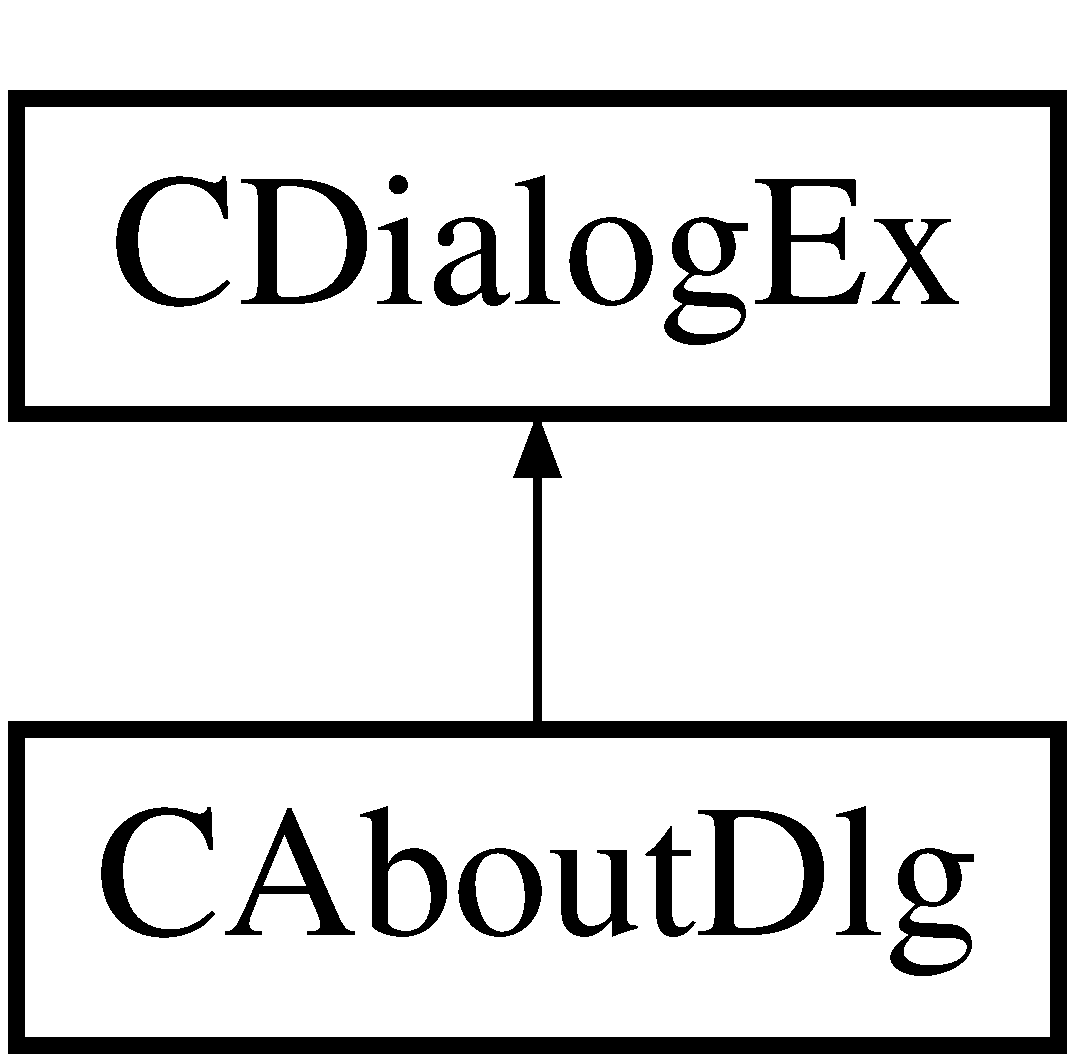
\includegraphics[height=2.000000cm]{class_c_about_dlg}
\end{center}
\end{figure}
\subsection*{Public Types}
\begin{DoxyCompactItemize}
\item 
\hypertarget{class_c_about_dlg_a27a5d4c47f16acb8562522fcd22871f7}{enum \{ {\bfseries I\+D\+D} = I\+D\+D\+\_\+\+A\+B\+O\+U\+T\+B\+O\+X
 \}}\label{class_c_about_dlg_a27a5d4c47f16acb8562522fcd22871f7}

\end{DoxyCompactItemize}
\subsection*{Public Member Functions}
\begin{DoxyCompactItemize}
\item 
\hyperlink{class_c_about_dlg_a6d1e6a33fef23bee6e75254189d865ce}{C\+About\+Dlg} ()
\end{DoxyCompactItemize}
\subsection*{Protected Member Functions}
\begin{DoxyCompactItemize}
\item 
virtual void \hyperlink{class_c_about_dlg_ab83db7484fec957282d7d5a21aed4df4}{Do\+Data\+Exchange} (C\+Data\+Exchange $\ast$p\+D\+X)
\end{DoxyCompactItemize}


\subsection{Detailed Description}
The About dialog box 

\subsection{Constructor \& Destructor Documentation}
\hypertarget{class_c_about_dlg_a6d1e6a33fef23bee6e75254189d865ce}{\index{C\+About\+Dlg@{C\+About\+Dlg}!C\+About\+Dlg@{C\+About\+Dlg}}
\index{C\+About\+Dlg@{C\+About\+Dlg}!C\+About\+Dlg@{C\+About\+Dlg}}
\subsubsection[{C\+About\+Dlg}]{\setlength{\rightskip}{0pt plus 5cm}C\+About\+Dlg\+::\+C\+About\+Dlg (
\begin{DoxyParamCaption}
{}
\end{DoxyParamCaption}
)}}\label{class_c_about_dlg_a6d1e6a33fef23bee6e75254189d865ce}
Constructor 

\subsection{Member Function Documentation}
\hypertarget{class_c_about_dlg_ab83db7484fec957282d7d5a21aed4df4}{\index{C\+About\+Dlg@{C\+About\+Dlg}!Do\+Data\+Exchange@{Do\+Data\+Exchange}}
\index{Do\+Data\+Exchange@{Do\+Data\+Exchange}!C\+About\+Dlg@{C\+About\+Dlg}}
\subsubsection[{Do\+Data\+Exchange}]{\setlength{\rightskip}{0pt plus 5cm}void C\+About\+Dlg\+::\+Do\+Data\+Exchange (
\begin{DoxyParamCaption}
\item[{C\+Data\+Exchange $\ast$}]{p\+D\+X}
\end{DoxyParamCaption}
)\hspace{0.3cm}{\ttfamily [protected]}, {\ttfamily [virtual]}}}\label{class_c_about_dlg_ab83db7484fec957282d7d5a21aed4df4}
Exchange data between the class and the dialog box 
\begin{DoxyParams}{Parameters}
{\em p\+D\+X} & structure that controls the data exchange \\
\hline
\end{DoxyParams}


The documentation for this class was generated from the following file\+:\begin{DoxyCompactItemize}
\item 
\hyperlink{_canadian_experience_8cpp}{Canadian\+Experience.\+cpp}\end{DoxyCompactItemize}

\hypertarget{class_c_actor}{\section{C\+Actor Class Reference}
\label{class_c_actor}\index{C\+Actor@{C\+Actor}}
}


{\ttfamily \#include $<$Actor.\+h$>$}

\subsection*{Public Member Functions}
\begin{DoxyCompactItemize}
\item 
\hyperlink{class_c_actor_a2849f9370b66ddeaa727c8b7045d62c2}{C\+Actor} (const std\+::wstring \&name)
\item 
\hyperlink{class_c_actor_ae7683d5f0b3edc85dc47850fa71de40f}{C\+Actor} ()=delete
\item 
\hyperlink{class_c_actor_a8af986ad4ec530967f942aaebd853632}{C\+Actor} (const \hyperlink{class_c_actor}{C\+Actor} \&)=delete
\item 
void \hyperlink{class_c_actor_aa947810cfb2f45129b501296bcad837c}{operator=} (const \hyperlink{class_c_actor}{C\+Actor} \&)=delete
\item 
virtual \hyperlink{class_c_actor_adca86a138fd9af275352336848ebad27}{$\sim$\+C\+Actor} ()
\item 
void \hyperlink{class_c_actor_af0417205281ecd3bc52a367724cc6635}{Set\+Root} (std\+::shared\+\_\+ptr$<$ \hyperlink{class_c_drawable}{C\+Drawable} $>$ root)
\item 
void \hyperlink{class_c_actor_a78048c684b231e498184d963b57fffe2}{Draw} (Gdiplus\+::\+Graphics $\ast$graphics)
\item 
std\+::shared\+\_\+ptr$<$ \hyperlink{class_c_drawable}{C\+Drawable} $>$ \hyperlink{class_c_actor_a63676c04fa760cd9fc56d85cb0542cd1}{Hit\+Test} (Gdiplus\+::\+Point pos)
\item 
void \hyperlink{class_c_actor_a943e05a65bde59998079ab647ec0e7ec}{Add\+Drawable} (std\+::shared\+\_\+ptr$<$ \hyperlink{class_c_drawable}{C\+Drawable} $>$ drawable)
\item 
std\+::wstring \hyperlink{class_c_actor_aee85c15c97f5f9652cb4c083772798e6}{Get\+Name} () const 
\item 
Gdiplus\+::\+Point \hyperlink{class_c_actor_ae3c531320a80c83419b4239c3227192b}{Get\+Position} () const 
\item 
void \hyperlink{class_c_actor_a4af7bf0c9c0bf4a41a99ad270ac4f1ca}{Set\+Picture} (\hyperlink{class_c_picture}{C\+Picture} $\ast$pic)
\item 
\hyperlink{class_c_picture}{C\+Picture} $\ast$ \hyperlink{class_c_actor_af94c21dd8535aaa4992904cdbec27b84}{Get\+Picture} ()
\item 
void \hyperlink{class_c_actor_af0bda8fd0ba0320f9fd6e67b7b16a07d}{Set\+Position} (Gdiplus\+::\+Point pos)
\item 
bool \hyperlink{class_c_actor_ab3e78932aeb9e2a764670bc82ac85094}{Is\+Enabled} () const 
\item 
void \hyperlink{class_c_actor_a6f9009e9753b07a00266cac01af2fdad}{Set\+Enabled} (bool enabled)
\item 
bool \hyperlink{class_c_actor_a2a5738cceea3dc667611ba4c4d9a5db4}{Is\+Clickable} () const 
\item 
void \hyperlink{class_c_actor_a6c717ba1037b3055a5ec94e18e1707de}{Set\+Clickable} (bool clickable)
\end{DoxyCompactItemize}


\subsection{Detailed Description}
Class for actors in our drawings.

An actor is some graphical object that consists of one or more parts. Actors can be animated. 

\subsection{Constructor \& Destructor Documentation}
\hypertarget{class_c_actor_a2849f9370b66ddeaa727c8b7045d62c2}{\index{C\+Actor@{C\+Actor}!C\+Actor@{C\+Actor}}
\index{C\+Actor@{C\+Actor}!C\+Actor@{C\+Actor}}
\subsubsection[{C\+Actor}]{\setlength{\rightskip}{0pt plus 5cm}C\+Actor\+::\+C\+Actor (
\begin{DoxyParamCaption}
\item[{const std\+::wstring \&}]{name}
\end{DoxyParamCaption}
)}}\label{class_c_actor_a2849f9370b66ddeaa727c8b7045d62c2}
Constructor 
\begin{DoxyParams}{Parameters}
{\em name} & The actor name \\
\hline
\end{DoxyParams}
\hypertarget{class_c_actor_ae7683d5f0b3edc85dc47850fa71de40f}{\index{C\+Actor@{C\+Actor}!C\+Actor@{C\+Actor}}
\index{C\+Actor@{C\+Actor}!C\+Actor@{C\+Actor}}
\subsubsection[{C\+Actor}]{\setlength{\rightskip}{0pt plus 5cm}C\+Actor\+::\+C\+Actor (
\begin{DoxyParamCaption}
{}
\end{DoxyParamCaption}
)\hspace{0.3cm}{\ttfamily [delete]}}}\label{class_c_actor_ae7683d5f0b3edc85dc47850fa71de40f}
Default constructor disabled \hypertarget{class_c_actor_a8af986ad4ec530967f942aaebd853632}{\index{C\+Actor@{C\+Actor}!C\+Actor@{C\+Actor}}
\index{C\+Actor@{C\+Actor}!C\+Actor@{C\+Actor}}
\subsubsection[{C\+Actor}]{\setlength{\rightskip}{0pt plus 5cm}C\+Actor\+::\+C\+Actor (
\begin{DoxyParamCaption}
\item[{const {\bf C\+Actor} \&}]{}
\end{DoxyParamCaption}
)\hspace{0.3cm}{\ttfamily [delete]}}}\label{class_c_actor_a8af986ad4ec530967f942aaebd853632}
Copy constructor disabled \hypertarget{class_c_actor_adca86a138fd9af275352336848ebad27}{\index{C\+Actor@{C\+Actor}!````~C\+Actor@{$\sim$\+C\+Actor}}
\index{````~C\+Actor@{$\sim$\+C\+Actor}!C\+Actor@{C\+Actor}}
\subsubsection[{$\sim$\+C\+Actor}]{\setlength{\rightskip}{0pt plus 5cm}C\+Actor\+::$\sim$\+C\+Actor (
\begin{DoxyParamCaption}
{}
\end{DoxyParamCaption}
)\hspace{0.3cm}{\ttfamily [virtual]}}}\label{class_c_actor_adca86a138fd9af275352336848ebad27}
Destructor 

\subsection{Member Function Documentation}
\hypertarget{class_c_actor_a943e05a65bde59998079ab647ec0e7ec}{\index{C\+Actor@{C\+Actor}!Add\+Drawable@{Add\+Drawable}}
\index{Add\+Drawable@{Add\+Drawable}!C\+Actor@{C\+Actor}}
\subsubsection[{Add\+Drawable}]{\setlength{\rightskip}{0pt plus 5cm}void C\+Actor\+::\+Add\+Drawable (
\begin{DoxyParamCaption}
\item[{std\+::shared\+\_\+ptr$<$ {\bf C\+Drawable} $>$}]{drawable}
\end{DoxyParamCaption}
)}}\label{class_c_actor_a943e05a65bde59998079ab647ec0e7ec}
add drawable


\begin{DoxyParams}{Parameters}
{\em drawable} & to draw\\
\hline
\end{DoxyParams}
Add a drawable to this actor 
\begin{DoxyParams}{Parameters}
{\em drawable} & The drawable to add \\
\hline
\end{DoxyParams}
\hypertarget{class_c_actor_a78048c684b231e498184d963b57fffe2}{\index{C\+Actor@{C\+Actor}!Draw@{Draw}}
\index{Draw@{Draw}!C\+Actor@{C\+Actor}}
\subsubsection[{Draw}]{\setlength{\rightskip}{0pt plus 5cm}void C\+Actor\+::\+Draw (
\begin{DoxyParamCaption}
\item[{Gdiplus\+::\+Graphics $\ast$}]{graphics}
\end{DoxyParamCaption}
)}}\label{class_c_actor_a78048c684b231e498184d963b57fffe2}
Draw


\begin{DoxyParams}{Parameters}
{\em graphics} & to draw on\\
\hline
\end{DoxyParams}
Draw this actor 
\begin{DoxyParams}{Parameters}
{\em graphics} & The Graphics object we are drawing on \\
\hline
\end{DoxyParams}
\hypertarget{class_c_actor_aee85c15c97f5f9652cb4c083772798e6}{\index{C\+Actor@{C\+Actor}!Get\+Name@{Get\+Name}}
\index{Get\+Name@{Get\+Name}!C\+Actor@{C\+Actor}}
\subsubsection[{Get\+Name}]{\setlength{\rightskip}{0pt plus 5cm}std\+::wstring C\+Actor\+::\+Get\+Name (
\begin{DoxyParamCaption}
{}
\end{DoxyParamCaption}
) const\hspace{0.3cm}{\ttfamily [inline]}}}\label{class_c_actor_aee85c15c97f5f9652cb4c083772798e6}
Get the actor name \begin{DoxyReturn}{Returns}
Actor name 
\end{DoxyReturn}
\hypertarget{class_c_actor_af94c21dd8535aaa4992904cdbec27b84}{\index{C\+Actor@{C\+Actor}!Get\+Picture@{Get\+Picture}}
\index{Get\+Picture@{Get\+Picture}!C\+Actor@{C\+Actor}}
\subsubsection[{Get\+Picture}]{\setlength{\rightskip}{0pt plus 5cm}{\bf C\+Picture}$\ast$ C\+Actor\+::\+Get\+Picture (
\begin{DoxyParamCaption}
{}
\end{DoxyParamCaption}
)\hspace{0.3cm}{\ttfamily [inline]}}}\label{class_c_actor_af94c21dd8535aaa4992904cdbec27b84}
Gets picture \begin{DoxyReturn}{Returns}
picture 
\end{DoxyReturn}
\hypertarget{class_c_actor_ae3c531320a80c83419b4239c3227192b}{\index{C\+Actor@{C\+Actor}!Get\+Position@{Get\+Position}}
\index{Get\+Position@{Get\+Position}!C\+Actor@{C\+Actor}}
\subsubsection[{Get\+Position}]{\setlength{\rightskip}{0pt plus 5cm}Gdiplus\+::\+Point C\+Actor\+::\+Get\+Position (
\begin{DoxyParamCaption}
{}
\end{DoxyParamCaption}
) const\hspace{0.3cm}{\ttfamily [inline]}}}\label{class_c_actor_ae3c531320a80c83419b4239c3227192b}
The actor position \begin{DoxyReturn}{Returns}
The actor position as a point 
\end{DoxyReturn}
\hypertarget{class_c_actor_a63676c04fa760cd9fc56d85cb0542cd1}{\index{C\+Actor@{C\+Actor}!Hit\+Test@{Hit\+Test}}
\index{Hit\+Test@{Hit\+Test}!C\+Actor@{C\+Actor}}
\subsubsection[{Hit\+Test}]{\setlength{\rightskip}{0pt plus 5cm}std\+::shared\+\_\+ptr$<$ {\bf C\+Drawable} $>$ C\+Actor\+::\+Hit\+Test (
\begin{DoxyParamCaption}
\item[{Gdiplus\+::\+Point}]{pos}
\end{DoxyParamCaption}
)}}\label{class_c_actor_a63676c04fa760cd9fc56d85cb0542cd1}
Hittest \begin{DoxyReturn}{Returns}
drawable object 
\end{DoxyReturn}

\begin{DoxyParams}{Parameters}
{\em pos} & position\\
\hline
\end{DoxyParams}
Test to see if a mouse click is on this actor. 
\begin{DoxyParams}{Parameters}
{\em pos} & Mouse position on drawing \\
\hline
\end{DoxyParams}
\begin{DoxyReturn}{Returns}
A drawable object we clicked on or nullptr if we missed. 
\end{DoxyReturn}
\hypertarget{class_c_actor_a2a5738cceea3dc667611ba4c4d9a5db4}{\index{C\+Actor@{C\+Actor}!Is\+Clickable@{Is\+Clickable}}
\index{Is\+Clickable@{Is\+Clickable}!C\+Actor@{C\+Actor}}
\subsubsection[{Is\+Clickable}]{\setlength{\rightskip}{0pt plus 5cm}bool C\+Actor\+::\+Is\+Clickable (
\begin{DoxyParamCaption}
{}
\end{DoxyParamCaption}
) const\hspace{0.3cm}{\ttfamily [inline]}}}\label{class_c_actor_a2a5738cceea3dc667611ba4c4d9a5db4}
Actor is clickable \begin{DoxyReturn}{Returns}
true if actor is clickable 
\end{DoxyReturn}
\hypertarget{class_c_actor_ab3e78932aeb9e2a764670bc82ac85094}{\index{C\+Actor@{C\+Actor}!Is\+Enabled@{Is\+Enabled}}
\index{Is\+Enabled@{Is\+Enabled}!C\+Actor@{C\+Actor}}
\subsubsection[{Is\+Enabled}]{\setlength{\rightskip}{0pt plus 5cm}bool C\+Actor\+::\+Is\+Enabled (
\begin{DoxyParamCaption}
{}
\end{DoxyParamCaption}
) const\hspace{0.3cm}{\ttfamily [inline]}}}\label{class_c_actor_ab3e78932aeb9e2a764670bc82ac85094}
Actor is enabled \begin{DoxyReturn}{Returns}
enabled status 
\end{DoxyReturn}
\hypertarget{class_c_actor_aa947810cfb2f45129b501296bcad837c}{\index{C\+Actor@{C\+Actor}!operator=@{operator=}}
\index{operator=@{operator=}!C\+Actor@{C\+Actor}}
\subsubsection[{operator=}]{\setlength{\rightskip}{0pt plus 5cm}void C\+Actor\+::operator= (
\begin{DoxyParamCaption}
\item[{const {\bf C\+Actor} \&}]{}
\end{DoxyParamCaption}
)\hspace{0.3cm}{\ttfamily [delete]}}}\label{class_c_actor_aa947810cfb2f45129b501296bcad837c}
Assignment operator disabled \hypertarget{class_c_actor_a6c717ba1037b3055a5ec94e18e1707de}{\index{C\+Actor@{C\+Actor}!Set\+Clickable@{Set\+Clickable}}
\index{Set\+Clickable@{Set\+Clickable}!C\+Actor@{C\+Actor}}
\subsubsection[{Set\+Clickable}]{\setlength{\rightskip}{0pt plus 5cm}void C\+Actor\+::\+Set\+Clickable (
\begin{DoxyParamCaption}
\item[{bool}]{clickable}
\end{DoxyParamCaption}
)\hspace{0.3cm}{\ttfamily [inline]}}}\label{class_c_actor_a6c717ba1037b3055a5ec94e18e1707de}
Actor clickable 
\begin{DoxyParams}{Parameters}
{\em clickable} & New clickable status \\
\hline
\end{DoxyParams}
\hypertarget{class_c_actor_a6f9009e9753b07a00266cac01af2fdad}{\index{C\+Actor@{C\+Actor}!Set\+Enabled@{Set\+Enabled}}
\index{Set\+Enabled@{Set\+Enabled}!C\+Actor@{C\+Actor}}
\subsubsection[{Set\+Enabled}]{\setlength{\rightskip}{0pt plus 5cm}void C\+Actor\+::\+Set\+Enabled (
\begin{DoxyParamCaption}
\item[{bool}]{enabled}
\end{DoxyParamCaption}
)\hspace{0.3cm}{\ttfamily [inline]}}}\label{class_c_actor_a6f9009e9753b07a00266cac01af2fdad}
Set Actor Enabled 
\begin{DoxyParams}{Parameters}
{\em enabled} & New enabled status \\
\hline
\end{DoxyParams}
\hypertarget{class_c_actor_a4af7bf0c9c0bf4a41a99ad270ac4f1ca}{\index{C\+Actor@{C\+Actor}!Set\+Picture@{Set\+Picture}}
\index{Set\+Picture@{Set\+Picture}!C\+Actor@{C\+Actor}}
\subsubsection[{Set\+Picture}]{\setlength{\rightskip}{0pt plus 5cm}void C\+Actor\+::\+Set\+Picture (
\begin{DoxyParamCaption}
\item[{{\bf C\+Picture} $\ast$}]{pic}
\end{DoxyParamCaption}
)\hspace{0.3cm}{\ttfamily [inline]}}}\label{class_c_actor_a4af7bf0c9c0bf4a41a99ad270ac4f1ca}
set pic


\begin{DoxyParams}{Parameters}
{\em pic} & to picrue \\
\hline
\end{DoxyParams}
\hypertarget{class_c_actor_af0bda8fd0ba0320f9fd6e67b7b16a07d}{\index{C\+Actor@{C\+Actor}!Set\+Position@{Set\+Position}}
\index{Set\+Position@{Set\+Position}!C\+Actor@{C\+Actor}}
\subsubsection[{Set\+Position}]{\setlength{\rightskip}{0pt plus 5cm}void C\+Actor\+::\+Set\+Position (
\begin{DoxyParamCaption}
\item[{Gdiplus\+::\+Point}]{pos}
\end{DoxyParamCaption}
)\hspace{0.3cm}{\ttfamily [inline]}}}\label{class_c_actor_af0bda8fd0ba0320f9fd6e67b7b16a07d}
The actor position 
\begin{DoxyParams}{Parameters}
{\em pos} & The new actor position \\
\hline
\end{DoxyParams}
\hypertarget{class_c_actor_af0417205281ecd3bc52a367724cc6635}{\index{C\+Actor@{C\+Actor}!Set\+Root@{Set\+Root}}
\index{Set\+Root@{Set\+Root}!C\+Actor@{C\+Actor}}
\subsubsection[{Set\+Root}]{\setlength{\rightskip}{0pt plus 5cm}void C\+Actor\+::\+Set\+Root (
\begin{DoxyParamCaption}
\item[{std\+::shared\+\_\+ptr$<$ {\bf C\+Drawable} $>$}]{root}
\end{DoxyParamCaption}
)}}\label{class_c_actor_af0417205281ecd3bc52a367724cc6635}
set root


\begin{DoxyParams}{Parameters}
{\em root} & to set\\
\hline
\end{DoxyParams}
Set the root drawable for the actor 
\begin{DoxyParams}{Parameters}
{\em root} & Pointer to root drawable \\
\hline
\end{DoxyParams}


The documentation for this class was generated from the following files\+:\begin{DoxyCompactItemize}
\item 
\hyperlink{_actor_8h}{Actor.\+h}\item 
\hyperlink{_actor_8cpp}{Actor.\+cpp}\end{DoxyCompactItemize}

\hypertarget{class_c_actor_factory}{\section{C\+Actor\+Factory Class Reference}
\label{class_c_actor_factory}\index{C\+Actor\+Factory@{C\+Actor\+Factory}}
}


{\ttfamily \#include $<$Actor\+Factory.\+h$>$}

Inheritance diagram for C\+Actor\+Factory\+:\begin{figure}[H]
\begin{center}
\leavevmode
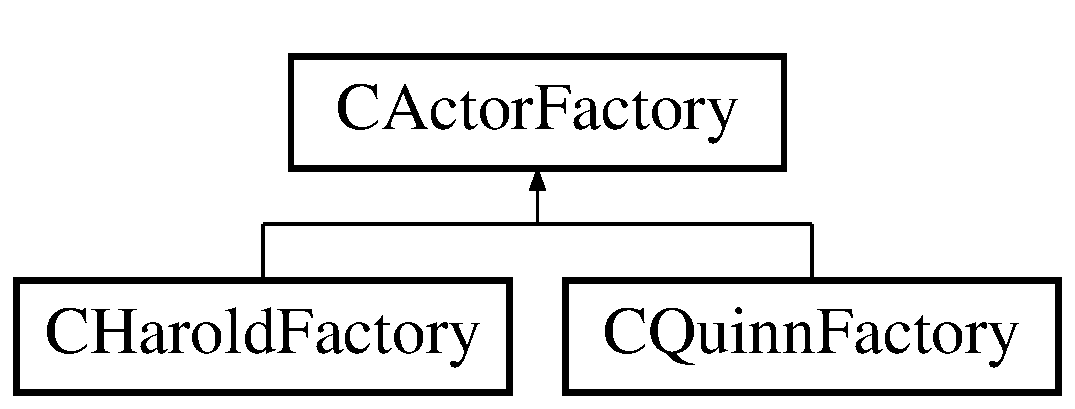
\includegraphics[height=2.000000cm]{class_c_actor_factory}
\end{center}
\end{figure}


\subsection{Detailed Description}
Abstract base class for actor factories. 

The documentation for this class was generated from the following files\+:\begin{DoxyCompactItemize}
\item 
\hyperlink{_actor_factory_8h}{Actor\+Factory.\+h}\item 
Actor\+Factory.\+cpp\end{DoxyCompactItemize}

\hypertarget{class_c_canadian_experience_app}{\section{C\+Canadian\+Experience\+App Class Reference}
\label{class_c_canadian_experience_app}\index{C\+Canadian\+Experience\+App@{C\+Canadian\+Experience\+App}}
}


{\ttfamily \#include $<$Canadian\+Experience.\+h$>$}

Inheritance diagram for C\+Canadian\+Experience\+App\+:\begin{figure}[H]
\begin{center}
\leavevmode
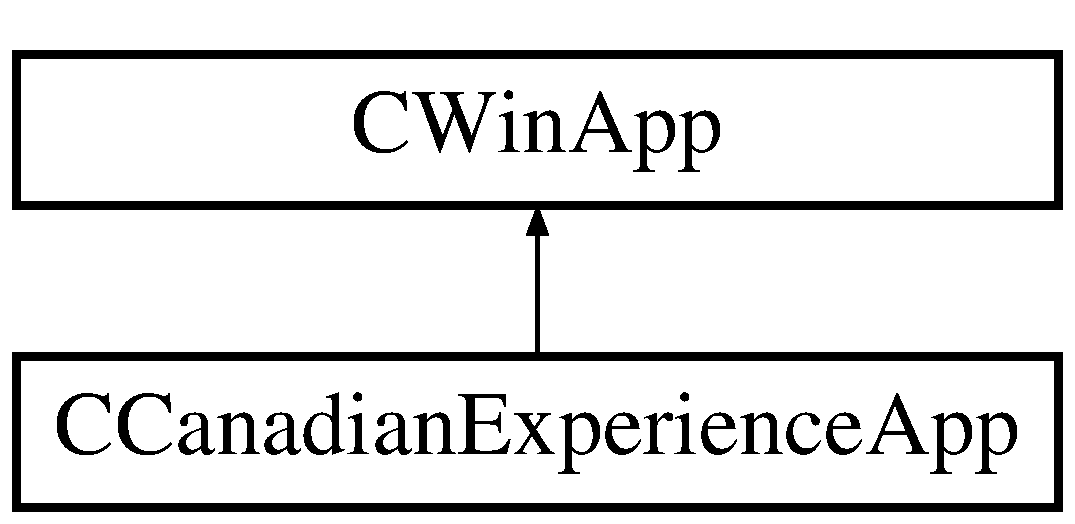
\includegraphics[height=2.000000cm]{class_c_canadian_experience_app}
\end{center}
\end{figure}
\subsection*{Public Member Functions}
\begin{DoxyCompactItemize}
\item 
\hyperlink{class_c_canadian_experience_app_a8a2d61bf478a5b12004e4f0d3c0c442a}{C\+Canadian\+Experience\+App} ()
\item 
virtual B\+O\+O\+L \hyperlink{class_c_canadian_experience_app_ab821deed5758f650a2fbbc65cefc8cc7}{Init\+Instance} ()
\item 
virtual int \hyperlink{class_c_canadian_experience_app_a289a9574888e0c922c455e73edf424ad}{Exit\+Instance} ()
\item 
afx\+\_\+msg void \hyperlink{class_c_canadian_experience_app_a99cb24a35f65d5821f7e09eefb0c97e7}{On\+App\+About} ()
\end{DoxyCompactItemize}


\subsection{Detailed Description}
Program application class 

\subsection{Constructor \& Destructor Documentation}
\hypertarget{class_c_canadian_experience_app_a8a2d61bf478a5b12004e4f0d3c0c442a}{\index{C\+Canadian\+Experience\+App@{C\+Canadian\+Experience\+App}!C\+Canadian\+Experience\+App@{C\+Canadian\+Experience\+App}}
\index{C\+Canadian\+Experience\+App@{C\+Canadian\+Experience\+App}!C\+Canadian\+Experience\+App@{C\+Canadian\+Experience\+App}}
\subsubsection[{C\+Canadian\+Experience\+App}]{\setlength{\rightskip}{0pt plus 5cm}C\+Canadian\+Experience\+App\+::\+C\+Canadian\+Experience\+App (
\begin{DoxyParamCaption}
{}
\end{DoxyParamCaption}
)}}\label{class_c_canadian_experience_app_a8a2d61bf478a5b12004e4f0d3c0c442a}
Constructor 

\subsection{Member Function Documentation}
\hypertarget{class_c_canadian_experience_app_a289a9574888e0c922c455e73edf424ad}{\index{C\+Canadian\+Experience\+App@{C\+Canadian\+Experience\+App}!Exit\+Instance@{Exit\+Instance}}
\index{Exit\+Instance@{Exit\+Instance}!C\+Canadian\+Experience\+App@{C\+Canadian\+Experience\+App}}
\subsubsection[{Exit\+Instance}]{\setlength{\rightskip}{0pt plus 5cm}int C\+Canadian\+Experience\+App\+::\+Exit\+Instance (
\begin{DoxyParamCaption}
{}
\end{DoxyParamCaption}
)\hspace{0.3cm}{\ttfamily [virtual]}}}\label{class_c_canadian_experience_app_a289a9574888e0c922c455e73edf424ad}
Exit this program \begin{DoxyReturn}{Returns}
exit code 
\end{DoxyReturn}
\hypertarget{class_c_canadian_experience_app_ab821deed5758f650a2fbbc65cefc8cc7}{\index{C\+Canadian\+Experience\+App@{C\+Canadian\+Experience\+App}!Init\+Instance@{Init\+Instance}}
\index{Init\+Instance@{Init\+Instance}!C\+Canadian\+Experience\+App@{C\+Canadian\+Experience\+App}}
\subsubsection[{Init\+Instance}]{\setlength{\rightskip}{0pt plus 5cm}B\+O\+O\+L C\+Canadian\+Experience\+App\+::\+Init\+Instance (
\begin{DoxyParamCaption}
{}
\end{DoxyParamCaption}
)\hspace{0.3cm}{\ttfamily [virtual]}}}\label{class_c_canadian_experience_app_ab821deed5758f650a2fbbc65cefc8cc7}
\hyperlink{class_c_canadian_experience_app}{C\+Canadian\+Experience\+App} initialization \begin{DoxyReturn}{Returns}
T\+R\+U\+E if successful 
\end{DoxyReturn}
\hypertarget{class_c_canadian_experience_app_a99cb24a35f65d5821f7e09eefb0c97e7}{\index{C\+Canadian\+Experience\+App@{C\+Canadian\+Experience\+App}!On\+App\+About@{On\+App\+About}}
\index{On\+App\+About@{On\+App\+About}!C\+Canadian\+Experience\+App@{C\+Canadian\+Experience\+App}}
\subsubsection[{On\+App\+About}]{\setlength{\rightskip}{0pt plus 5cm}void C\+Canadian\+Experience\+App\+::\+On\+App\+About (
\begin{DoxyParamCaption}
{}
\end{DoxyParamCaption}
)}}\label{class_c_canadian_experience_app_a99cb24a35f65d5821f7e09eefb0c97e7}
App command to run the dialog 

The documentation for this class was generated from the following files\+:\begin{DoxyCompactItemize}
\item 
\hyperlink{_canadian_experience_8h}{Canadian\+Experience.\+h}\item 
\hyperlink{_canadian_experience_8cpp}{Canadian\+Experience.\+cpp}\end{DoxyCompactItemize}

\hypertarget{class_c_drawable}{\section{C\+Drawable Class Reference}
\label{class_c_drawable}\index{C\+Drawable@{C\+Drawable}}
}


{\ttfamily \#include $<$Drawable.\+h$>$}

Inheritance diagram for C\+Drawable\+:\begin{figure}[H]
\begin{center}
\leavevmode
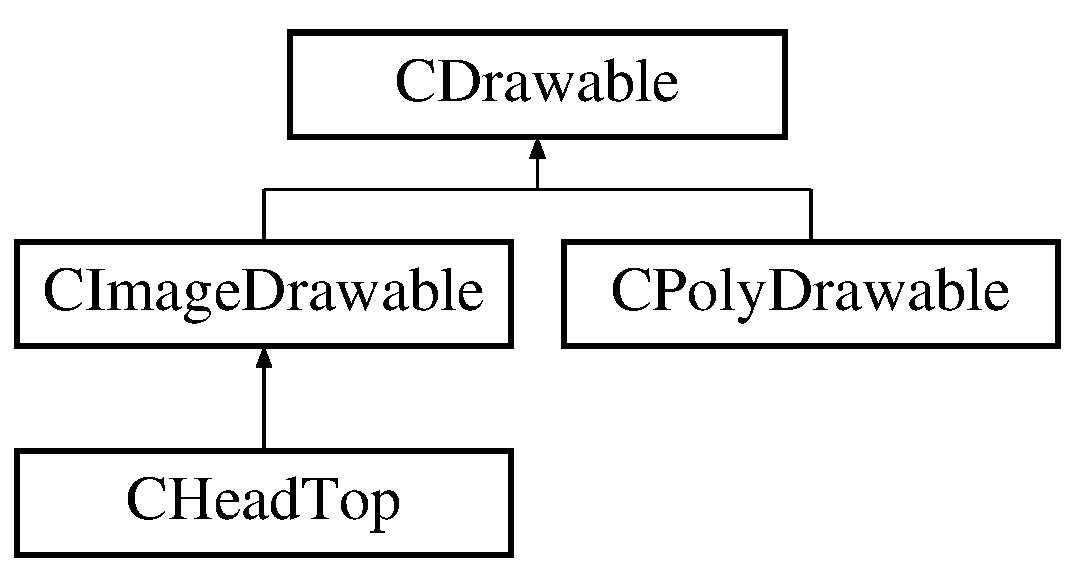
\includegraphics[height=3.000000cm]{class_c_drawable}
\end{center}
\end{figure}
\subsection*{Public Member Functions}
\begin{DoxyCompactItemize}
\item 
virtual \hyperlink{class_c_drawable_a58fd1036856d627b19976088e4143630}{$\sim$\+C\+Drawable} ()
\item 
\hyperlink{class_c_drawable_abd46d61baf3d5f5210aa3c66b98d9263}{C\+Drawable} ()=delete
\item 
\hyperlink{class_c_drawable_abec99c088c1a7c12e1d7ecae69135602}{C\+Drawable} (const \hyperlink{class_c_drawable}{C\+Drawable} \&)=delete
\item 
void \hyperlink{class_c_drawable_aabd5f52b903e57a4c8b145cb69158adb}{operator=} (const \hyperlink{class_c_drawable}{C\+Drawable} \&)=delete
\item 
void \hyperlink{class_c_drawable_a86762c6e220d9f502c6ccf9baf1135ac}{Set\+Actor} (\hyperlink{class_c_actor}{C\+Actor} $\ast$actor)
\item 
virtual void \hyperlink{class_c_drawable_a9b6a9920a75d88d9ae321997495eaec7}{Draw} (Gdiplus\+::\+Graphics $\ast$graphics)=0
\item 
void \hyperlink{class_c_drawable_ac154be14313b739471d3a1529a2b31b5}{Place} (Gdiplus\+::\+Point offset, double rotate)
\item 
void \hyperlink{class_c_drawable_ab636167462699dde9b80e6dcb08caf7c}{Add\+Child} (std\+::shared\+\_\+ptr$<$ \hyperlink{class_c_drawable}{C\+Drawable} $>$ child)
\item 
virtual bool \hyperlink{class_c_drawable_af715bc2e79788b2a44a74ad70b181544}{Hit\+Test} (Gdiplus\+::\+Point pos)=0
\item 
virtual bool \hyperlink{class_c_drawable_ac9f03cfc58aed75fb52cd69c71e7b6e0}{Is\+Movable} ()
\item 
void \hyperlink{class_c_drawable_a2241b02a5f50c7a455283a9fb24d5b27}{Move} (Gdiplus\+::\+Point delta)
\item 
void \hyperlink{class_c_drawable_aa6b8988df847a76c30dfcf525ab65449}{Set\+Position} (Gdiplus\+::\+Point pos)
\item 
Gdiplus\+::\+Point \hyperlink{class_c_drawable_ac1def1d34d8069e3985e3a423ba80f2d}{Get\+Position} () const 
\item 
void \hyperlink{class_c_drawable_ab1191ba99b869690839ff20cd0cc45c4}{Set\+Rotation} (double r)
\item 
double \hyperlink{class_c_drawable_afb31912cfe47cc336dfbef384181ca65}{Get\+Rotation} () const 
\item 
std\+::wstring \hyperlink{class_c_drawable_a45af045c285cd0be9340a9a0d9883260}{Get\+Name} () const 
\item 
void \hyperlink{class_c_drawable_ad53fc2430248f2ac022ab142024df983}{Set\+Parent} (\hyperlink{class_c_drawable}{C\+Drawable} $\ast$parent)
\item 
\hyperlink{class_c_drawable}{C\+Drawable} $\ast$ \hyperlink{class_c_drawable_ab09e86c9bb408d5e2756ab6b439a674c}{Get\+Parent} () const 
\end{DoxyCompactItemize}
\subsection*{Protected Member Functions}
\begin{DoxyCompactItemize}
\item 
\hyperlink{class_c_drawable_a2e153d7fd3a752139b0b87ea990a25fc}{C\+Drawable} (const std\+::wstring \&name)
\item 
Gdiplus\+::\+Point \hyperlink{class_c_drawable_aabf32ebc32a2dbe928bc9fa38bd82535}{Rotate\+Point} (Gdiplus\+::\+Point point, double angle)
\end{DoxyCompactItemize}
\subsection*{Protected Attributes}
\begin{DoxyCompactItemize}
\item 
\hypertarget{class_c_drawable_abafce2c99898aac71bdb99ec2031d3a5}{Gdiplus\+::\+Point \hyperlink{class_c_drawable_abafce2c99898aac71bdb99ec2031d3a5}{m\+Placed\+Position} = Gdiplus\+::\+Point(0, 0)}\label{class_c_drawable_abafce2c99898aac71bdb99ec2031d3a5}

\begin{DoxyCompactList}\small\item\em The actual postion in the drawing. \end{DoxyCompactList}\item 
\hypertarget{class_c_drawable_a3b280b16b1a4a8c6e2588b1dc5574bda}{double \hyperlink{class_c_drawable_a3b280b16b1a4a8c6e2588b1dc5574bda}{m\+Placed\+R} = 0}\label{class_c_drawable_a3b280b16b1a4a8c6e2588b1dc5574bda}

\begin{DoxyCompactList}\small\item\em The actual rotation in the drawing. \end{DoxyCompactList}\end{DoxyCompactItemize}


\subsection{Detailed Description}
Abstract base class for drawable elements of our picture 

\subsection{Constructor \& Destructor Documentation}
\hypertarget{class_c_drawable_a58fd1036856d627b19976088e4143630}{\index{C\+Drawable@{C\+Drawable}!````~C\+Drawable@{$\sim$\+C\+Drawable}}
\index{````~C\+Drawable@{$\sim$\+C\+Drawable}!C\+Drawable@{C\+Drawable}}
\subsubsection[{$\sim$\+C\+Drawable}]{\setlength{\rightskip}{0pt plus 5cm}C\+Drawable\+::$\sim$\+C\+Drawable (
\begin{DoxyParamCaption}
{}
\end{DoxyParamCaption}
)\hspace{0.3cm}{\ttfamily [virtual]}}}\label{class_c_drawable_a58fd1036856d627b19976088e4143630}
destructor

Destructor \hypertarget{class_c_drawable_abd46d61baf3d5f5210aa3c66b98d9263}{\index{C\+Drawable@{C\+Drawable}!C\+Drawable@{C\+Drawable}}
\index{C\+Drawable@{C\+Drawable}!C\+Drawable@{C\+Drawable}}
\subsubsection[{C\+Drawable}]{\setlength{\rightskip}{0pt plus 5cm}C\+Drawable\+::\+C\+Drawable (
\begin{DoxyParamCaption}
{}
\end{DoxyParamCaption}
)\hspace{0.3cm}{\ttfamily [delete]}}}\label{class_c_drawable_abd46d61baf3d5f5210aa3c66b98d9263}
Default constructor disabled \hypertarget{class_c_drawable_abec99c088c1a7c12e1d7ecae69135602}{\index{C\+Drawable@{C\+Drawable}!C\+Drawable@{C\+Drawable}}
\index{C\+Drawable@{C\+Drawable}!C\+Drawable@{C\+Drawable}}
\subsubsection[{C\+Drawable}]{\setlength{\rightskip}{0pt plus 5cm}C\+Drawable\+::\+C\+Drawable (
\begin{DoxyParamCaption}
\item[{const {\bf C\+Drawable} \&}]{}
\end{DoxyParamCaption}
)\hspace{0.3cm}{\ttfamily [delete]}}}\label{class_c_drawable_abec99c088c1a7c12e1d7ecae69135602}
Copy constructor disabled \hypertarget{class_c_drawable_a2e153d7fd3a752139b0b87ea990a25fc}{\index{C\+Drawable@{C\+Drawable}!C\+Drawable@{C\+Drawable}}
\index{C\+Drawable@{C\+Drawable}!C\+Drawable@{C\+Drawable}}
\subsubsection[{C\+Drawable}]{\setlength{\rightskip}{0pt plus 5cm}C\+Drawable\+::\+C\+Drawable (
\begin{DoxyParamCaption}
\item[{const std\+::wstring \&}]{name}
\end{DoxyParamCaption}
)\hspace{0.3cm}{\ttfamily [protected]}}}\label{class_c_drawable_a2e153d7fd3a752139b0b87ea990a25fc}
Constructor 
\begin{DoxyParams}{Parameters}
{\em name} & is name to draw\\
\hline
\end{DoxyParams}
Constructor 
\begin{DoxyParams}{Parameters}
{\em name} & The drawable name \\
\hline
\end{DoxyParams}


\subsection{Member Function Documentation}
\hypertarget{class_c_drawable_ab636167462699dde9b80e6dcb08caf7c}{\index{C\+Drawable@{C\+Drawable}!Add\+Child@{Add\+Child}}
\index{Add\+Child@{Add\+Child}!C\+Drawable@{C\+Drawable}}
\subsubsection[{Add\+Child}]{\setlength{\rightskip}{0pt plus 5cm}void C\+Drawable\+::\+Add\+Child (
\begin{DoxyParamCaption}
\item[{std\+::shared\+\_\+ptr$<$ {\bf C\+Drawable} $>$}]{child}
\end{DoxyParamCaption}
)}}\label{class_c_drawable_ab636167462699dde9b80e6dcb08caf7c}
Add child 
\begin{DoxyParams}{Parameters}
{\em child} & thing we are adding.\\
\hline
\end{DoxyParams}
Add a child drawable to this drawable 
\begin{DoxyParams}{Parameters}
{\em child} & The child to add \\
\hline
\end{DoxyParams}
\hypertarget{class_c_drawable_a9b6a9920a75d88d9ae321997495eaec7}{\index{C\+Drawable@{C\+Drawable}!Draw@{Draw}}
\index{Draw@{Draw}!C\+Drawable@{C\+Drawable}}
\subsubsection[{Draw}]{\setlength{\rightskip}{0pt plus 5cm}virtual void C\+Drawable\+::\+Draw (
\begin{DoxyParamCaption}
\item[{Gdiplus\+::\+Graphics $\ast$}]{graphics}
\end{DoxyParamCaption}
)\hspace{0.3cm}{\ttfamily [pure virtual]}}}\label{class_c_drawable_a9b6a9920a75d88d9ae321997495eaec7}
Draw 
\begin{DoxyParams}{Parameters}
{\em graphics} & graphics we are drawing \\
\hline
\end{DoxyParams}


Implemented in \hyperlink{class_c_image_drawable_abf591e6f5e92537119ab745eba054bd1}{C\+Image\+Drawable}, \hyperlink{class_c_poly_drawable_a30d59469ee2db1cd0bf786ffff031bdf}{C\+Poly\+Drawable}, and \hyperlink{class_c_head_top_aa77d9fa703079ee68a4e4e8e3c816932}{C\+Head\+Top}.

\hypertarget{class_c_drawable_a45af045c285cd0be9340a9a0d9883260}{\index{C\+Drawable@{C\+Drawable}!Get\+Name@{Get\+Name}}
\index{Get\+Name@{Get\+Name}!C\+Drawable@{C\+Drawable}}
\subsubsection[{Get\+Name}]{\setlength{\rightskip}{0pt plus 5cm}std\+::wstring C\+Drawable\+::\+Get\+Name (
\begin{DoxyParamCaption}
{}
\end{DoxyParamCaption}
) const\hspace{0.3cm}{\ttfamily [inline]}}}\label{class_c_drawable_a45af045c285cd0be9340a9a0d9883260}
Get the drawable name \begin{DoxyReturn}{Returns}
The drawable name 
\end{DoxyReturn}
\hypertarget{class_c_drawable_ab09e86c9bb408d5e2756ab6b439a674c}{\index{C\+Drawable@{C\+Drawable}!Get\+Parent@{Get\+Parent}}
\index{Get\+Parent@{Get\+Parent}!C\+Drawable@{C\+Drawable}}
\subsubsection[{Get\+Parent}]{\setlength{\rightskip}{0pt plus 5cm}{\bf C\+Drawable}$\ast$ C\+Drawable\+::\+Get\+Parent (
\begin{DoxyParamCaption}
{}
\end{DoxyParamCaption}
) const\hspace{0.3cm}{\ttfamily [inline]}}}\label{class_c_drawable_ab09e86c9bb408d5e2756ab6b439a674c}
Getter for a variable \begin{DoxyReturn}{Returns}
parent for getting 
\end{DoxyReturn}
\hypertarget{class_c_drawable_ac1def1d34d8069e3985e3a423ba80f2d}{\index{C\+Drawable@{C\+Drawable}!Get\+Position@{Get\+Position}}
\index{Get\+Position@{Get\+Position}!C\+Drawable@{C\+Drawable}}
\subsubsection[{Get\+Position}]{\setlength{\rightskip}{0pt plus 5cm}Gdiplus\+::\+Point C\+Drawable\+::\+Get\+Position (
\begin{DoxyParamCaption}
{}
\end{DoxyParamCaption}
) const\hspace{0.3cm}{\ttfamily [inline]}}}\label{class_c_drawable_ac1def1d34d8069e3985e3a423ba80f2d}
Get the drawable position \begin{DoxyReturn}{Returns}
The drawable position 
\end{DoxyReturn}
\hypertarget{class_c_drawable_afb31912cfe47cc336dfbef384181ca65}{\index{C\+Drawable@{C\+Drawable}!Get\+Rotation@{Get\+Rotation}}
\index{Get\+Rotation@{Get\+Rotation}!C\+Drawable@{C\+Drawable}}
\subsubsection[{Get\+Rotation}]{\setlength{\rightskip}{0pt plus 5cm}double C\+Drawable\+::\+Get\+Rotation (
\begin{DoxyParamCaption}
{}
\end{DoxyParamCaption}
) const\hspace{0.3cm}{\ttfamily [inline]}}}\label{class_c_drawable_afb31912cfe47cc336dfbef384181ca65}
Get the rotation angle in radians \begin{DoxyReturn}{Returns}
The rotation angle in radians 
\end{DoxyReturn}
\hypertarget{class_c_drawable_af715bc2e79788b2a44a74ad70b181544}{\index{C\+Drawable@{C\+Drawable}!Hit\+Test@{Hit\+Test}}
\index{Hit\+Test@{Hit\+Test}!C\+Drawable@{C\+Drawable}}
\subsubsection[{Hit\+Test}]{\setlength{\rightskip}{0pt plus 5cm}virtual bool C\+Drawable\+::\+Hit\+Test (
\begin{DoxyParamCaption}
\item[{Gdiplus\+::\+Point}]{pos}
\end{DoxyParamCaption}
)\hspace{0.3cm}{\ttfamily [pure virtual]}}}\label{class_c_drawable_af715bc2e79788b2a44a74ad70b181544}
Hit test 
\begin{DoxyParams}{Parameters}
{\em pos} & position \\
\hline
\end{DoxyParams}


Implemented in \hyperlink{class_c_image_drawable_ac9f173d9fcb21dbb45f4cbf4593a6984}{C\+Image\+Drawable}, and \hyperlink{class_c_poly_drawable_af45e78d42d9eee657e0bedde0fe003e4}{C\+Poly\+Drawable}.

\hypertarget{class_c_drawable_ac9f03cfc58aed75fb52cd69c71e7b6e0}{\index{C\+Drawable@{C\+Drawable}!Is\+Movable@{Is\+Movable}}
\index{Is\+Movable@{Is\+Movable}!C\+Drawable@{C\+Drawable}}
\subsubsection[{Is\+Movable}]{\setlength{\rightskip}{0pt plus 5cm}virtual bool C\+Drawable\+::\+Is\+Movable (
\begin{DoxyParamCaption}
{}
\end{DoxyParamCaption}
)\hspace{0.3cm}{\ttfamily [inline]}, {\ttfamily [virtual]}}}\label{class_c_drawable_ac9f03cfc58aed75fb52cd69c71e7b6e0}
Is\+Moveable \begin{DoxyReturn}{Returns}
false 
\end{DoxyReturn}


Reimplemented in \hyperlink{class_c_head_top_a38d98789668f640fa3bbb8352fb54c49}{C\+Head\+Top}.

\hypertarget{class_c_drawable_a2241b02a5f50c7a455283a9fb24d5b27}{\index{C\+Drawable@{C\+Drawable}!Move@{Move}}
\index{Move@{Move}!C\+Drawable@{C\+Drawable}}
\subsubsection[{Move}]{\setlength{\rightskip}{0pt plus 5cm}void C\+Drawable\+::\+Move (
\begin{DoxyParamCaption}
\item[{Gdiplus\+::\+Point}]{delta}
\end{DoxyParamCaption}
)}}\label{class_c_drawable_a2241b02a5f50c7a455283a9fb24d5b27}
Move 
\begin{DoxyParams}{Parameters}
{\em delta} & is a point\\
\hline
\end{DoxyParams}
Move this drawable some amount 
\begin{DoxyParams}{Parameters}
{\em delta} & The amount to move \\
\hline
\end{DoxyParams}
\hypertarget{class_c_drawable_aabd5f52b903e57a4c8b145cb69158adb}{\index{C\+Drawable@{C\+Drawable}!operator=@{operator=}}
\index{operator=@{operator=}!C\+Drawable@{C\+Drawable}}
\subsubsection[{operator=}]{\setlength{\rightskip}{0pt plus 5cm}void C\+Drawable\+::operator= (
\begin{DoxyParamCaption}
\item[{const {\bf C\+Drawable} \&}]{}
\end{DoxyParamCaption}
)\hspace{0.3cm}{\ttfamily [delete]}}}\label{class_c_drawable_aabd5f52b903e57a4c8b145cb69158adb}
Assignment operator disabled \hypertarget{class_c_drawable_ac154be14313b739471d3a1529a2b31b5}{\index{C\+Drawable@{C\+Drawable}!Place@{Place}}
\index{Place@{Place}!C\+Drawable@{C\+Drawable}}
\subsubsection[{Place}]{\setlength{\rightskip}{0pt plus 5cm}void C\+Drawable\+::\+Place (
\begin{DoxyParamCaption}
\item[{Gdiplus\+::\+Point}]{offset, }
\item[{double}]{rotate}
\end{DoxyParamCaption}
)}}\label{class_c_drawable_ac154be14313b739471d3a1529a2b31b5}
Place 
\begin{DoxyParams}{Parameters}
{\em offset} & amount offset is moved by \\
\hline
{\em rotate} & amount we are rotating.\\
\hline
\end{DoxyParams}
Place this drawable relative to its parent

This works hierarchically from top item down. 
\begin{DoxyParams}{Parameters}
{\em offset} & Parent offset \\
\hline
{\em rotate} & Parent rotation \\
\hline
\end{DoxyParams}
\hypertarget{class_c_drawable_aabf32ebc32a2dbe928bc9fa38bd82535}{\index{C\+Drawable@{C\+Drawable}!Rotate\+Point@{Rotate\+Point}}
\index{Rotate\+Point@{Rotate\+Point}!C\+Drawable@{C\+Drawable}}
\subsubsection[{Rotate\+Point}]{\setlength{\rightskip}{0pt plus 5cm}Gdiplus\+::\+Point C\+Drawable\+::\+Rotate\+Point (
\begin{DoxyParamCaption}
\item[{Gdiplus\+::\+Point}]{point, }
\item[{double}]{angle}
\end{DoxyParamCaption}
)\hspace{0.3cm}{\ttfamily [protected]}}}\label{class_c_drawable_aabf32ebc32a2dbe928bc9fa38bd82535}
Rotate Point 
\begin{DoxyParams}{Parameters}
{\em point} & is the point \\
\hline
{\em angle} & is angle of rotate\\
\hline
\end{DoxyParams}
Rotate a point by a given angle. 
\begin{DoxyParams}{Parameters}
{\em point} & The point to rotate \\
\hline
{\em angle} & An angle in radians \\
\hline
\end{DoxyParams}
\begin{DoxyReturn}{Returns}
Rotated point 
\end{DoxyReturn}
\hypertarget{class_c_drawable_a86762c6e220d9f502c6ccf9baf1135ac}{\index{C\+Drawable@{C\+Drawable}!Set\+Actor@{Set\+Actor}}
\index{Set\+Actor@{Set\+Actor}!C\+Drawable@{C\+Drawable}}
\subsubsection[{Set\+Actor}]{\setlength{\rightskip}{0pt plus 5cm}void C\+Drawable\+::\+Set\+Actor (
\begin{DoxyParamCaption}
\item[{{\bf C\+Actor} $\ast$}]{actor}
\end{DoxyParamCaption}
)}}\label{class_c_drawable_a86762c6e220d9f502c6ccf9baf1135ac}
Set Actor 
\begin{DoxyParams}{Parameters}
{\em actor} & actor that we are setting\\
\hline
\end{DoxyParams}
Set the actor using this drawable 
\begin{DoxyParams}{Parameters}
{\em actor} & Actor using this drawable \\
\hline
\end{DoxyParams}
\hypertarget{class_c_drawable_ad53fc2430248f2ac022ab142024df983}{\index{C\+Drawable@{C\+Drawable}!Set\+Parent@{Set\+Parent}}
\index{Set\+Parent@{Set\+Parent}!C\+Drawable@{C\+Drawable}}
\subsubsection[{Set\+Parent}]{\setlength{\rightskip}{0pt plus 5cm}void C\+Drawable\+::\+Set\+Parent (
\begin{DoxyParamCaption}
\item[{{\bf C\+Drawable} $\ast$}]{parent}
\end{DoxyParamCaption}
)\hspace{0.3cm}{\ttfamily [inline]}}}\label{class_c_drawable_ad53fc2430248f2ac022ab142024df983}
Setter for a variable 
\begin{DoxyParams}{Parameters}
{\em parent} & to change to \\
\hline
\end{DoxyParams}
\hypertarget{class_c_drawable_aa6b8988df847a76c30dfcf525ab65449}{\index{C\+Drawable@{C\+Drawable}!Set\+Position@{Set\+Position}}
\index{Set\+Position@{Set\+Position}!C\+Drawable@{C\+Drawable}}
\subsubsection[{Set\+Position}]{\setlength{\rightskip}{0pt plus 5cm}void C\+Drawable\+::\+Set\+Position (
\begin{DoxyParamCaption}
\item[{Gdiplus\+::\+Point}]{pos}
\end{DoxyParamCaption}
)\hspace{0.3cm}{\ttfamily [inline]}}}\label{class_c_drawable_aa6b8988df847a76c30dfcf525ab65449}
Set the drawable position 
\begin{DoxyParams}{Parameters}
{\em pos} & The new drawable position \\
\hline
\end{DoxyParams}
\hypertarget{class_c_drawable_ab1191ba99b869690839ff20cd0cc45c4}{\index{C\+Drawable@{C\+Drawable}!Set\+Rotation@{Set\+Rotation}}
\index{Set\+Rotation@{Set\+Rotation}!C\+Drawable@{C\+Drawable}}
\subsubsection[{Set\+Rotation}]{\setlength{\rightskip}{0pt plus 5cm}void C\+Drawable\+::\+Set\+Rotation (
\begin{DoxyParamCaption}
\item[{double}]{r}
\end{DoxyParamCaption}
)\hspace{0.3cm}{\ttfamily [inline]}}}\label{class_c_drawable_ab1191ba99b869690839ff20cd0cc45c4}
Set the rotation angle in radians 
\begin{DoxyParams}{Parameters}
{\em r} & The new rotation angle in radians \\
\hline
\end{DoxyParams}


The documentation for this class was generated from the following files\+:\begin{DoxyCompactItemize}
\item 
\hyperlink{_drawable_8h}{Drawable.\+h}\item 
\hyperlink{_drawable_8cpp}{Drawable.\+cpp}\end{DoxyCompactItemize}

\hypertarget{class_c_harold_factory}{\section{C\+Harold\+Factory Class Reference}
\label{class_c_harold_factory}\index{C\+Harold\+Factory@{C\+Harold\+Factory}}
}


{\ttfamily \#include $<$Harold\+Factory.\+h$>$}

Inheritance diagram for C\+Harold\+Factory\+:\begin{figure}[H]
\begin{center}
\leavevmode
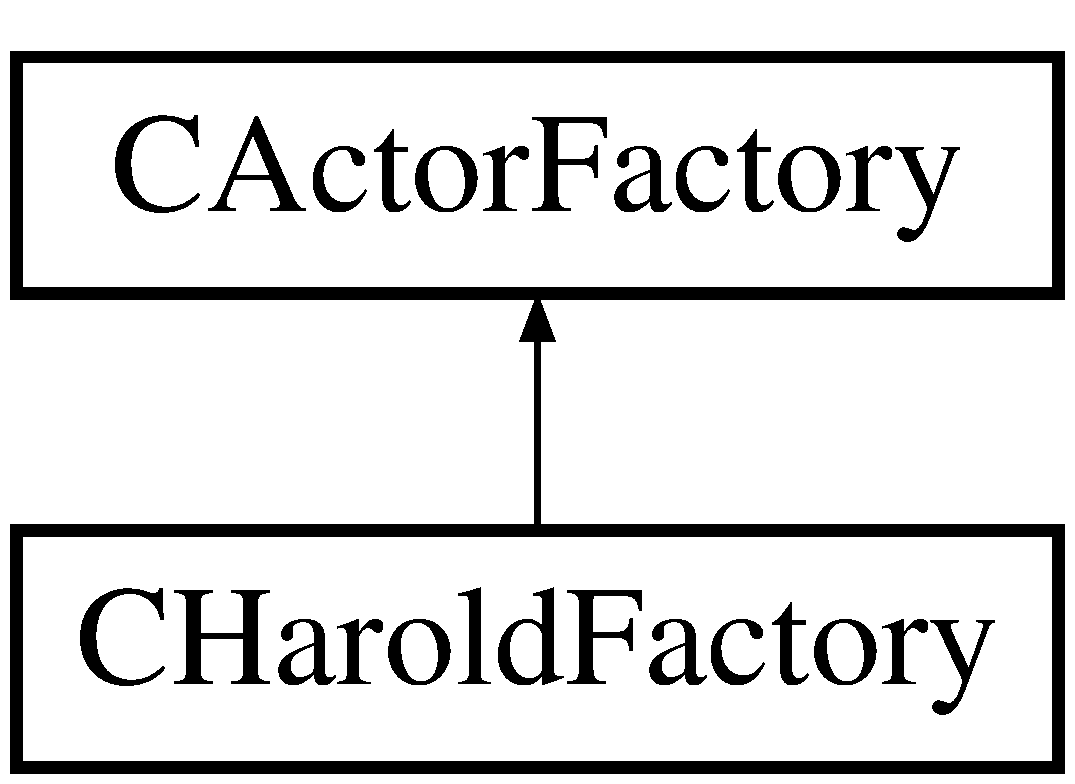
\includegraphics[height=2.000000cm]{class_c_harold_factory}
\end{center}
\end{figure}
\subsection*{Public Member Functions}
\begin{DoxyCompactItemize}
\item 
std\+::shared\+\_\+ptr$<$ \hyperlink{class_c_actor}{C\+Actor} $>$ \hyperlink{class_c_harold_factory_a785f8194f83d866bfc2a237fc3d4abc1}{Create} ()
\end{DoxyCompactItemize}


\subsection{Detailed Description}
Factory class that builds the Harold character 

\subsection{Member Function Documentation}
\hypertarget{class_c_harold_factory_a785f8194f83d866bfc2a237fc3d4abc1}{\index{C\+Harold\+Factory@{C\+Harold\+Factory}!Create@{Create}}
\index{Create@{Create}!C\+Harold\+Factory@{C\+Harold\+Factory}}
\subsubsection[{Create}]{\setlength{\rightskip}{0pt plus 5cm}std\+::shared\+\_\+ptr$<$ {\bf C\+Actor} $>$ C\+Harold\+Factory\+::\+Create (
\begin{DoxyParamCaption}
{}
\end{DoxyParamCaption}
)}}\label{class_c_harold_factory_a785f8194f83d866bfc2a237fc3d4abc1}
This is a concrete factory method that creates our Harold actor. \begin{DoxyReturn}{Returns}
Pointer to an actor object. 
\end{DoxyReturn}


The documentation for this class was generated from the following files\+:\begin{DoxyCompactItemize}
\item 
\hyperlink{_harold_factory_8h}{Harold\+Factory.\+h}\item 
Harold\+Factory.\+cpp\end{DoxyCompactItemize}

\hypertarget{class_c_head_top}{\section{C\+Head\+Top Class Reference}
\label{class_c_head_top}\index{C\+Head\+Top@{C\+Head\+Top}}
}


{\ttfamily \#include $<$Head\+Top.\+h$>$}

Inheritance diagram for C\+Head\+Top\+:\begin{figure}[H]
\begin{center}
\leavevmode
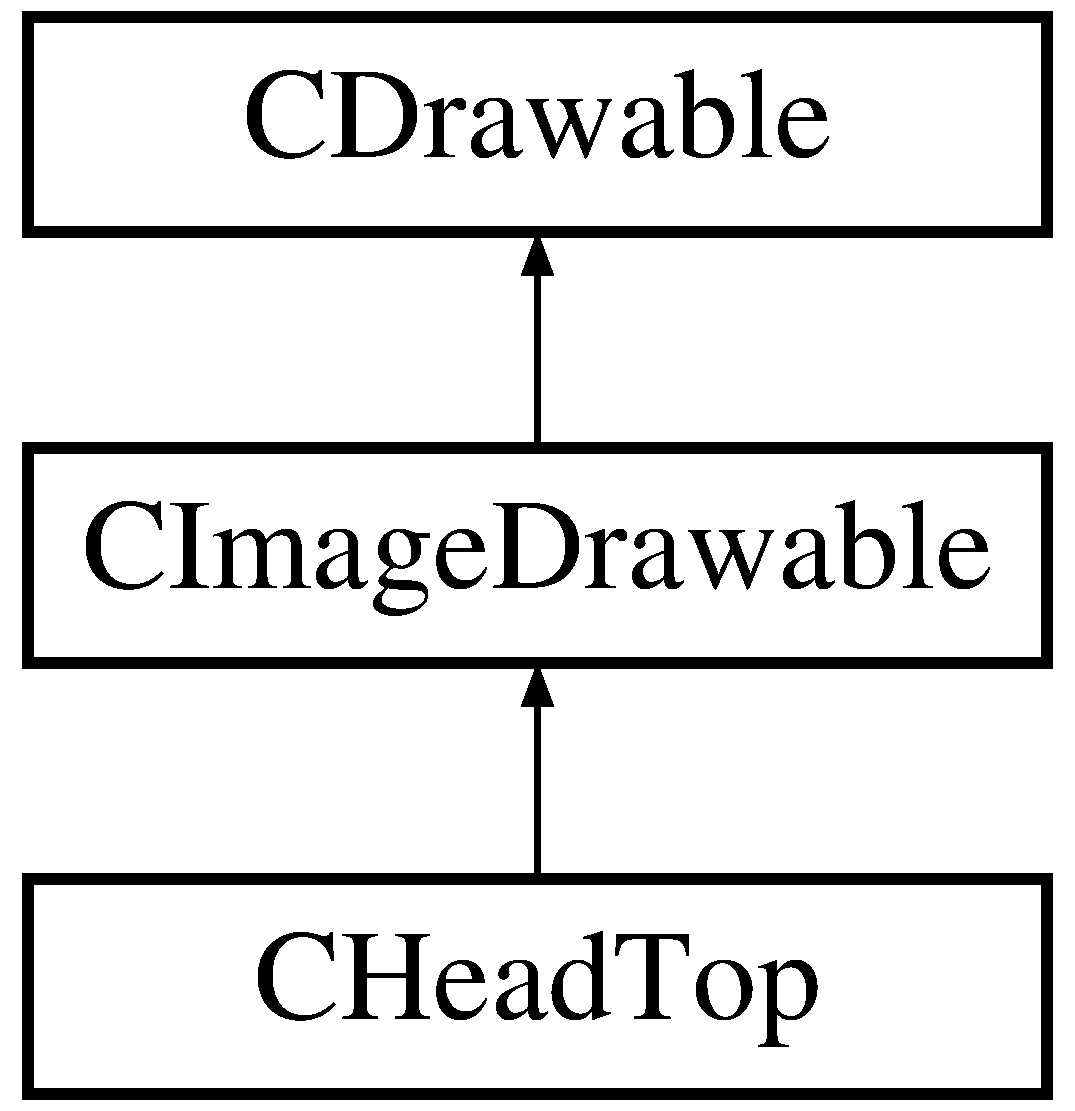
\includegraphics[height=3.000000cm]{class_c_head_top}
\end{center}
\end{figure}
\subsection*{Public Member Functions}
\begin{DoxyCompactItemize}
\item 
\hypertarget{class_c_head_top_a54fab18f42f367ff9cfdf73537ada62f}{\hyperlink{class_c_head_top_a54fab18f42f367ff9cfdf73537ada62f}{C\+Head\+Top} ()=delete}\label{class_c_head_top_a54fab18f42f367ff9cfdf73537ada62f}

\begin{DoxyCompactList}\small\item\em Default constructor disabled. \end{DoxyCompactList}\item 
\hypertarget{class_c_head_top_a574b5950dff9f90de01219437f475cb9}{\hyperlink{class_c_head_top_a574b5950dff9f90de01219437f475cb9}{C\+Head\+Top} (const \hyperlink{class_c_head_top}{C\+Head\+Top} \&)=delete}\label{class_c_head_top_a574b5950dff9f90de01219437f475cb9}

\begin{DoxyCompactList}\small\item\em Copy constructor disabled. \end{DoxyCompactList}\item 
\hypertarget{class_c_head_top_aeb3522f283f90cb48b7b6a7ed6243aeb}{void \hyperlink{class_c_head_top_aeb3522f283f90cb48b7b6a7ed6243aeb}{operator=} (const \hyperlink{class_c_head_top}{C\+Head\+Top} \&)=delete}\label{class_c_head_top_aeb3522f283f90cb48b7b6a7ed6243aeb}

\begin{DoxyCompactList}\small\item\em Assignment operator disabled. \end{DoxyCompactList}\item 
\hyperlink{class_c_head_top_a31333179dc1836d6ae5b9636b215b66b}{C\+Head\+Top} (const std\+::wstring \&name, const std\+::wstring \&filename)
\begin{DoxyCompactList}\small\item\em constructor \end{DoxyCompactList}\item 
void \hyperlink{class_c_head_top_aa77d9fa703079ee68a4e4e8e3c816932}{Draw} (Gdiplus\+::\+Graphics $\ast$graphics)
\begin{DoxyCompactList}\small\item\em Drawing. \end{DoxyCompactList}\item 
Gdiplus\+::\+Point \hyperlink{class_c_head_top_a631542f2cc871fa17542b3253dc6ab73}{Transform\+Point} (Gdiplus\+::\+Point p)
\begin{DoxyCompactList}\small\item\em transform \end{DoxyCompactList}\item 
\hypertarget{class_c_head_top_a64697c81bc0100f66aa661a8bc430fa9}{virtual \hyperlink{class_c_head_top_a64697c81bc0100f66aa661a8bc430fa9}{$\sim$\+C\+Head\+Top} ()}\label{class_c_head_top_a64697c81bc0100f66aa661a8bc430fa9}

\begin{DoxyCompactList}\small\item\em destructor \end{DoxyCompactList}\item 
bool \hyperlink{class_c_head_top_a38d98789668f640fa3bbb8352fb54c49}{Is\+Movable} () override
\begin{DoxyCompactList}\small\item\em Moveable override. \end{DoxyCompactList}\end{DoxyCompactItemize}
\subsection*{Additional Inherited Members}


\subsection{Detailed Description}
the head

head drawable 

\subsection{Constructor \& Destructor Documentation}
\hypertarget{class_c_head_top_a31333179dc1836d6ae5b9636b215b66b}{\index{C\+Head\+Top@{C\+Head\+Top}!C\+Head\+Top@{C\+Head\+Top}}
\index{C\+Head\+Top@{C\+Head\+Top}!C\+Head\+Top@{C\+Head\+Top}}
\subsubsection[{C\+Head\+Top}]{\setlength{\rightskip}{0pt plus 5cm}C\+Head\+Top\+::\+C\+Head\+Top (
\begin{DoxyParamCaption}
\item[{const std\+::wstring \&}]{name, }
\item[{const std\+::wstring \&}]{filename}
\end{DoxyParamCaption}
)}}\label{class_c_head_top_a31333179dc1836d6ae5b9636b215b66b}


constructor 


\begin{DoxyParams}{Parameters}
{\em name} & is name \\
\hline
{\em filename} & for opening \\
\hline
\end{DoxyParams}


\subsection{Member Function Documentation}
\hypertarget{class_c_head_top_aa77d9fa703079ee68a4e4e8e3c816932}{\index{C\+Head\+Top@{C\+Head\+Top}!Draw@{Draw}}
\index{Draw@{Draw}!C\+Head\+Top@{C\+Head\+Top}}
\subsubsection[{Draw}]{\setlength{\rightskip}{0pt plus 5cm}void C\+Head\+Top\+::\+Draw (
\begin{DoxyParamCaption}
\item[{Gdiplus\+::\+Graphics $\ast$}]{graphics}
\end{DoxyParamCaption}
)\hspace{0.3cm}{\ttfamily [virtual]}}}\label{class_c_head_top_aa77d9fa703079ee68a4e4e8e3c816932}


Drawing. 


\begin{DoxyParams}{Parameters}
{\em graphics} & for drawing\\
\hline
\end{DoxyParams}
Draw the image drawable 
\begin{DoxyParams}{Parameters}
{\em graphics} & Graphics context to draw on \\
\hline
\end{DoxyParams}
T\+H\+I\+S S\+E\+C\+T\+I\+O\+N I\+S T\+O S\+T\+I\+L\+L D\+R\+A\+W H\+E\+A\+D 

Implements \hyperlink{class_c_drawable_a9b6a9920a75d88d9ae321997495eaec7}{C\+Drawable}.

\hypertarget{class_c_head_top_a38d98789668f640fa3bbb8352fb54c49}{\index{C\+Head\+Top@{C\+Head\+Top}!Is\+Movable@{Is\+Movable}}
\index{Is\+Movable@{Is\+Movable}!C\+Head\+Top@{C\+Head\+Top}}
\subsubsection[{Is\+Movable}]{\setlength{\rightskip}{0pt plus 5cm}bool C\+Head\+Top\+::\+Is\+Movable (
\begin{DoxyParamCaption}
{}
\end{DoxyParamCaption}
)\hspace{0.3cm}{\ttfamily [inline]}, {\ttfamily [override]}, {\ttfamily [virtual]}}}\label{class_c_head_top_a38d98789668f640fa3bbb8352fb54c49}


Moveable override. 

\begin{DoxyReturn}{Returns}
true always 
\end{DoxyReturn}


Reimplemented from \hyperlink{class_c_drawable_ac9f03cfc58aed75fb52cd69c71e7b6e0}{C\+Drawable}.

\hypertarget{class_c_head_top_a631542f2cc871fa17542b3253dc6ab73}{\index{C\+Head\+Top@{C\+Head\+Top}!Transform\+Point@{Transform\+Point}}
\index{Transform\+Point@{Transform\+Point}!C\+Head\+Top@{C\+Head\+Top}}
\subsubsection[{Transform\+Point}]{\setlength{\rightskip}{0pt plus 5cm}Gdiplus\+::\+Point C\+Head\+Top\+::\+Transform\+Point (
\begin{DoxyParamCaption}
\item[{Gdiplus\+::\+Point}]{p}
\end{DoxyParamCaption}
)}}\label{class_c_head_top_a631542f2cc871fa17542b3253dc6ab73}


transform 


\begin{DoxyParams}{Parameters}
{\em p} & is the point to transform\\
\hline
\end{DoxyParams}
Transform a point from a location on the bitmap to a location on the screen. 
\begin{DoxyParams}{Parameters}
{\em p} & Point to transform \\
\hline
\end{DoxyParams}
\begin{DoxyReturn}{Returns}
Transformed point 
\end{DoxyReturn}


The documentation for this class was generated from the following files\+:\begin{DoxyCompactItemize}
\item 
\hyperlink{_head_top_8h}{Head\+Top.\+h}\item 
Head\+Top.\+cpp\end{DoxyCompactItemize}

\hypertarget{class_c_image_drawable}{\section{C\+Image\+Drawable Class Reference}
\label{class_c_image_drawable}\index{C\+Image\+Drawable@{C\+Image\+Drawable}}
}


{\ttfamily \#include $<$Image\+Drawable.\+h$>$}

Inheritance diagram for C\+Image\+Drawable\+:\begin{figure}[H]
\begin{center}
\leavevmode
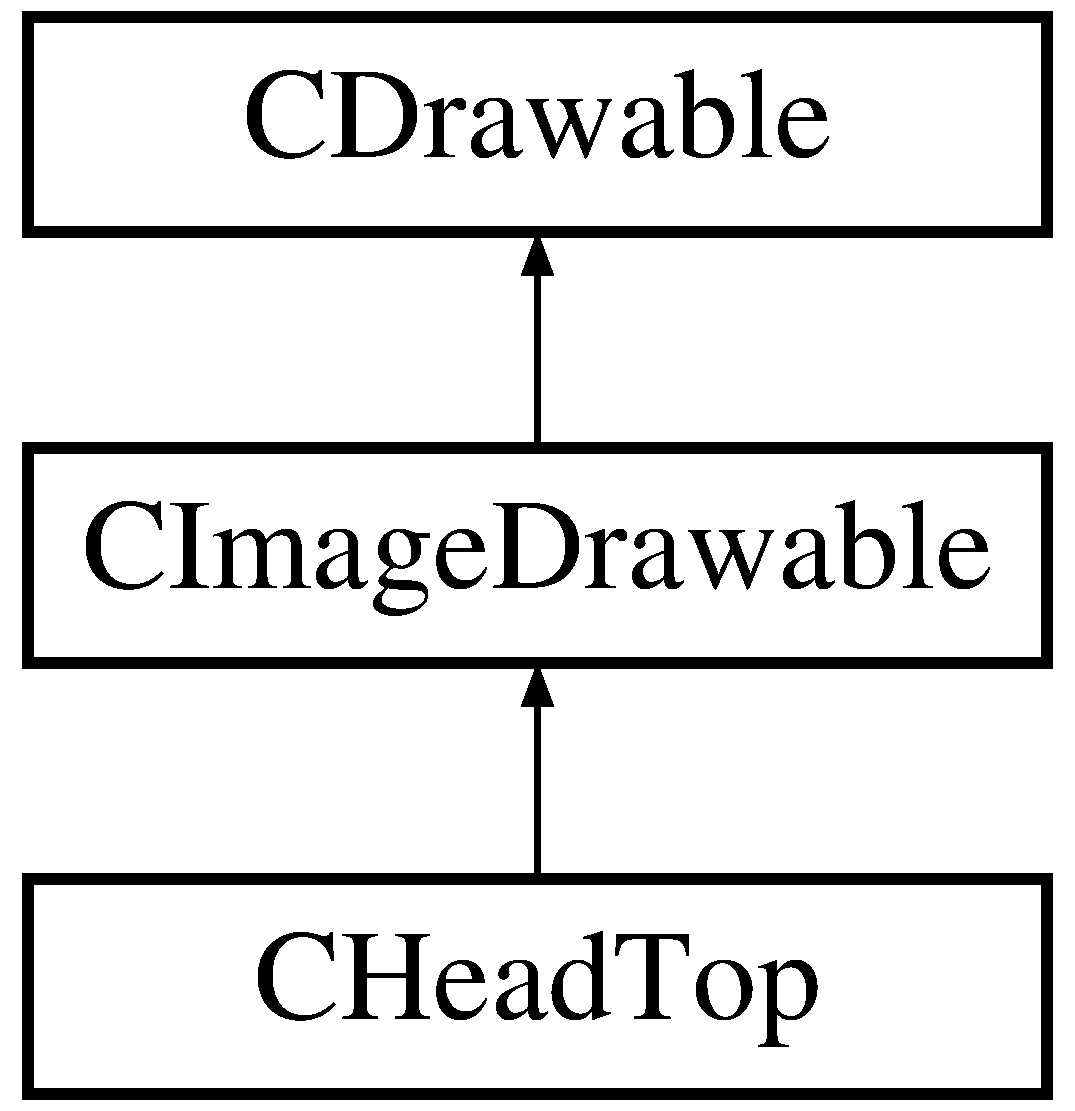
\includegraphics[height=3.000000cm]{class_c_image_drawable}
\end{center}
\end{figure}
\subsection*{Public Member Functions}
\begin{DoxyCompactItemize}
\item 
\hypertarget{class_c_image_drawable_a0af067ad80ece0bea046dded19c5b9d4}{\hyperlink{class_c_image_drawable_a0af067ad80ece0bea046dded19c5b9d4}{C\+Image\+Drawable} ()=delete}\label{class_c_image_drawable_a0af067ad80ece0bea046dded19c5b9d4}

\begin{DoxyCompactList}\small\item\em Default constructor disabled. \end{DoxyCompactList}\item 
\hypertarget{class_c_image_drawable_a2955356238c638373d39ed99c5422cf3}{\hyperlink{class_c_image_drawable_a2955356238c638373d39ed99c5422cf3}{C\+Image\+Drawable} (const \hyperlink{class_c_image_drawable}{C\+Image\+Drawable} \&)=delete}\label{class_c_image_drawable_a2955356238c638373d39ed99c5422cf3}

\begin{DoxyCompactList}\small\item\em Copy constructor disabled. \end{DoxyCompactList}\item 
\hypertarget{class_c_image_drawable_a717129f6ce9e9fa5d9a512a85a33a8b1}{void \hyperlink{class_c_image_drawable_a717129f6ce9e9fa5d9a512a85a33a8b1}{operator=} (const \hyperlink{class_c_image_drawable}{C\+Image\+Drawable} \&)=delete}\label{class_c_image_drawable_a717129f6ce9e9fa5d9a512a85a33a8b1}

\begin{DoxyCompactList}\small\item\em Assignment operator disabled. \end{DoxyCompactList}\item 
Gdiplus\+::\+Point \hyperlink{class_c_image_drawable_adaf3918b7eafe6c3db2c73ffa317f114}{Get\+Center} ()
\item 
void \hyperlink{class_c_image_drawable_a11c2376e3516076e7e737a5a266f1c49}{Set\+Center} (Gdiplus\+::\+Point center)
\item 
virtual \hyperlink{class_c_image_drawable_a4ecb6e494ba125a2d503bfff1260c2fe}{$\sim$\+C\+Image\+Drawable} ()
\item 
\hyperlink{class_c_image_drawable_a0a036788340edfd1765ae6a05cee31a0}{C\+Image\+Drawable} (const std\+::wstring \&name, const std\+::wstring \&filename)
\item 
void \hyperlink{class_c_image_drawable_abf591e6f5e92537119ab745eba054bd1}{Draw} (Gdiplus\+::\+Graphics $\ast$graphics)
\item 
bool \hyperlink{class_c_image_drawable_ac9f173d9fcb21dbb45f4cbf4593a6984}{Hit\+Test} (Gdiplus\+::\+Point pos)
\end{DoxyCompactItemize}
\subsection*{Protected Attributes}
\begin{DoxyCompactItemize}
\item 
\hypertarget{class_c_image_drawable_ae55a012a4867007fc409db9d71476c71}{std\+::unique\+\_\+ptr$<$ Gdiplus\+::\+Bitmap $>$ \hyperlink{class_c_image_drawable_ae55a012a4867007fc409db9d71476c71}{m\+Image}}\label{class_c_image_drawable_ae55a012a4867007fc409db9d71476c71}

\begin{DoxyCompactList}\small\item\em The image for this drawable. \end{DoxyCompactList}\end{DoxyCompactItemize}
\subsection*{Additional Inherited Members}


\subsection{Detailed Description}
the image drawable

Inherited from drawable 

\subsection{Constructor \& Destructor Documentation}
\hypertarget{class_c_image_drawable_a4ecb6e494ba125a2d503bfff1260c2fe}{\index{C\+Image\+Drawable@{C\+Image\+Drawable}!````~C\+Image\+Drawable@{$\sim$\+C\+Image\+Drawable}}
\index{````~C\+Image\+Drawable@{$\sim$\+C\+Image\+Drawable}!C\+Image\+Drawable@{C\+Image\+Drawable}}
\subsubsection[{$\sim$\+C\+Image\+Drawable}]{\setlength{\rightskip}{0pt plus 5cm}C\+Image\+Drawable\+::$\sim$\+C\+Image\+Drawable (
\begin{DoxyParamCaption}
{}
\end{DoxyParamCaption}
)\hspace{0.3cm}{\ttfamily [virtual]}}}\label{class_c_image_drawable_a4ecb6e494ba125a2d503bfff1260c2fe}
Deconstructor \hypertarget{class_c_image_drawable_a0a036788340edfd1765ae6a05cee31a0}{\index{C\+Image\+Drawable@{C\+Image\+Drawable}!C\+Image\+Drawable@{C\+Image\+Drawable}}
\index{C\+Image\+Drawable@{C\+Image\+Drawable}!C\+Image\+Drawable@{C\+Image\+Drawable}}
\subsubsection[{C\+Image\+Drawable}]{\setlength{\rightskip}{0pt plus 5cm}C\+Image\+Drawable\+::\+C\+Image\+Drawable (
\begin{DoxyParamCaption}
\item[{const std\+::wstring \&}]{name, }
\item[{const std\+::wstring \&}]{filename}
\end{DoxyParamCaption}
)}}\label{class_c_image_drawable_a0a036788340edfd1765ae6a05cee31a0}
cons 
\begin{DoxyParams}{Parameters}
{\em name} & is name \\
\hline
{\em filename} & for constructor\\
\hline
\end{DoxyParams}
Constructor 
\begin{DoxyParams}{Parameters}
{\em name} & The drawable name \\
\hline
{\em filename} & The filename for the image \\
\hline
\end{DoxyParams}


\subsection{Member Function Documentation}
\hypertarget{class_c_image_drawable_abf591e6f5e92537119ab745eba054bd1}{\index{C\+Image\+Drawable@{C\+Image\+Drawable}!Draw@{Draw}}
\index{Draw@{Draw}!C\+Image\+Drawable@{C\+Image\+Drawable}}
\subsubsection[{Draw}]{\setlength{\rightskip}{0pt plus 5cm}void C\+Image\+Drawable\+::\+Draw (
\begin{DoxyParamCaption}
\item[{Gdiplus\+::\+Graphics $\ast$}]{graphics}
\end{DoxyParamCaption}
)\hspace{0.3cm}{\ttfamily [virtual]}}}\label{class_c_image_drawable_abf591e6f5e92537119ab745eba054bd1}
Draw 
\begin{DoxyParams}{Parameters}
{\em graphics} & object for drawing.\\
\hline
\end{DoxyParams}
Draw the image drawable 
\begin{DoxyParams}{Parameters}
{\em graphics} & Graphics context to draw on \\
\hline
\end{DoxyParams}


Implements \hyperlink{class_c_drawable_a9b6a9920a75d88d9ae321997495eaec7}{C\+Drawable}.

\hypertarget{class_c_image_drawable_adaf3918b7eafe6c3db2c73ffa317f114}{\index{C\+Image\+Drawable@{C\+Image\+Drawable}!Get\+Center@{Get\+Center}}
\index{Get\+Center@{Get\+Center}!C\+Image\+Drawable@{C\+Image\+Drawable}}
\subsubsection[{Get\+Center}]{\setlength{\rightskip}{0pt plus 5cm}Gdiplus\+::\+Point C\+Image\+Drawable\+::\+Get\+Center (
\begin{DoxyParamCaption}
{}
\end{DoxyParamCaption}
)\hspace{0.3cm}{\ttfamily [inline]}}}\label{class_c_image_drawable_adaf3918b7eafe6c3db2c73ffa317f114}
center \begin{DoxyReturn}{Returns}
m\+Center 
\end{DoxyReturn}
\hypertarget{class_c_image_drawable_ac9f173d9fcb21dbb45f4cbf4593a6984}{\index{C\+Image\+Drawable@{C\+Image\+Drawable}!Hit\+Test@{Hit\+Test}}
\index{Hit\+Test@{Hit\+Test}!C\+Image\+Drawable@{C\+Image\+Drawable}}
\subsubsection[{Hit\+Test}]{\setlength{\rightskip}{0pt plus 5cm}bool C\+Image\+Drawable\+::\+Hit\+Test (
\begin{DoxyParamCaption}
\item[{Gdiplus\+::\+Point}]{pos}
\end{DoxyParamCaption}
)\hspace{0.3cm}{\ttfamily [virtual]}}}\label{class_c_image_drawable_ac9f173d9fcb21dbb45f4cbf4593a6984}
cons 
\begin{DoxyParams}{Parameters}
{\em pos} & position\\
\hline
\end{DoxyParams}
Test to see if we clicked on the image. 
\begin{DoxyParams}{Parameters}
{\em pos} & Position to test \\
\hline
\end{DoxyParams}
\begin{DoxyReturn}{Returns}
True if clicked on 
\end{DoxyReturn}


Implements \hyperlink{class_c_drawable_af715bc2e79788b2a44a74ad70b181544}{C\+Drawable}.

\hypertarget{class_c_image_drawable_a11c2376e3516076e7e737a5a266f1c49}{\index{C\+Image\+Drawable@{C\+Image\+Drawable}!Set\+Center@{Set\+Center}}
\index{Set\+Center@{Set\+Center}!C\+Image\+Drawable@{C\+Image\+Drawable}}
\subsubsection[{Set\+Center}]{\setlength{\rightskip}{0pt plus 5cm}void C\+Image\+Drawable\+::\+Set\+Center (
\begin{DoxyParamCaption}
\item[{Gdiplus\+::\+Point}]{center}
\end{DoxyParamCaption}
)\hspace{0.3cm}{\ttfamily [inline]}}}\label{class_c_image_drawable_a11c2376e3516076e7e737a5a266f1c49}
Sets center 
\begin{DoxyParams}{Parameters}
{\em center} & is m variable \\
\hline
\end{DoxyParams}


The documentation for this class was generated from the following files\+:\begin{DoxyCompactItemize}
\item 
\hyperlink{_image_drawable_8h}{Image\+Drawable.\+h}\item 
Image\+Drawable.\+cpp\end{DoxyCompactItemize}

\hypertarget{class_c_main_frame}{\section{C\+Main\+Frame Class Reference}
\label{class_c_main_frame}\index{C\+Main\+Frame@{C\+Main\+Frame}}
}


{\ttfamily \#include $<$Main\+Frm.\+h$>$}

Inheritance diagram for C\+Main\+Frame\+:\begin{figure}[H]
\begin{center}
\leavevmode
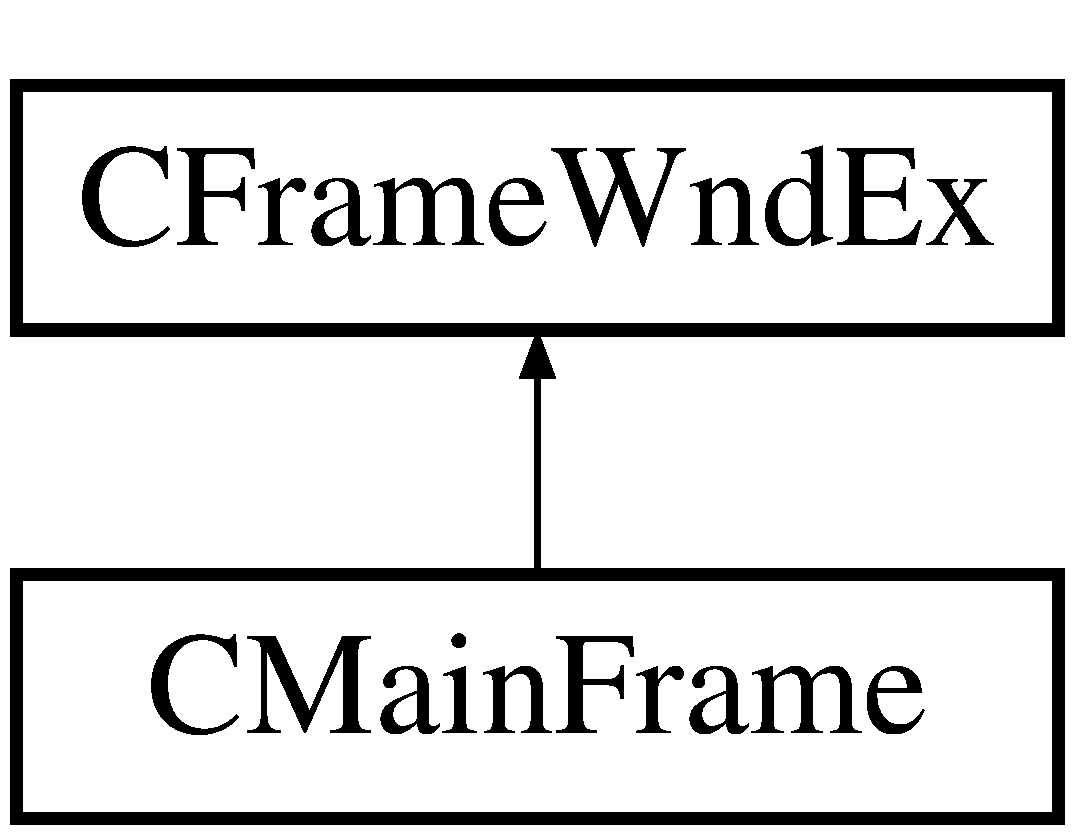
\includegraphics[height=2.000000cm]{class_c_main_frame}
\end{center}
\end{figure}
\subsection*{Public Types}
\begin{DoxyCompactItemize}
\item 
enum \hyperlink{class_c_main_frame_a89722c82d82f95a761772a8dd9755b7b}{Motion\+Modes} \{ {\bfseries Move}, 
{\bfseries Rotate}
 \}
\end{DoxyCompactItemize}
\subsection*{Public Member Functions}
\begin{DoxyCompactItemize}
\item 
\hyperlink{class_c_main_frame_af3e997aeae4148d2aaa4a1e1ae7bdd53}{C\+Main\+Frame} ()
\item 
\hyperlink{class_c_main_frame_a89722c82d82f95a761772a8dd9755b7b}{Motion\+Modes} \hyperlink{class_c_main_frame_a76c571ab75752dba8049e08f5e4ac920}{Get\+Mode} () const 
\item 
\hypertarget{class_c_main_frame_a549bf677c955c2898c3c683321633c16}{virtual B\+O\+O\+L {\bfseries Pre\+Create\+Window} (C\+R\+E\+A\+T\+E\+S\+T\+R\+U\+C\+T \&cs)}\label{class_c_main_frame_a549bf677c955c2898c3c683321633c16}

\item 
\hypertarget{class_c_main_frame_ade959eb0bab719bf06bb9b18ee407101}{virtual B\+O\+O\+L {\bfseries On\+Cmd\+Msg} (U\+I\+N\+T n\+I\+D, int n\+Code, void $\ast$p\+Extra, A\+F\+X\+\_\+\+C\+M\+D\+H\+A\+N\+D\+L\+E\+R\+I\+N\+F\+O $\ast$p\+Handler\+Info)}\label{class_c_main_frame_ade959eb0bab719bf06bb9b18ee407101}

\item 
virtual \hyperlink{class_c_main_frame_a8ae555f23fdf97edb4feb4d3e1bfa4ee}{$\sim$\+C\+Main\+Frame} ()
\item 
afx\+\_\+msg void \hyperlink{class_c_main_frame_adf171bf1f2c6f10cc85dbe8db3fc93f7}{On\+Size} (U\+I\+N\+T n\+Type, int cx, int cy)
\item 
afx\+\_\+msg B\+O\+O\+L \hyperlink{class_c_main_frame_a53a97f2229c5765329b2b59a21a54b0d}{On\+Erase\+Bkgnd} (C\+D\+C $\ast$p\+D\+C)
\item 
afx\+\_\+msg void \hyperlink{class_c_main_frame_af07c2610f9f5631e7eb7374d10d5fdd3}{On\+Edit\+Move} ()
\item 
afx\+\_\+msg void \hyperlink{class_c_main_frame_aadc40c4ab290da2368f6b87443f5ffbc}{On\+Update\+Edit\+Move} (C\+Cmd\+U\+I $\ast$p\+Cmd\+U\+I)
\item 
afx\+\_\+msg void \hyperlink{class_c_main_frame_a00f10667f35de1fa6693c1bea941d878}{On\+Edit\+Rotate} ()
\item 
afx\+\_\+msg void \hyperlink{class_c_main_frame_af098b8129775d1b5fb47fcaaabce8c01}{On\+Update\+Edit\+Rotate} (C\+Cmd\+U\+I $\ast$p\+Cmd\+U\+I)
\end{DoxyCompactItemize}
\subsection*{Protected Member Functions}
\begin{DoxyCompactItemize}
\item 
afx\+\_\+msg int \hyperlink{class_c_main_frame_a48666466fd37412fcaeff75c3b12e0ed}{On\+Create} (L\+P\+C\+R\+E\+A\+T\+E\+S\+T\+R\+U\+C\+T lp\+Create\+Struct)
\item 
afx\+\_\+msg void \hyperlink{class_c_main_frame_adc353a3d1fc497fbc009b6d9e6914a82}{On\+Set\+Focus} (C\+Wnd $\ast$p\+Old\+Wnd)
\item 
virtual B\+O\+O\+L \hyperlink{class_c_main_frame_ac863d694fd3637d492ef97396defbd8e}{On\+Create\+Client} (L\+P\+C\+R\+E\+A\+T\+E\+S\+T\+R\+U\+C\+T lpcs, C\+Create\+Context $\ast$p\+Context)
\end{DoxyCompactItemize}
\subsection*{Protected Attributes}
\begin{DoxyCompactItemize}
\item 
\hypertarget{class_c_main_frame_ac8558942627d1502b5095e736840a1f3}{C\+M\+F\+C\+Tool\+Bar {\bfseries m\+\_\+wnd\+Tool\+Bar}}\label{class_c_main_frame_ac8558942627d1502b5095e736840a1f3}

\item 
\hypertarget{class_c_main_frame_a5842bded00e9137fbbf77343b99863be}{C\+M\+F\+C\+Status\+Bar \hyperlink{class_c_main_frame_a5842bded00e9137fbbf77343b99863be}{m\+\_\+wnd\+Status\+Bar}}\label{class_c_main_frame_a5842bded00e9137fbbf77343b99863be}

\begin{DoxyCompactList}\small\item\em toolbar \end{DoxyCompactList}\item 
\hypertarget{class_c_main_frame_a1d68466db594c4bebf41f707bc0a0647}{C\+Splitter\+Wnd \hyperlink{class_c_main_frame_a1d68466db594c4bebf41f707bc0a0647}{m\+Wnd\+Splitter}}\label{class_c_main_frame_a1d68466db594c4bebf41f707bc0a0647}

\begin{DoxyCompactList}\small\item\em status bad \end{DoxyCompactList}\item 
std\+::shared\+\_\+ptr$<$ \hyperlink{class_c_picture}{C\+Picture} $>$ \hyperlink{class_c_main_frame_aee7250305e9d4adb463024fe090a2c10}{m\+Picture}
\begin{DoxyCompactList}\small\item\em The picture object we are viewing/editing. \end{DoxyCompactList}\end{DoxyCompactItemize}


\subsection{Detailed Description}
Program main frame 

\subsection{Member Enumeration Documentation}
\hypertarget{class_c_main_frame_a89722c82d82f95a761772a8dd9755b7b}{\index{C\+Main\+Frame@{C\+Main\+Frame}!Motion\+Modes@{Motion\+Modes}}
\index{Motion\+Modes@{Motion\+Modes}!C\+Main\+Frame@{C\+Main\+Frame}}
\subsubsection[{Motion\+Modes}]{\setlength{\rightskip}{0pt plus 5cm}enum {\bf C\+Main\+Frame\+::\+Motion\+Modes}}}\label{class_c_main_frame_a89722c82d82f95a761772a8dd9755b7b}
Enumerations for the possible manipulation modes 

\subsection{Constructor \& Destructor Documentation}
\hypertarget{class_c_main_frame_af3e997aeae4148d2aaa4a1e1ae7bdd53}{\index{C\+Main\+Frame@{C\+Main\+Frame}!C\+Main\+Frame@{C\+Main\+Frame}}
\index{C\+Main\+Frame@{C\+Main\+Frame}!C\+Main\+Frame@{C\+Main\+Frame}}
\subsubsection[{C\+Main\+Frame}]{\setlength{\rightskip}{0pt plus 5cm}C\+Main\+Frame\+::\+C\+Main\+Frame (
\begin{DoxyParamCaption}
{}
\end{DoxyParamCaption}
)}}\label{class_c_main_frame_af3e997aeae4148d2aaa4a1e1ae7bdd53}
Constructor \hypertarget{class_c_main_frame_a8ae555f23fdf97edb4feb4d3e1bfa4ee}{\index{C\+Main\+Frame@{C\+Main\+Frame}!````~C\+Main\+Frame@{$\sim$\+C\+Main\+Frame}}
\index{````~C\+Main\+Frame@{$\sim$\+C\+Main\+Frame}!C\+Main\+Frame@{C\+Main\+Frame}}
\subsubsection[{$\sim$\+C\+Main\+Frame}]{\setlength{\rightskip}{0pt plus 5cm}C\+Main\+Frame\+::$\sim$\+C\+Main\+Frame (
\begin{DoxyParamCaption}
{}
\end{DoxyParamCaption}
)\hspace{0.3cm}{\ttfamily [virtual]}}}\label{class_c_main_frame_a8ae555f23fdf97edb4feb4d3e1bfa4ee}
Destructor 

\subsection{Member Function Documentation}
\hypertarget{class_c_main_frame_a76c571ab75752dba8049e08f5e4ac920}{\index{C\+Main\+Frame@{C\+Main\+Frame}!Get\+Mode@{Get\+Mode}}
\index{Get\+Mode@{Get\+Mode}!C\+Main\+Frame@{C\+Main\+Frame}}
\subsubsection[{Get\+Mode}]{\setlength{\rightskip}{0pt plus 5cm}{\bf Motion\+Modes} C\+Main\+Frame\+::\+Get\+Mode (
\begin{DoxyParamCaption}
{}
\end{DoxyParamCaption}
) const\hspace{0.3cm}{\ttfamily [inline]}}}\label{class_c_main_frame_a76c571ab75752dba8049e08f5e4ac920}
The selected manipulation mode \begin{DoxyReturn}{Returns}
Currently selected manipulation mode 
\end{DoxyReturn}
\hypertarget{class_c_main_frame_a48666466fd37412fcaeff75c3b12e0ed}{\index{C\+Main\+Frame@{C\+Main\+Frame}!On\+Create@{On\+Create}}
\index{On\+Create@{On\+Create}!C\+Main\+Frame@{C\+Main\+Frame}}
\subsubsection[{On\+Create}]{\setlength{\rightskip}{0pt plus 5cm}int C\+Main\+Frame\+::\+On\+Create (
\begin{DoxyParamCaption}
\item[{L\+P\+C\+R\+E\+A\+T\+E\+S\+T\+R\+U\+C\+T}]{lp\+Create\+Struct}
\end{DoxyParamCaption}
)\hspace{0.3cm}{\ttfamily [protected]}}}\label{class_c_main_frame_a48666466fd37412fcaeff75c3b12e0ed}
create 
\begin{DoxyParams}{Parameters}
{\em lp\+Create\+Struct} & is old \\
\hline
\end{DoxyParams}
\hypertarget{class_c_main_frame_ac863d694fd3637d492ef97396defbd8e}{\index{C\+Main\+Frame@{C\+Main\+Frame}!On\+Create\+Client@{On\+Create\+Client}}
\index{On\+Create\+Client@{On\+Create\+Client}!C\+Main\+Frame@{C\+Main\+Frame}}
\subsubsection[{On\+Create\+Client}]{\setlength{\rightskip}{0pt plus 5cm}B\+O\+O\+L C\+Main\+Frame\+::\+On\+Create\+Client (
\begin{DoxyParamCaption}
\item[{L\+P\+C\+R\+E\+A\+T\+E\+S\+T\+R\+U\+C\+T}]{lpcs, }
\item[{C\+Create\+Context $\ast$}]{p\+Context}
\end{DoxyParamCaption}
)\hspace{0.3cm}{\ttfamily [protected]}, {\ttfamily [virtual]}}}\label{class_c_main_frame_ac863d694fd3637d492ef97396defbd8e}
Oncreate client 
\begin{DoxyParams}{Parameters}
{\em lpcs} & is good \\
\hline
{\em p\+Context} & is context \\
\hline
\end{DoxyParams}
\hypertarget{class_c_main_frame_af07c2610f9f5631e7eb7374d10d5fdd3}{\index{C\+Main\+Frame@{C\+Main\+Frame}!On\+Edit\+Move@{On\+Edit\+Move}}
\index{On\+Edit\+Move@{On\+Edit\+Move}!C\+Main\+Frame@{C\+Main\+Frame}}
\subsubsection[{On\+Edit\+Move}]{\setlength{\rightskip}{0pt plus 5cm}void C\+Main\+Frame\+::\+On\+Edit\+Move (
\begin{DoxyParamCaption}
{}
\end{DoxyParamCaption}
)}}\label{class_c_main_frame_af07c2610f9f5631e7eb7374d10d5fdd3}
Handle the Edit$>$Mode menu option \hypertarget{class_c_main_frame_a00f10667f35de1fa6693c1bea941d878}{\index{C\+Main\+Frame@{C\+Main\+Frame}!On\+Edit\+Rotate@{On\+Edit\+Rotate}}
\index{On\+Edit\+Rotate@{On\+Edit\+Rotate}!C\+Main\+Frame@{C\+Main\+Frame}}
\subsubsection[{On\+Edit\+Rotate}]{\setlength{\rightskip}{0pt plus 5cm}void C\+Main\+Frame\+::\+On\+Edit\+Rotate (
\begin{DoxyParamCaption}
{}
\end{DoxyParamCaption}
)}}\label{class_c_main_frame_a00f10667f35de1fa6693c1bea941d878}
Handle the Edit$>$Rotate menu option \hypertarget{class_c_main_frame_a53a97f2229c5765329b2b59a21a54b0d}{\index{C\+Main\+Frame@{C\+Main\+Frame}!On\+Erase\+Bkgnd@{On\+Erase\+Bkgnd}}
\index{On\+Erase\+Bkgnd@{On\+Erase\+Bkgnd}!C\+Main\+Frame@{C\+Main\+Frame}}
\subsubsection[{On\+Erase\+Bkgnd}]{\setlength{\rightskip}{0pt plus 5cm}B\+O\+O\+L C\+Main\+Frame\+::\+On\+Erase\+Bkgnd (
\begin{DoxyParamCaption}
\item[{C\+D\+C $\ast$}]{p\+D\+C}
\end{DoxyParamCaption}
)}}\label{class_c_main_frame_a53a97f2229c5765329b2b59a21a54b0d}
Called to erase the background. Disabled so we don't get flicker 
\begin{DoxyParams}{Parameters}
{\em p\+D\+C} & A device context \\
\hline
\end{DoxyParams}
\begin{DoxyReturn}{Returns}
F\+A\+L\+S\+E 
\end{DoxyReturn}
\hypertarget{class_c_main_frame_adc353a3d1fc497fbc009b6d9e6914a82}{\index{C\+Main\+Frame@{C\+Main\+Frame}!On\+Set\+Focus@{On\+Set\+Focus}}
\index{On\+Set\+Focus@{On\+Set\+Focus}!C\+Main\+Frame@{C\+Main\+Frame}}
\subsubsection[{On\+Set\+Focus}]{\setlength{\rightskip}{0pt plus 5cm}void C\+Main\+Frame\+::\+On\+Set\+Focus (
\begin{DoxyParamCaption}
\item[{C\+Wnd $\ast$}]{p\+Old\+Wnd}
\end{DoxyParamCaption}
)\hspace{0.3cm}{\ttfamily [protected]}}}\label{class_c_main_frame_adc353a3d1fc497fbc009b6d9e6914a82}
set focus 
\begin{DoxyParams}{Parameters}
{\em p\+Old\+Wnd} & is old \\
\hline
\end{DoxyParams}
\hypertarget{class_c_main_frame_adf171bf1f2c6f10cc85dbe8db3fc93f7}{\index{C\+Main\+Frame@{C\+Main\+Frame}!On\+Size@{On\+Size}}
\index{On\+Size@{On\+Size}!C\+Main\+Frame@{C\+Main\+Frame}}
\subsubsection[{On\+Size}]{\setlength{\rightskip}{0pt plus 5cm}void C\+Main\+Frame\+::\+On\+Size (
\begin{DoxyParamCaption}
\item[{U\+I\+N\+T}]{n\+Type, }
\item[{int}]{cx, }
\item[{int}]{cy}
\end{DoxyParamCaption}
)}}\label{class_c_main_frame_adf171bf1f2c6f10cc85dbe8db3fc93f7}
Handle a Size request from Windows

This function ensures the child windows are the correct size on the screen after the main window is resized 
\begin{DoxyParams}{Parameters}
{\em n\+Type} & Type of resizing message \\
\hline
{\em cx} & The new width \\
\hline
{\em cy} & The new height \\
\hline
\end{DoxyParams}
\hypertarget{class_c_main_frame_aadc40c4ab290da2368f6b87443f5ffbc}{\index{C\+Main\+Frame@{C\+Main\+Frame}!On\+Update\+Edit\+Move@{On\+Update\+Edit\+Move}}
\index{On\+Update\+Edit\+Move@{On\+Update\+Edit\+Move}!C\+Main\+Frame@{C\+Main\+Frame}}
\subsubsection[{On\+Update\+Edit\+Move}]{\setlength{\rightskip}{0pt plus 5cm}void C\+Main\+Frame\+::\+On\+Update\+Edit\+Move (
\begin{DoxyParamCaption}
\item[{C\+Cmd\+U\+I $\ast$}]{p\+Cmd\+U\+I}
\end{DoxyParamCaption}
)}}\label{class_c_main_frame_aadc40c4ab290da2368f6b87443f5ffbc}
Update the menu for Edit$>$Move 
\begin{DoxyParams}{Parameters}
{\em p\+Cmd\+U\+I} & The pointer to the control user interface \\
\hline
\end{DoxyParams}
\hypertarget{class_c_main_frame_af098b8129775d1b5fb47fcaaabce8c01}{\index{C\+Main\+Frame@{C\+Main\+Frame}!On\+Update\+Edit\+Rotate@{On\+Update\+Edit\+Rotate}}
\index{On\+Update\+Edit\+Rotate@{On\+Update\+Edit\+Rotate}!C\+Main\+Frame@{C\+Main\+Frame}}
\subsubsection[{On\+Update\+Edit\+Rotate}]{\setlength{\rightskip}{0pt plus 5cm}void C\+Main\+Frame\+::\+On\+Update\+Edit\+Rotate (
\begin{DoxyParamCaption}
\item[{C\+Cmd\+U\+I $\ast$}]{p\+Cmd\+U\+I}
\end{DoxyParamCaption}
)}}\label{class_c_main_frame_af098b8129775d1b5fb47fcaaabce8c01}
Update the menu for Edit$>$Rotate 
\begin{DoxyParams}{Parameters}
{\em p\+Cmd\+U\+I} & The pointer to the control user interface \\
\hline
\end{DoxyParams}


\subsection{Member Data Documentation}
\hypertarget{class_c_main_frame_aee7250305e9d4adb463024fe090a2c10}{\index{C\+Main\+Frame@{C\+Main\+Frame}!m\+Picture@{m\+Picture}}
\index{m\+Picture@{m\+Picture}!C\+Main\+Frame@{C\+Main\+Frame}}
\subsubsection[{m\+Picture}]{\setlength{\rightskip}{0pt plus 5cm}std\+::shared\+\_\+ptr$<${\bf C\+Picture}$>$ C\+Main\+Frame\+::m\+Picture\hspace{0.3cm}{\ttfamily [protected]}}}\label{class_c_main_frame_aee7250305e9d4adb463024fe090a2c10}


The picture object we are viewing/editing. 

just window var 

The documentation for this class was generated from the following files\+:\begin{DoxyCompactItemize}
\item 
\hyperlink{_main_frm_8h}{Main\+Frm.\+h}\item 
\hyperlink{_main_frm_8cpp}{Main\+Frm.\+cpp}\end{DoxyCompactItemize}

\hypertarget{class_c_picture}{\section{C\+Picture Class Reference}
\label{class_c_picture}\index{C\+Picture@{C\+Picture}}
}


{\ttfamily \#include $<$Picture.\+h$>$}

\subsection*{Classes}
\begin{DoxyCompactItemize}
\item 
class \hyperlink{class_c_picture_1_1_actor_iter}{Actor\+Iter}
\end{DoxyCompactItemize}
\subsection*{Public Member Functions}
\begin{DoxyCompactItemize}
\item 
\hyperlink{class_c_picture_a4e3783bef1f9d565b8a9f5e9680685ab}{C\+Picture} ()
\item 
virtual \hyperlink{class_c_picture_a763d6f41025f8e3f39c3ed264aac623c}{$\sim$\+C\+Picture} ()
\item 
\hypertarget{class_c_picture_aa74c697e3bcca50430acbfa582f7a928}{\hyperlink{class_c_picture_aa74c697e3bcca50430acbfa582f7a928}{C\+Picture} (const \hyperlink{class_c_picture}{C\+Picture} \&)=delete}\label{class_c_picture_aa74c697e3bcca50430acbfa582f7a928}

\begin{DoxyCompactList}\small\item\em Copy Constructor (Disabled) \end{DoxyCompactList}\item 
\hypertarget{class_c_picture_a8b0fe5e8e17f415d010eedab79555b6e}{\hyperlink{class_c_picture}{C\+Picture} \& \hyperlink{class_c_picture_a8b0fe5e8e17f415d010eedab79555b6e}{operator=} (const \hyperlink{class_c_picture}{C\+Picture} \&)=delete}\label{class_c_picture_a8b0fe5e8e17f415d010eedab79555b6e}

\begin{DoxyCompactList}\small\item\em Assignment Operator (Disabled) \end{DoxyCompactList}\item 
Gdiplus\+::\+Size \hyperlink{class_c_picture_af2677c395a3cb8d6e7d0860839801e5b}{Get\+Size} ()
\item 
void \hyperlink{class_c_picture_a66b8de27d3435e19024307254e918e3a}{Set\+Size} (Gdiplus\+::\+Size size)
\item 
void \hyperlink{class_c_picture_a6be8632e9b1c468dcf27e8452baf5605}{Add\+Observer} (\hyperlink{class_c_picture_observer}{C\+Picture\+Observer} $\ast$observer)
\item 
void \hyperlink{class_c_picture_a548ad72979b2a11c2669d9896f32bf92}{Remove\+Observer} (\hyperlink{class_c_picture_observer}{C\+Picture\+Observer} $\ast$observer)
\item 
void \hyperlink{class_c_picture_a971ca9c9100725b7d1a900adcfe889d6}{Update\+Observers} ()
\item 
void \hyperlink{class_c_picture_aca6a4829388fdfe3ecdc42f0e788b712}{Draw} (Gdiplus\+::\+Graphics $\ast$graphics)
\begin{DoxyCompactList}\small\item\em draws \end{DoxyCompactList}\item 
void \hyperlink{class_c_picture_a90799f3ea10ffea8fbb0ea2b9d24a525}{Add\+Actor} (std\+::shared\+\_\+ptr$<$ \hyperlink{class_c_actor}{C\+Actor} $>$ actor)
\begin{DoxyCompactList}\small\item\em adds that actor \end{DoxyCompactList}\item 
\hyperlink{class_c_picture_1_1_actor_iter}{Actor\+Iter} \hyperlink{class_c_picture_a8461cc11cc1ce334b4cf92e2ee4a4ebe}{begin} ()
\item 
\hyperlink{class_c_picture_1_1_actor_iter}{Actor\+Iter} \hyperlink{class_c_picture_a63840c7eff74388a204c750908a23933}{end} ()
\end{DoxyCompactItemize}


\subsection{Detailed Description}
the picture

Lots of picture drawables 

\subsection{Constructor \& Destructor Documentation}
\hypertarget{class_c_picture_a4e3783bef1f9d565b8a9f5e9680685ab}{\index{C\+Picture@{C\+Picture}!C\+Picture@{C\+Picture}}
\index{C\+Picture@{C\+Picture}!C\+Picture@{C\+Picture}}
\subsubsection[{C\+Picture}]{\setlength{\rightskip}{0pt plus 5cm}C\+Picture\+::\+C\+Picture (
\begin{DoxyParamCaption}
{}
\end{DoxyParamCaption}
)}}\label{class_c_picture_a4e3783bef1f9d565b8a9f5e9680685ab}
Default constuctor \hypertarget{class_c_picture_a763d6f41025f8e3f39c3ed264aac623c}{\index{C\+Picture@{C\+Picture}!````~C\+Picture@{$\sim$\+C\+Picture}}
\index{````~C\+Picture@{$\sim$\+C\+Picture}!C\+Picture@{C\+Picture}}
\subsubsection[{$\sim$\+C\+Picture}]{\setlength{\rightskip}{0pt plus 5cm}C\+Picture\+::$\sim$\+C\+Picture (
\begin{DoxyParamCaption}
{}
\end{DoxyParamCaption}
)\hspace{0.3cm}{\ttfamily [virtual]}}}\label{class_c_picture_a763d6f41025f8e3f39c3ed264aac623c}
Destuctor 

\subsection{Member Function Documentation}
\hypertarget{class_c_picture_a90799f3ea10ffea8fbb0ea2b9d24a525}{\index{C\+Picture@{C\+Picture}!Add\+Actor@{Add\+Actor}}
\index{Add\+Actor@{Add\+Actor}!C\+Picture@{C\+Picture}}
\subsubsection[{Add\+Actor}]{\setlength{\rightskip}{0pt plus 5cm}void C\+Picture\+::\+Add\+Actor (
\begin{DoxyParamCaption}
\item[{std\+::shared\+\_\+ptr$<$ {\bf C\+Actor} $>$}]{actor}
\end{DoxyParamCaption}
)\hspace{0.3cm}{\ttfamily [inline]}}}\label{class_c_picture_a90799f3ea10ffea8fbb0ea2b9d24a525}


adds that actor 


\begin{DoxyParams}{Parameters}
{\em actor} & to add \\
\hline
\end{DoxyParams}
\hypertarget{class_c_picture_a6be8632e9b1c468dcf27e8452baf5605}{\index{C\+Picture@{C\+Picture}!Add\+Observer@{Add\+Observer}}
\index{Add\+Observer@{Add\+Observer}!C\+Picture@{C\+Picture}}
\subsubsection[{Add\+Observer}]{\setlength{\rightskip}{0pt plus 5cm}void C\+Picture\+::\+Add\+Observer (
\begin{DoxyParamCaption}
\item[{{\bf C\+Picture\+Observer} $\ast$}]{observer}
\end{DoxyParamCaption}
)}}\label{class_c_picture_a6be8632e9b1c468dcf27e8452baf5605}
adds new observer 
\begin{DoxyParams}{Parameters}
{\em observer} & thing to add\\
\hline
\end{DoxyParams}
Add an observer to this picture. 
\begin{DoxyParams}{Parameters}
{\em observer} & The observer to add \\
\hline
\end{DoxyParams}
\hypertarget{class_c_picture_a8461cc11cc1ce334b4cf92e2ee4a4ebe}{\index{C\+Picture@{C\+Picture}!begin@{begin}}
\index{begin@{begin}!C\+Picture@{C\+Picture}}
\subsubsection[{begin}]{\setlength{\rightskip}{0pt plus 5cm}{\bf Actor\+Iter} C\+Picture\+::begin (
\begin{DoxyParamCaption}
{}
\end{DoxyParamCaption}
)\hspace{0.3cm}{\ttfamily [inline]}}}\label{class_c_picture_a8461cc11cc1ce334b4cf92e2ee4a4ebe}
begin \begin{DoxyReturn}{Returns}
beginning 
\end{DoxyReturn}
\hypertarget{class_c_picture_aca6a4829388fdfe3ecdc42f0e788b712}{\index{C\+Picture@{C\+Picture}!Draw@{Draw}}
\index{Draw@{Draw}!C\+Picture@{C\+Picture}}
\subsubsection[{Draw}]{\setlength{\rightskip}{0pt plus 5cm}void C\+Picture\+::\+Draw (
\begin{DoxyParamCaption}
\item[{Gdiplus\+::\+Graphics $\ast$}]{graphics}
\end{DoxyParamCaption}
)}}\label{class_c_picture_aca6a4829388fdfe3ecdc42f0e788b712}


draws 


\begin{DoxyParams}{Parameters}
{\em graphics} & to draw \\
\hline
\end{DoxyParams}
\hypertarget{class_c_picture_a63840c7eff74388a204c750908a23933}{\index{C\+Picture@{C\+Picture}!end@{end}}
\index{end@{end}!C\+Picture@{C\+Picture}}
\subsubsection[{end}]{\setlength{\rightskip}{0pt plus 5cm}{\bf Actor\+Iter} C\+Picture\+::end (
\begin{DoxyParamCaption}
{}
\end{DoxyParamCaption}
)\hspace{0.3cm}{\ttfamily [inline]}}}\label{class_c_picture_a63840c7eff74388a204c750908a23933}
end collection \begin{DoxyReturn}{Returns}
ending 
\end{DoxyReturn}
\hypertarget{class_c_picture_af2677c395a3cb8d6e7d0860839801e5b}{\index{C\+Picture@{C\+Picture}!Get\+Size@{Get\+Size}}
\index{Get\+Size@{Get\+Size}!C\+Picture@{C\+Picture}}
\subsubsection[{Get\+Size}]{\setlength{\rightskip}{0pt plus 5cm}Gdiplus\+::\+Size C\+Picture\+::\+Get\+Size (
\begin{DoxyParamCaption}
{}
\end{DoxyParamCaption}
)\hspace{0.3cm}{\ttfamily [inline]}}}\label{class_c_picture_af2677c395a3cb8d6e7d0860839801e5b}
The picture size \begin{DoxyReturn}{Returns}
Size 
\end{DoxyReturn}
\hypertarget{class_c_picture_a548ad72979b2a11c2669d9896f32bf92}{\index{C\+Picture@{C\+Picture}!Remove\+Observer@{Remove\+Observer}}
\index{Remove\+Observer@{Remove\+Observer}!C\+Picture@{C\+Picture}}
\subsubsection[{Remove\+Observer}]{\setlength{\rightskip}{0pt plus 5cm}void C\+Picture\+::\+Remove\+Observer (
\begin{DoxyParamCaption}
\item[{{\bf C\+Picture\+Observer} $\ast$}]{observer}
\end{DoxyParamCaption}
)}}\label{class_c_picture_a548ad72979b2a11c2669d9896f32bf92}
removes observer 
\begin{DoxyParams}{Parameters}
{\em observer} & \\
\hline
\end{DoxyParams}
Remove an observer from this picture 
\begin{DoxyParams}{Parameters}
{\em observer} & The observer to remove \\
\hline
\end{DoxyParams}
\hypertarget{class_c_picture_a66b8de27d3435e19024307254e918e3a}{\index{C\+Picture@{C\+Picture}!Set\+Size@{Set\+Size}}
\index{Set\+Size@{Set\+Size}!C\+Picture@{C\+Picture}}
\subsubsection[{Set\+Size}]{\setlength{\rightskip}{0pt plus 5cm}void C\+Picture\+::\+Set\+Size (
\begin{DoxyParamCaption}
\item[{Gdiplus\+::\+Size}]{size}
\end{DoxyParamCaption}
)\hspace{0.3cm}{\ttfamily [inline]}}}\label{class_c_picture_a66b8de27d3435e19024307254e918e3a}
The picture size 
\begin{DoxyParams}{Parameters}
{\em size} & The new picture size \\
\hline
\end{DoxyParams}
\hypertarget{class_c_picture_a971ca9c9100725b7d1a900adcfe889d6}{\index{C\+Picture@{C\+Picture}!Update\+Observers@{Update\+Observers}}
\index{Update\+Observers@{Update\+Observers}!C\+Picture@{C\+Picture}}
\subsubsection[{Update\+Observers}]{\setlength{\rightskip}{0pt plus 5cm}void C\+Picture\+::\+Update\+Observers (
\begin{DoxyParamCaption}
{}
\end{DoxyParamCaption}
)}}\label{class_c_picture_a971ca9c9100725b7d1a900adcfe889d6}
Updates

Update all observers to indicate the picture has changed. 

The documentation for this class was generated from the following files\+:\begin{DoxyCompactItemize}
\item 
\hyperlink{_picture_8h}{Picture.\+h}\item 
\hyperlink{_picture_8cpp}{Picture.\+cpp}\end{DoxyCompactItemize}

\hypertarget{class_c_picture_factory}{\section{C\+Picture\+Factory Class Reference}
\label{class_c_picture_factory}\index{C\+Picture\+Factory@{C\+Picture\+Factory}}
}


{\ttfamily \#include $<$Picture\+Factory.\+h$>$}

\subsection*{Public Member Functions}
\begin{DoxyCompactItemize}
\item 
std\+::shared\+\_\+ptr$<$ \hyperlink{class_c_picture}{C\+Picture} $>$ \hyperlink{class_c_picture_factory_a8510a417b59de544ce40715f8d790d08}{Create} ()
\end{DoxyCompactItemize}


\subsection{Detailed Description}
A factory class that builds our picture. 

\subsection{Member Function Documentation}
\hypertarget{class_c_picture_factory_a8510a417b59de544ce40715f8d790d08}{\index{C\+Picture\+Factory@{C\+Picture\+Factory}!Create@{Create}}
\index{Create@{Create}!C\+Picture\+Factory@{C\+Picture\+Factory}}
\subsubsection[{Create}]{\setlength{\rightskip}{0pt plus 5cm}std\+::shared\+\_\+ptr$<$ {\bf C\+Picture} $>$ C\+Picture\+Factory\+::\+Create (
\begin{DoxyParamCaption}
{}
\end{DoxyParamCaption}
)}}\label{class_c_picture_factory_a8510a417b59de544ce40715f8d790d08}
Factory method to create a new picture. \begin{DoxyReturn}{Returns}
The created picture 
\end{DoxyReturn}


The documentation for this class was generated from the following files\+:\begin{DoxyCompactItemize}
\item 
Picture\+Factory.\+h\item 
\hyperlink{_picture_factory_8cpp}{Picture\+Factory.\+cpp}\end{DoxyCompactItemize}

\hypertarget{class_c_picture_observer}{\section{C\+Picture\+Observer Class Reference}
\label{class_c_picture_observer}\index{C\+Picture\+Observer@{C\+Picture\+Observer}}
}


{\ttfamily \#include $<$Picture\+Observer.\+h$>$}

Inheritance diagram for C\+Picture\+Observer\+:\begin{figure}[H]
\begin{center}
\leavevmode
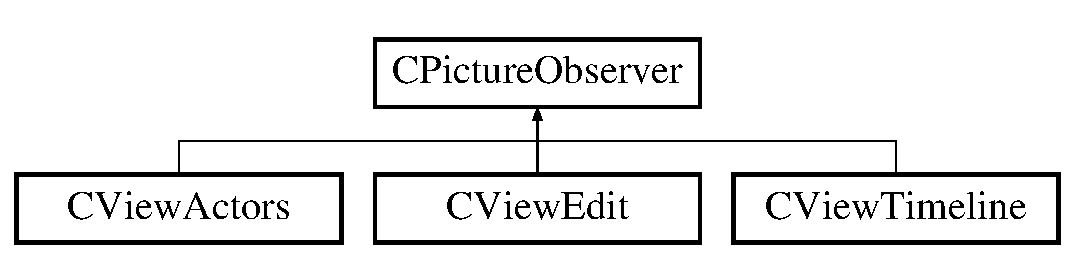
\includegraphics[height=2.000000cm]{class_c_picture_observer}
\end{center}
\end{figure}
\subsection*{Public Member Functions}
\begin{DoxyCompactItemize}
\item 
\hypertarget{class_c_picture_observer_a7c0cae97a7c165b98a00aeb2892cd6e7}{\hyperlink{class_c_picture_observer_a7c0cae97a7c165b98a00aeb2892cd6e7}{C\+Picture\+Observer} (const \hyperlink{class_c_picture_observer}{C\+Picture\+Observer} \&)=delete}\label{class_c_picture_observer_a7c0cae97a7c165b98a00aeb2892cd6e7}

\begin{DoxyCompactList}\small\item\em Copy Constructor (Disabled) \end{DoxyCompactList}\item 
\hypertarget{class_c_picture_observer_a200c66fe9ab13e18e9559033165b1895}{\hyperlink{class_c_picture_observer}{C\+Picture\+Observer} \& \hyperlink{class_c_picture_observer_a200c66fe9ab13e18e9559033165b1895}{operator=} (const \hyperlink{class_c_picture_observer}{C\+Picture\+Observer} \&)=delete}\label{class_c_picture_observer_a200c66fe9ab13e18e9559033165b1895}

\begin{DoxyCompactList}\small\item\em Assignment Operator (Disabled) \end{DoxyCompactList}\item 
\hypertarget{class_c_picture_observer_a0dce27216a8cb8a2490f0efc83a5994a}{virtual void \hyperlink{class_c_picture_observer_a0dce27216a8cb8a2490f0efc83a5994a}{Update\+Observer} ()=0}\label{class_c_picture_observer_a0dce27216a8cb8a2490f0efc83a5994a}

\begin{DoxyCompactList}\small\item\em This function is called to update any observers. \end{DoxyCompactList}\item 
virtual \hyperlink{class_c_picture_observer_a86036f6ad66ae4bad3f204f61d234f46}{$\sim$\+C\+Picture\+Observer} ()
\begin{DoxyCompactList}\small\item\em D\+Estructor. \end{DoxyCompactList}\item 
std\+::shared\+\_\+ptr$<$ \hyperlink{class_c_picture}{C\+Picture} $>$ \hyperlink{class_c_picture_observer_ab7613c4badd101ace6a992b2eaaea153}{Get\+Picture} ()
\item 
void \hyperlink{class_c_picture_observer_a8f4bd1a0d4e3b14b511d572a6dadeb7e}{Set\+Picture} (std\+::shared\+\_\+ptr$<$ \hyperlink{class_c_picture}{C\+Picture} $>$ picture)
\end{DoxyCompactItemize}
\subsection*{Protected Member Functions}
\begin{DoxyCompactItemize}
\item 
\hyperlink{class_c_picture_observer_a99e9a1639d81fcdb816921231fd10b99}{C\+Picture\+Observer} ()
\end{DoxyCompactItemize}


\subsection{Detailed Description}
Observer base class for a picture.

This class implements the base class functionality for an observer in the observer pattern. 

\subsection{Constructor \& Destructor Documentation}
\hypertarget{class_c_picture_observer_a86036f6ad66ae4bad3f204f61d234f46}{\index{C\+Picture\+Observer@{C\+Picture\+Observer}!````~C\+Picture\+Observer@{$\sim$\+C\+Picture\+Observer}}
\index{````~C\+Picture\+Observer@{$\sim$\+C\+Picture\+Observer}!C\+Picture\+Observer@{C\+Picture\+Observer}}
\subsubsection[{$\sim$\+C\+Picture\+Observer}]{\setlength{\rightskip}{0pt plus 5cm}C\+Picture\+Observer\+::$\sim$\+C\+Picture\+Observer (
\begin{DoxyParamCaption}
{}
\end{DoxyParamCaption}
)\hspace{0.3cm}{\ttfamily [virtual]}}}\label{class_c_picture_observer_a86036f6ad66ae4bad3f204f61d234f46}


D\+Estructor. 

Destructor \hypertarget{class_c_picture_observer_a99e9a1639d81fcdb816921231fd10b99}{\index{C\+Picture\+Observer@{C\+Picture\+Observer}!C\+Picture\+Observer@{C\+Picture\+Observer}}
\index{C\+Picture\+Observer@{C\+Picture\+Observer}!C\+Picture\+Observer@{C\+Picture\+Observer}}
\subsubsection[{C\+Picture\+Observer}]{\setlength{\rightskip}{0pt plus 5cm}C\+Picture\+Observer\+::\+C\+Picture\+Observer (
\begin{DoxyParamCaption}
{}
\end{DoxyParamCaption}
)\hspace{0.3cm}{\ttfamily [protected]}}}\label{class_c_picture_observer_a99e9a1639d81fcdb816921231fd10b99}
Constructor 

\subsection{Member Function Documentation}
\hypertarget{class_c_picture_observer_ab7613c4badd101ace6a992b2eaaea153}{\index{C\+Picture\+Observer@{C\+Picture\+Observer}!Get\+Picture@{Get\+Picture}}
\index{Get\+Picture@{Get\+Picture}!C\+Picture\+Observer@{C\+Picture\+Observer}}
\subsubsection[{Get\+Picture}]{\setlength{\rightskip}{0pt plus 5cm}std\+::shared\+\_\+ptr$<${\bf C\+Picture}$>$ C\+Picture\+Observer\+::\+Get\+Picture (
\begin{DoxyParamCaption}
{}
\end{DoxyParamCaption}
)\hspace{0.3cm}{\ttfamily [inline]}}}\label{class_c_picture_observer_ab7613c4badd101ace6a992b2eaaea153}
Get picture \begin{DoxyReturn}{Returns}
picture member vairable 
\end{DoxyReturn}
\hypertarget{class_c_picture_observer_a8f4bd1a0d4e3b14b511d572a6dadeb7e}{\index{C\+Picture\+Observer@{C\+Picture\+Observer}!Set\+Picture@{Set\+Picture}}
\index{Set\+Picture@{Set\+Picture}!C\+Picture\+Observer@{C\+Picture\+Observer}}
\subsubsection[{Set\+Picture}]{\setlength{\rightskip}{0pt plus 5cm}void C\+Picture\+Observer\+::\+Set\+Picture (
\begin{DoxyParamCaption}
\item[{std\+::shared\+\_\+ptr$<$ {\bf C\+Picture} $>$}]{picture}
\end{DoxyParamCaption}
)}}\label{class_c_picture_observer_a8f4bd1a0d4e3b14b511d572a6dadeb7e}
Set picture 
\begin{DoxyParams}{Parameters}
{\em picture} & member vairable\\
\hline
\end{DoxyParams}
Set the picture for this observer 
\begin{DoxyParams}{Parameters}
{\em picture} & The picture to set \\
\hline
\end{DoxyParams}


The documentation for this class was generated from the following files\+:\begin{DoxyCompactItemize}
\item 
\hyperlink{_picture_observer_8h}{Picture\+Observer.\+h}\item 
\hyperlink{_picture_observer_8cpp}{Picture\+Observer.\+cpp}\end{DoxyCompactItemize}

\hypertarget{class_c_poly_drawable}{\section{C\+Poly\+Drawable Class Reference}
\label{class_c_poly_drawable}\index{C\+Poly\+Drawable@{C\+Poly\+Drawable}}
}


{\ttfamily \#include $<$Poly\+Drawable.\+h$>$}

Inheritance diagram for C\+Poly\+Drawable\+:\begin{figure}[H]
\begin{center}
\leavevmode
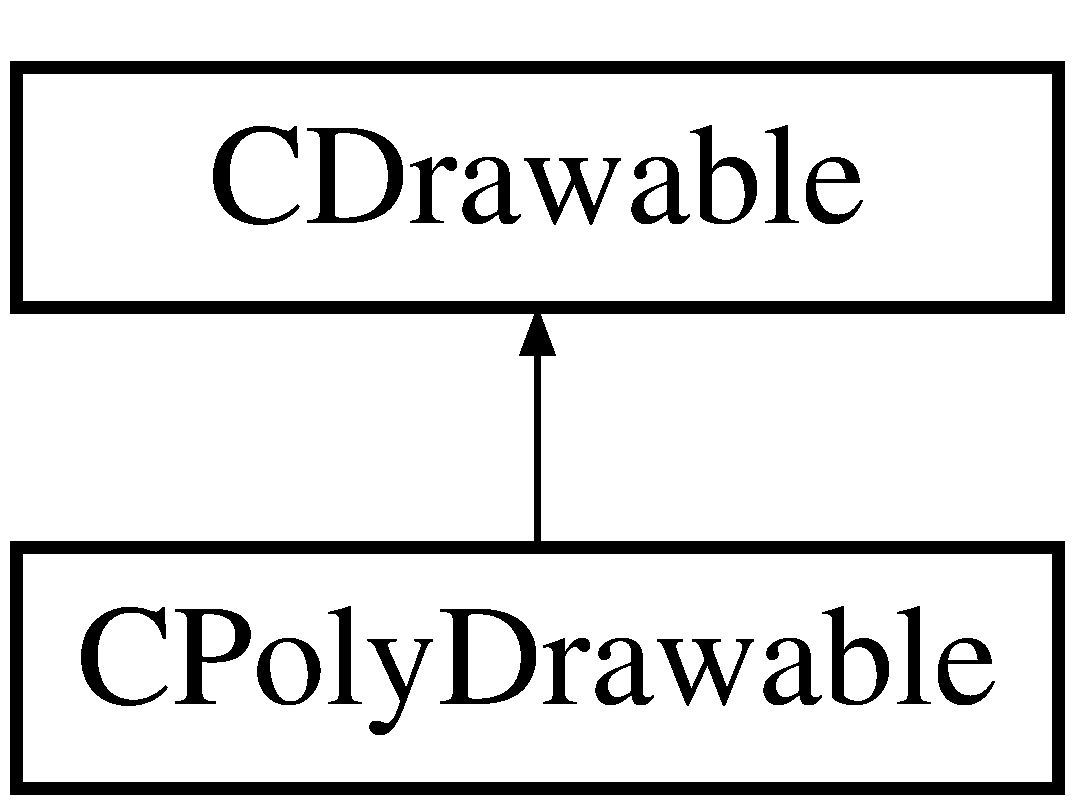
\includegraphics[height=2.000000cm]{class_c_poly_drawable}
\end{center}
\end{figure}
\subsection*{Public Member Functions}
\begin{DoxyCompactItemize}
\item 
\hypertarget{class_c_poly_drawable_ae4265afa898200aa70a943cdea3f8123}{\hyperlink{class_c_poly_drawable_ae4265afa898200aa70a943cdea3f8123}{C\+Poly\+Drawable} ()=delete}\label{class_c_poly_drawable_ae4265afa898200aa70a943cdea3f8123}

\begin{DoxyCompactList}\small\item\em Default constructor disabled. \end{DoxyCompactList}\item 
\hypertarget{class_c_poly_drawable_abfdd10484ab2cb6ea99c01849cad4082}{\hyperlink{class_c_poly_drawable_abfdd10484ab2cb6ea99c01849cad4082}{C\+Poly\+Drawable} (const \hyperlink{class_c_poly_drawable}{C\+Poly\+Drawable} \&)=delete}\label{class_c_poly_drawable_abfdd10484ab2cb6ea99c01849cad4082}

\begin{DoxyCompactList}\small\item\em Copy constructor disabled. \end{DoxyCompactList}\item 
\hypertarget{class_c_poly_drawable_a86a6c65081b7feb556e5563b36a6ac8a}{void \hyperlink{class_c_poly_drawable_a86a6c65081b7feb556e5563b36a6ac8a}{operator=} (const \hyperlink{class_c_poly_drawable}{C\+Poly\+Drawable} \&)=delete}\label{class_c_poly_drawable_a86a6c65081b7feb556e5563b36a6ac8a}

\begin{DoxyCompactList}\small\item\em Assignment operator disabled. \end{DoxyCompactList}\item 
\hyperlink{class_c_poly_drawable_a0afc2421a1a15fa7065423ccbe6d6ecc}{C\+Poly\+Drawable} (const std\+::wstring \&name)
\item 
Gdiplus\+::\+Color \hyperlink{class_c_poly_drawable_ab14b6cfd0e8c3ae025daa43465a1811f}{Get\+Color} ()
\begin{DoxyCompactList}\small\item\em Get colors. \end{DoxyCompactList}\item 
void \hyperlink{class_c_poly_drawable_a9f53b3d0a6ee9aa6f34a0c44a5a2cd66}{Set\+Color} (Gdiplus\+::\+Color incolor)
\begin{DoxyCompactList}\small\item\em set colors \end{DoxyCompactList}\item 
void \hyperlink{class_c_poly_drawable_a500a475002f4be3cfe6ed865aea0a827}{Add\+Point} (Gdiplus\+::\+Point point)
\begin{DoxyCompactList}\small\item\em adds a point \end{DoxyCompactList}\item 
void \hyperlink{class_c_poly_drawable_a30d59469ee2db1cd0bf786ffff031bdf}{Draw} (Gdiplus\+::\+Graphics $\ast$graphics)
\begin{DoxyCompactList}\small\item\em draws \end{DoxyCompactList}\item 
bool \hyperlink{class_c_poly_drawable_af45e78d42d9eee657e0bedde0fe003e4}{Hit\+Test} (Gdiplus\+::\+Point pos)
\end{DoxyCompactItemize}
\subsection*{Additional Inherited Members}


\subsection{Detailed Description}
A drawable based on polygon images.

This class has a list of points and draws a polygon drawable based on those points. 

\subsection{Constructor \& Destructor Documentation}
\hypertarget{class_c_poly_drawable_a0afc2421a1a15fa7065423ccbe6d6ecc}{\index{C\+Poly\+Drawable@{C\+Poly\+Drawable}!C\+Poly\+Drawable@{C\+Poly\+Drawable}}
\index{C\+Poly\+Drawable@{C\+Poly\+Drawable}!C\+Poly\+Drawable@{C\+Poly\+Drawable}}
\subsubsection[{C\+Poly\+Drawable}]{\setlength{\rightskip}{0pt plus 5cm}C\+Poly\+Drawable\+::\+C\+Poly\+Drawable (
\begin{DoxyParamCaption}
\item[{const std\+::wstring \&}]{name}
\end{DoxyParamCaption}
)}}\label{class_c_poly_drawable_a0afc2421a1a15fa7065423ccbe6d6ecc}
Constructor 
\begin{DoxyParams}{Parameters}
{\em name} & The drawable name \\
\hline
\end{DoxyParams}


\subsection{Member Function Documentation}
\hypertarget{class_c_poly_drawable_a500a475002f4be3cfe6ed865aea0a827}{\index{C\+Poly\+Drawable@{C\+Poly\+Drawable}!Add\+Point@{Add\+Point}}
\index{Add\+Point@{Add\+Point}!C\+Poly\+Drawable@{C\+Poly\+Drawable}}
\subsubsection[{Add\+Point}]{\setlength{\rightskip}{0pt plus 5cm}void C\+Poly\+Drawable\+::\+Add\+Point (
\begin{DoxyParamCaption}
\item[{Gdiplus\+::\+Point}]{point}
\end{DoxyParamCaption}
)\hspace{0.3cm}{\ttfamily [inline]}}}\label{class_c_poly_drawable_a500a475002f4be3cfe6ed865aea0a827}


adds a point 


\begin{DoxyParams}{Parameters}
{\em point} & to add \\
\hline
\end{DoxyParams}
\hypertarget{class_c_poly_drawable_a30d59469ee2db1cd0bf786ffff031bdf}{\index{C\+Poly\+Drawable@{C\+Poly\+Drawable}!Draw@{Draw}}
\index{Draw@{Draw}!C\+Poly\+Drawable@{C\+Poly\+Drawable}}
\subsubsection[{Draw}]{\setlength{\rightskip}{0pt plus 5cm}void C\+Poly\+Drawable\+::\+Draw (
\begin{DoxyParamCaption}
\item[{Gdiplus\+::\+Graphics $\ast$}]{graphics}
\end{DoxyParamCaption}
)\hspace{0.3cm}{\ttfamily [virtual]}}}\label{class_c_poly_drawable_a30d59469ee2db1cd0bf786ffff031bdf}


draws 


\begin{DoxyParams}{Parameters}
{\em graphics} & to draw\\
\hline
\end{DoxyParams}
Draw our polygon. 
\begin{DoxyParams}{Parameters}
{\em graphics} & The graphics context to draw on \\
\hline
\end{DoxyParams}


Implements \hyperlink{class_c_drawable_a9b6a9920a75d88d9ae321997495eaec7}{C\+Drawable}.

\hypertarget{class_c_poly_drawable_ab14b6cfd0e8c3ae025daa43465a1811f}{\index{C\+Poly\+Drawable@{C\+Poly\+Drawable}!Get\+Color@{Get\+Color}}
\index{Get\+Color@{Get\+Color}!C\+Poly\+Drawable@{C\+Poly\+Drawable}}
\subsubsection[{Get\+Color}]{\setlength{\rightskip}{0pt plus 5cm}Gdiplus\+::\+Color C\+Poly\+Drawable\+::\+Get\+Color (
\begin{DoxyParamCaption}
{}
\end{DoxyParamCaption}
)\hspace{0.3cm}{\ttfamily [inline]}}}\label{class_c_poly_drawable_ab14b6cfd0e8c3ae025daa43465a1811f}


Get colors. 

\begin{DoxyReturn}{Returns}
member var color 
\end{DoxyReturn}
\hypertarget{class_c_poly_drawable_af45e78d42d9eee657e0bedde0fe003e4}{\index{C\+Poly\+Drawable@{C\+Poly\+Drawable}!Hit\+Test@{Hit\+Test}}
\index{Hit\+Test@{Hit\+Test}!C\+Poly\+Drawable@{C\+Poly\+Drawable}}
\subsubsection[{Hit\+Test}]{\setlength{\rightskip}{0pt plus 5cm}bool C\+Poly\+Drawable\+::\+Hit\+Test (
\begin{DoxyParamCaption}
\item[{Gdiplus\+::\+Point}]{pos}
\end{DoxyParamCaption}
)\hspace{0.3cm}{\ttfamily [virtual]}}}\label{class_c_poly_drawable_af45e78d42d9eee657e0bedde0fe003e4}
hit test 
\begin{DoxyParams}{Parameters}
{\em pos} & position\\
\hline
\end{DoxyParams}
Test to see if we hit this object with a mouse click 
\begin{DoxyParams}{Parameters}
{\em pos} & Click position \\
\hline
\end{DoxyParams}
\begin{DoxyReturn}{Returns}
true it hit 
\end{DoxyReturn}


Implements \hyperlink{class_c_drawable_af715bc2e79788b2a44a74ad70b181544}{C\+Drawable}.

\hypertarget{class_c_poly_drawable_a9f53b3d0a6ee9aa6f34a0c44a5a2cd66}{\index{C\+Poly\+Drawable@{C\+Poly\+Drawable}!Set\+Color@{Set\+Color}}
\index{Set\+Color@{Set\+Color}!C\+Poly\+Drawable@{C\+Poly\+Drawable}}
\subsubsection[{Set\+Color}]{\setlength{\rightskip}{0pt plus 5cm}void C\+Poly\+Drawable\+::\+Set\+Color (
\begin{DoxyParamCaption}
\item[{Gdiplus\+::\+Color}]{incolor}
\end{DoxyParamCaption}
)\hspace{0.3cm}{\ttfamily [inline]}}}\label{class_c_poly_drawable_a9f53b3d0a6ee9aa6f34a0c44a5a2cd66}


set colors 


\begin{DoxyParams}{Parameters}
{\em incolor} & sets member var color \\
\hline
\end{DoxyParams}


The documentation for this class was generated from the following files\+:\begin{DoxyCompactItemize}
\item 
\hyperlink{_poly_drawable_8h}{Poly\+Drawable.\+h}\item 
Poly\+Drawable.\+cpp\end{DoxyCompactItemize}

\hypertarget{class_c_quinn_factory}{\section{C\+Quinn\+Factory Class Reference}
\label{class_c_quinn_factory}\index{C\+Quinn\+Factory@{C\+Quinn\+Factory}}
}


{\ttfamily \#include $<$Quinn\+Factory.\+h$>$}

Inheritance diagram for C\+Quinn\+Factory\+:\begin{figure}[H]
\begin{center}
\leavevmode
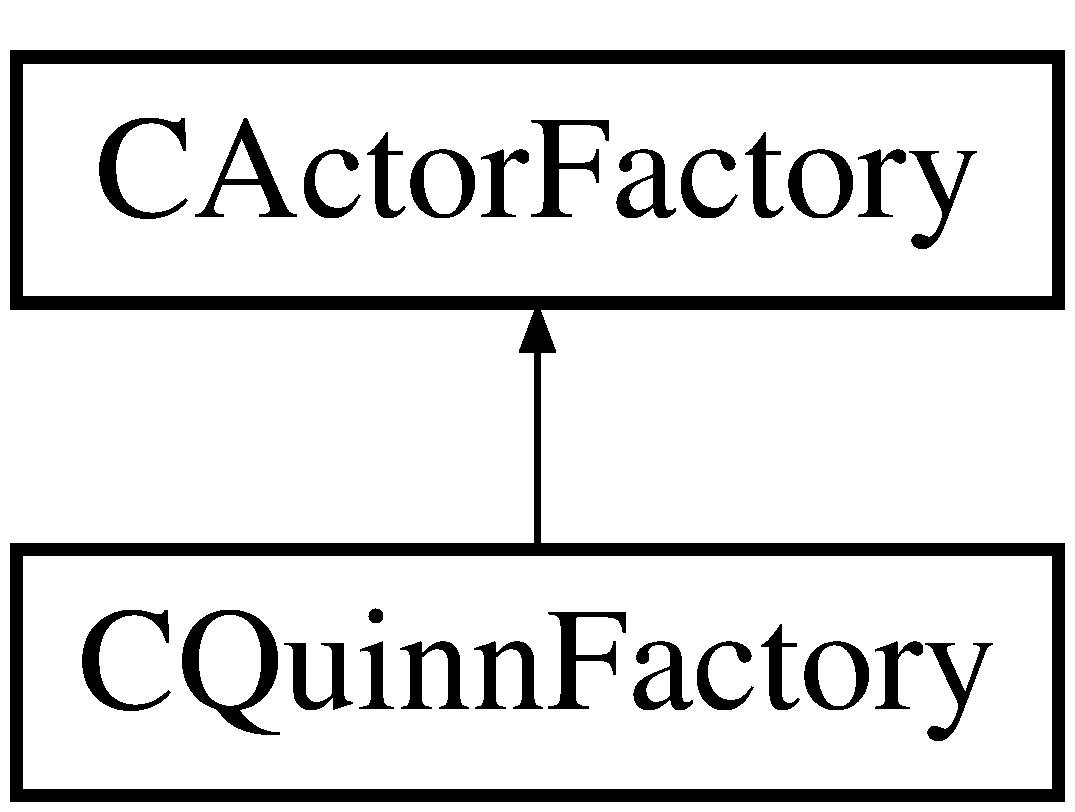
\includegraphics[height=2.000000cm]{class_c_quinn_factory}
\end{center}
\end{figure}
\subsection*{Public Member Functions}
\begin{DoxyCompactItemize}
\item 
std\+::shared\+\_\+ptr$<$ \hyperlink{class_c_actor}{C\+Actor} $>$ \hyperlink{class_c_quinn_factory_a94cca4731a6cc6e8790235618a468ff9}{Create} ()
\end{DoxyCompactItemize}


\subsection{Detailed Description}
Factory class that builds the Quinn character 

\subsection{Member Function Documentation}
\hypertarget{class_c_quinn_factory_a94cca4731a6cc6e8790235618a468ff9}{\index{C\+Quinn\+Factory@{C\+Quinn\+Factory}!Create@{Create}}
\index{Create@{Create}!C\+Quinn\+Factory@{C\+Quinn\+Factory}}
\subsubsection[{Create}]{\setlength{\rightskip}{0pt plus 5cm}std\+::shared\+\_\+ptr$<$ {\bf C\+Actor} $>$ C\+Quinn\+Factory\+::\+Create (
\begin{DoxyParamCaption}
{}
\end{DoxyParamCaption}
)}}\label{class_c_quinn_factory_a94cca4731a6cc6e8790235618a468ff9}
This is a concrete factory method that creates our Harold actor. \begin{DoxyReturn}{Returns}
Pointer to an actor object. 
\end{DoxyReturn}


The documentation for this class was generated from the following files\+:\begin{DoxyCompactItemize}
\item 
\hyperlink{_quinn_factory_8h}{Quinn\+Factory.\+h}\item 
\hyperlink{_quinn_factory_8cpp}{Quinn\+Factory.\+cpp}\end{DoxyCompactItemize}

\hypertarget{class_c_view_actors}{\section{C\+View\+Actors Class Reference}
\label{class_c_view_actors}\index{C\+View\+Actors@{C\+View\+Actors}}
}


{\ttfamily \#include $<$View\+Actors.\+h$>$}

Inheritance diagram for C\+View\+Actors\+:\begin{figure}[H]
\begin{center}
\leavevmode
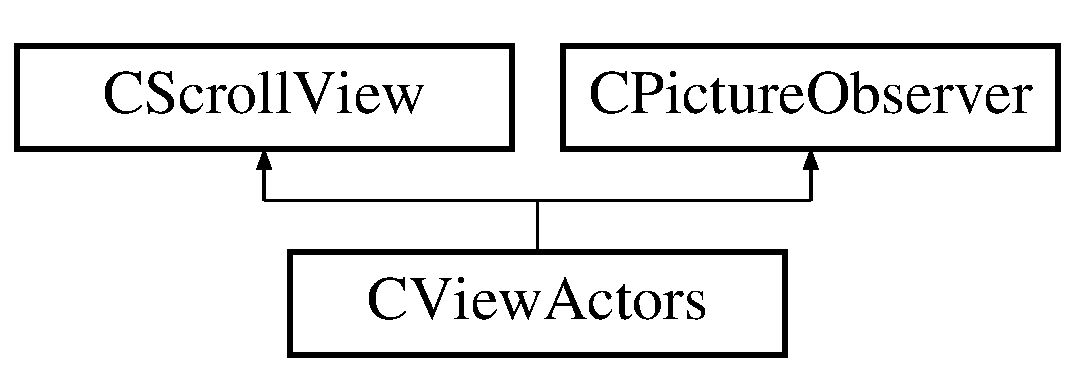
\includegraphics[height=2.000000cm]{class_c_view_actors}
\end{center}
\end{figure}
\subsection*{Public Member Functions}
\begin{DoxyCompactItemize}
\item 
afx\+\_\+msg B\+O\+O\+L \hyperlink{class_c_view_actors_a561f4be212bd5df4a667c2cb0b23e472}{On\+Erase\+Bkgnd} (C\+D\+C $\ast$p\+D\+C)
\item 
void \hyperlink{class_c_view_actors_a6f68ae9e71f6a195502464bf34b3e724}{Set\+Main\+Frame} (\hyperlink{class_c_main_frame}{C\+Main\+Frame} $\ast$main\+Frame)
\end{DoxyCompactItemize}
\subsection*{Static Public Attributes}
\begin{DoxyCompactItemize}
\item 
\hypertarget{class_c_view_actors_a8bb27cbe8ae099abbed012adca884f1f}{static const int \hyperlink{class_c_view_actors_a8bb27cbe8ae099abbed012adca884f1f}{Width} = 150}\label{class_c_view_actors_a8bb27cbe8ae099abbed012adca884f1f}

\begin{DoxyCompactList}\small\item\em Width we want for this window. \end{DoxyCompactList}\end{DoxyCompactItemize}
\subsection*{Protected Member Functions}
\begin{DoxyCompactItemize}
\item 
\hyperlink{class_c_view_actors_aeff00d958ecea52760ec07c0420c4e28}{C\+View\+Actors} ()
\begin{DoxyCompactList}\small\item\em $\ast$/ \end{DoxyCompactList}\item 
virtual \hyperlink{class_c_view_actors_a6e1aa1c82708dd805ac90c21b6d521e0}{$\sim$\+C\+View\+Actors} ()
\item 
virtual void \hyperlink{class_c_view_actors_a5014f8c616850b8e874dee895b2ba698}{Update\+Observer} () override
\item 
virtual void \hyperlink{class_c_view_actors_aa68465c2f13e487426508832a6355503}{On\+Draw} (C\+D\+C $\ast$p\+D\+C)
\item 
virtual void \hyperlink{class_c_view_actors_aaf83b3647a42330c01be9067a6235d33}{On\+Initial\+Update} ()
\end{DoxyCompactItemize}


\subsection{Detailed Description}
Class that provides a view windows for actors. 

\subsection{Constructor \& Destructor Documentation}
\hypertarget{class_c_view_actors_aeff00d958ecea52760ec07c0420c4e28}{\index{C\+View\+Actors@{C\+View\+Actors}!C\+View\+Actors@{C\+View\+Actors}}
\index{C\+View\+Actors@{C\+View\+Actors}!C\+View\+Actors@{C\+View\+Actors}}
\subsubsection[{C\+View\+Actors}]{\setlength{\rightskip}{0pt plus 5cm}C\+View\+Actors\+::\+C\+View\+Actors (
\begin{DoxyParamCaption}
{}
\end{DoxyParamCaption}
)\hspace{0.3cm}{\ttfamily [protected]}}}\label{class_c_view_actors_aeff00d958ecea52760ec07c0420c4e28}


$\ast$/ 

Constructor \hypertarget{class_c_view_actors_a6e1aa1c82708dd805ac90c21b6d521e0}{\index{C\+View\+Actors@{C\+View\+Actors}!````~C\+View\+Actors@{$\sim$\+C\+View\+Actors}}
\index{````~C\+View\+Actors@{$\sim$\+C\+View\+Actors}!C\+View\+Actors@{C\+View\+Actors}}
\subsubsection[{$\sim$\+C\+View\+Actors}]{\setlength{\rightskip}{0pt plus 5cm}C\+View\+Actors\+::$\sim$\+C\+View\+Actors (
\begin{DoxyParamCaption}
{}
\end{DoxyParamCaption}
)\hspace{0.3cm}{\ttfamily [protected]}, {\ttfamily [virtual]}}}\label{class_c_view_actors_a6e1aa1c82708dd805ac90c21b6d521e0}
Destructor 

\subsection{Member Function Documentation}
\hypertarget{class_c_view_actors_aa68465c2f13e487426508832a6355503}{\index{C\+View\+Actors@{C\+View\+Actors}!On\+Draw@{On\+Draw}}
\index{On\+Draw@{On\+Draw}!C\+View\+Actors@{C\+View\+Actors}}
\subsubsection[{On\+Draw}]{\setlength{\rightskip}{0pt plus 5cm}void C\+View\+Actors\+::\+On\+Draw (
\begin{DoxyParamCaption}
\item[{C\+D\+C $\ast$}]{p\+D\+C}
\end{DoxyParamCaption}
)\hspace{0.3cm}{\ttfamily [protected]}, {\ttfamily [virtual]}}}\label{class_c_view_actors_aa68465c2f13e487426508832a6355503}
Draw this window 
\begin{DoxyParams}{Parameters}
{\em p\+D\+C} & Device context \\
\hline
\end{DoxyParams}
\hypertarget{class_c_view_actors_a561f4be212bd5df4a667c2cb0b23e472}{\index{C\+View\+Actors@{C\+View\+Actors}!On\+Erase\+Bkgnd@{On\+Erase\+Bkgnd}}
\index{On\+Erase\+Bkgnd@{On\+Erase\+Bkgnd}!C\+View\+Actors@{C\+View\+Actors}}
\subsubsection[{On\+Erase\+Bkgnd}]{\setlength{\rightskip}{0pt plus 5cm}B\+O\+O\+L C\+View\+Actors\+::\+On\+Erase\+Bkgnd (
\begin{DoxyParamCaption}
\item[{C\+D\+C $\ast$}]{p\+D\+C}
\end{DoxyParamCaption}
)}}\label{class_c_view_actors_a561f4be212bd5df4a667c2cb0b23e472}
Erase the background

This is disabled to eliminate flicker 
\begin{DoxyParams}{Parameters}
{\em p\+D\+C} & Device context \\
\hline
\end{DoxyParams}
\begin{DoxyReturn}{Returns}
F\+A\+L\+S\+E 
\end{DoxyReturn}
\hypertarget{class_c_view_actors_aaf83b3647a42330c01be9067a6235d33}{\index{C\+View\+Actors@{C\+View\+Actors}!On\+Initial\+Update@{On\+Initial\+Update}}
\index{On\+Initial\+Update@{On\+Initial\+Update}!C\+View\+Actors@{C\+View\+Actors}}
\subsubsection[{On\+Initial\+Update}]{\setlength{\rightskip}{0pt plus 5cm}void C\+View\+Actors\+::\+On\+Initial\+Update (
\begin{DoxyParamCaption}
{}
\end{DoxyParamCaption}
)\hspace{0.3cm}{\ttfamily [protected]}, {\ttfamily [virtual]}}}\label{class_c_view_actors_aaf83b3647a42330c01be9067a6235d33}
Handle the initial update for this window \hypertarget{class_c_view_actors_a6f68ae9e71f6a195502464bf34b3e724}{\index{C\+View\+Actors@{C\+View\+Actors}!Set\+Main\+Frame@{Set\+Main\+Frame}}
\index{Set\+Main\+Frame@{Set\+Main\+Frame}!C\+View\+Actors@{C\+View\+Actors}}
\subsubsection[{Set\+Main\+Frame}]{\setlength{\rightskip}{0pt plus 5cm}void C\+View\+Actors\+::\+Set\+Main\+Frame (
\begin{DoxyParamCaption}
\item[{{\bf C\+Main\+Frame} $\ast$}]{main\+Frame}
\end{DoxyParamCaption}
)\hspace{0.3cm}{\ttfamily [inline]}}}\label{class_c_view_actors_a6f68ae9e71f6a195502464bf34b3e724}
Set the main\+Frame pointer 
\begin{DoxyParams}{Parameters}
{\em main\+Frame} & Pointer to the \hyperlink{class_c_main_frame}{C\+Main\+Frame} window \\
\hline
\end{DoxyParams}
\hypertarget{class_c_view_actors_a5014f8c616850b8e874dee895b2ba698}{\index{C\+View\+Actors@{C\+View\+Actors}!Update\+Observer@{Update\+Observer}}
\index{Update\+Observer@{Update\+Observer}!C\+View\+Actors@{C\+View\+Actors}}
\subsubsection[{Update\+Observer}]{\setlength{\rightskip}{0pt plus 5cm}void C\+View\+Actors\+::\+Update\+Observer (
\begin{DoxyParamCaption}
{}
\end{DoxyParamCaption}
)\hspace{0.3cm}{\ttfamily [override]}, {\ttfamily [protected]}, {\ttfamily [virtual]}}}\label{class_c_view_actors_a5014f8c616850b8e874dee895b2ba698}
Force an update of this window when the picture changes. 

Implements \hyperlink{class_c_picture_observer_a0dce27216a8cb8a2490f0efc83a5994a}{C\+Picture\+Observer}.



The documentation for this class was generated from the following files\+:\begin{DoxyCompactItemize}
\item 
\hyperlink{_view_actors_8h}{View\+Actors.\+h}\item 
\hyperlink{_view_actors_8cpp}{View\+Actors.\+cpp}\end{DoxyCompactItemize}

\hypertarget{class_c_view_edit}{\section{C\+View\+Edit Class Reference}
\label{class_c_view_edit}\index{C\+View\+Edit@{C\+View\+Edit}}
}


{\ttfamily \#include $<$View\+Edit.\+h$>$}

Inheritance diagram for C\+View\+Edit\+:\begin{figure}[H]
\begin{center}
\leavevmode
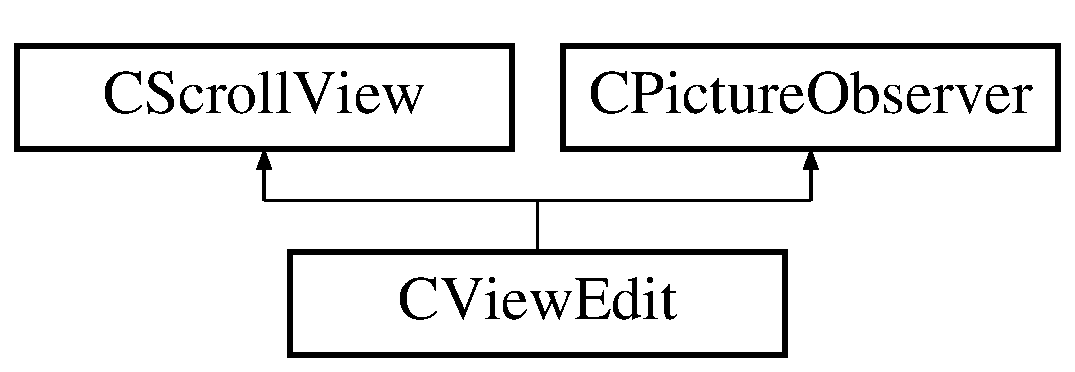
\includegraphics[height=2.000000cm]{class_c_view_edit}
\end{center}
\end{figure}
\subsection*{Public Member Functions}
\begin{DoxyCompactItemize}
\item 
\hyperlink{class_c_view_edit_a99fea37450207a1ffe8cf6b46ec2a11f}{C\+View\+Edit} ()
\item 
virtual \hyperlink{class_c_view_edit_a968f16ef61489033c80ebe504017db3a}{$\sim$\+C\+View\+Edit} ()
\item 
virtual void \hyperlink{class_c_view_edit_ac2b73f20fe10a4a98096facde6450e5a}{Update\+Observer} () override
\item 
afx\+\_\+msg B\+O\+O\+L \hyperlink{class_c_view_edit_a66446b22920245bb3b5c5735754d63cd}{On\+Erase\+Bkgnd} (C\+D\+C $\ast$p\+D\+C)
\item 
afx\+\_\+msg void \hyperlink{class_c_view_edit_a0e77d59dd1ed299c933f660d9ff0cf7e}{On\+L\+Button\+Down} (U\+I\+N\+T n\+Flags, C\+Point point)
\item 
afx\+\_\+msg void \hyperlink{class_c_view_edit_aba0b38ee4b51f9d98bc08ade92d9f051}{On\+Mouse\+Move} (U\+I\+N\+T n\+Flags, C\+Point point)
\item 
void \hyperlink{class_c_view_edit_a28bb793d43baba78e9b1c704b4f0e128}{Set\+Main\+Frame} (\hyperlink{class_c_main_frame}{C\+Main\+Frame} $\ast$main\+Frame)
\end{DoxyCompactItemize}
\subsection*{Protected Member Functions}
\begin{DoxyCompactItemize}
\item 
virtual void \hyperlink{class_c_view_edit_a8cf50c2cebab5aaecda5ae6f7437cf38}{On\+Draw} (C\+D\+C $\ast$p\+D\+C)
\item 
virtual void \hyperlink{class_c_view_edit_ac49ed2e9e35cd014c6539aaa4ac705f3}{On\+Initial\+Update} ()
\end{DoxyCompactItemize}


\subsection{Detailed Description}
View class the provides a window for editing our pixture 

\subsection{Constructor \& Destructor Documentation}
\hypertarget{class_c_view_edit_a99fea37450207a1ffe8cf6b46ec2a11f}{\index{C\+View\+Edit@{C\+View\+Edit}!C\+View\+Edit@{C\+View\+Edit}}
\index{C\+View\+Edit@{C\+View\+Edit}!C\+View\+Edit@{C\+View\+Edit}}
\subsubsection[{C\+View\+Edit}]{\setlength{\rightskip}{0pt plus 5cm}C\+View\+Edit\+::\+C\+View\+Edit (
\begin{DoxyParamCaption}
{}
\end{DoxyParamCaption}
)}}\label{class_c_view_edit_a99fea37450207a1ffe8cf6b46ec2a11f}
Constructor \hypertarget{class_c_view_edit_a968f16ef61489033c80ebe504017db3a}{\index{C\+View\+Edit@{C\+View\+Edit}!````~C\+View\+Edit@{$\sim$\+C\+View\+Edit}}
\index{````~C\+View\+Edit@{$\sim$\+C\+View\+Edit}!C\+View\+Edit@{C\+View\+Edit}}
\subsubsection[{$\sim$\+C\+View\+Edit}]{\setlength{\rightskip}{0pt plus 5cm}C\+View\+Edit\+::$\sim$\+C\+View\+Edit (
\begin{DoxyParamCaption}
{}
\end{DoxyParamCaption}
)\hspace{0.3cm}{\ttfamily [virtual]}}}\label{class_c_view_edit_a968f16ef61489033c80ebe504017db3a}
Destructor 

\subsection{Member Function Documentation}
\hypertarget{class_c_view_edit_a8cf50c2cebab5aaecda5ae6f7437cf38}{\index{C\+View\+Edit@{C\+View\+Edit}!On\+Draw@{On\+Draw}}
\index{On\+Draw@{On\+Draw}!C\+View\+Edit@{C\+View\+Edit}}
\subsubsection[{On\+Draw}]{\setlength{\rightskip}{0pt plus 5cm}void C\+View\+Edit\+::\+On\+Draw (
\begin{DoxyParamCaption}
\item[{C\+D\+C $\ast$}]{p\+D\+C}
\end{DoxyParamCaption}
)\hspace{0.3cm}{\ttfamily [protected]}, {\ttfamily [virtual]}}}\label{class_c_view_edit_a8cf50c2cebab5aaecda5ae6f7437cf38}
Drawing of the window 
\begin{DoxyParams}{Parameters}
{\em p\+D\+C} & the device context to draw on \\
\hline
\end{DoxyParams}
\hypertarget{class_c_view_edit_a66446b22920245bb3b5c5735754d63cd}{\index{C\+View\+Edit@{C\+View\+Edit}!On\+Erase\+Bkgnd@{On\+Erase\+Bkgnd}}
\index{On\+Erase\+Bkgnd@{On\+Erase\+Bkgnd}!C\+View\+Edit@{C\+View\+Edit}}
\subsubsection[{On\+Erase\+Bkgnd}]{\setlength{\rightskip}{0pt plus 5cm}B\+O\+O\+L C\+View\+Edit\+::\+On\+Erase\+Bkgnd (
\begin{DoxyParamCaption}
\item[{C\+D\+C $\ast$}]{p\+D\+C}
\end{DoxyParamCaption}
)}}\label{class_c_view_edit_a66446b22920245bb3b5c5735754d63cd}
Erase the background

This is disabled to eliminate flicker 
\begin{DoxyParams}{Parameters}
{\em p\+D\+C} & Device context \\
\hline
\end{DoxyParams}
\begin{DoxyReturn}{Returns}
F\+A\+L\+S\+E 
\end{DoxyReturn}
\hypertarget{class_c_view_edit_ac49ed2e9e35cd014c6539aaa4ac705f3}{\index{C\+View\+Edit@{C\+View\+Edit}!On\+Initial\+Update@{On\+Initial\+Update}}
\index{On\+Initial\+Update@{On\+Initial\+Update}!C\+View\+Edit@{C\+View\+Edit}}
\subsubsection[{On\+Initial\+Update}]{\setlength{\rightskip}{0pt plus 5cm}void C\+View\+Edit\+::\+On\+Initial\+Update (
\begin{DoxyParamCaption}
{}
\end{DoxyParamCaption}
)\hspace{0.3cm}{\ttfamily [protected]}, {\ttfamily [virtual]}}}\label{class_c_view_edit_ac49ed2e9e35cd014c6539aaa4ac705f3}
Handle uial update of the window \hypertarget{class_c_view_edit_a0e77d59dd1ed299c933f660d9ff0cf7e}{\index{C\+View\+Edit@{C\+View\+Edit}!On\+L\+Button\+Down@{On\+L\+Button\+Down}}
\index{On\+L\+Button\+Down@{On\+L\+Button\+Down}!C\+View\+Edit@{C\+View\+Edit}}
\subsubsection[{On\+L\+Button\+Down}]{\setlength{\rightskip}{0pt plus 5cm}void C\+View\+Edit\+::\+On\+L\+Button\+Down (
\begin{DoxyParamCaption}
\item[{U\+I\+N\+T}]{n\+Flags, }
\item[{C\+Point}]{point}
\end{DoxyParamCaption}
)}}\label{class_c_view_edit_a0e77d59dd1ed299c933f660d9ff0cf7e}
Handle a left button click 
\begin{DoxyParams}{Parameters}
{\em n\+Flags} & Flags that indicate status of the mouse buttons \\
\hline
{\em point} & The x,y location for the mouse click \\
\hline
\end{DoxyParams}
\hypertarget{class_c_view_edit_aba0b38ee4b51f9d98bc08ade92d9f051}{\index{C\+View\+Edit@{C\+View\+Edit}!On\+Mouse\+Move@{On\+Mouse\+Move}}
\index{On\+Mouse\+Move@{On\+Mouse\+Move}!C\+View\+Edit@{C\+View\+Edit}}
\subsubsection[{On\+Mouse\+Move}]{\setlength{\rightskip}{0pt plus 5cm}void C\+View\+Edit\+::\+On\+Mouse\+Move (
\begin{DoxyParamCaption}
\item[{U\+I\+N\+T}]{n\+Flags, }
\item[{C\+Point}]{point}
\end{DoxyParamCaption}
)}}\label{class_c_view_edit_aba0b38ee4b51f9d98bc08ade92d9f051}
Handle mouse movement 
\begin{DoxyParams}{Parameters}
{\em n\+Flags} & Flags that indicate status of the mouse buttons \\
\hline
{\em point} & The x,y location for the mouse \\
\hline
\end{DoxyParams}
\hypertarget{class_c_view_edit_a28bb793d43baba78e9b1c704b4f0e128}{\index{C\+View\+Edit@{C\+View\+Edit}!Set\+Main\+Frame@{Set\+Main\+Frame}}
\index{Set\+Main\+Frame@{Set\+Main\+Frame}!C\+View\+Edit@{C\+View\+Edit}}
\subsubsection[{Set\+Main\+Frame}]{\setlength{\rightskip}{0pt plus 5cm}void C\+View\+Edit\+::\+Set\+Main\+Frame (
\begin{DoxyParamCaption}
\item[{{\bf C\+Main\+Frame} $\ast$}]{main\+Frame}
\end{DoxyParamCaption}
)\hspace{0.3cm}{\ttfamily [inline]}}}\label{class_c_view_edit_a28bb793d43baba78e9b1c704b4f0e128}
Set the main\+Frame pointer 
\begin{DoxyParams}{Parameters}
{\em main\+Frame} & Pointer to the \hyperlink{class_c_main_frame}{C\+Main\+Frame} window \\
\hline
\end{DoxyParams}
\hypertarget{class_c_view_edit_ac2b73f20fe10a4a98096facde6450e5a}{\index{C\+View\+Edit@{C\+View\+Edit}!Update\+Observer@{Update\+Observer}}
\index{Update\+Observer@{Update\+Observer}!C\+View\+Edit@{C\+View\+Edit}}
\subsubsection[{Update\+Observer}]{\setlength{\rightskip}{0pt plus 5cm}void C\+View\+Edit\+::\+Update\+Observer (
\begin{DoxyParamCaption}
{}
\end{DoxyParamCaption}
)\hspace{0.3cm}{\ttfamily [override]}, {\ttfamily [virtual]}}}\label{class_c_view_edit_ac2b73f20fe10a4a98096facde6450e5a}
Force an update of this window when the picture changes. 

Implements \hyperlink{class_c_picture_observer_a0dce27216a8cb8a2490f0efc83a5994a}{C\+Picture\+Observer}.



The documentation for this class was generated from the following files\+:\begin{DoxyCompactItemize}
\item 
\hyperlink{_view_edit_8h}{View\+Edit.\+h}\item 
\hyperlink{_view_edit_8cpp}{View\+Edit.\+cpp}\end{DoxyCompactItemize}

\hypertarget{class_c_view_timeline}{\section{C\+View\+Timeline Class Reference}
\label{class_c_view_timeline}\index{C\+View\+Timeline@{C\+View\+Timeline}}
}


{\ttfamily \#include $<$View\+Timeline.\+h$>$}

Inheritance diagram for C\+View\+Timeline\+:\begin{figure}[H]
\begin{center}
\leavevmode
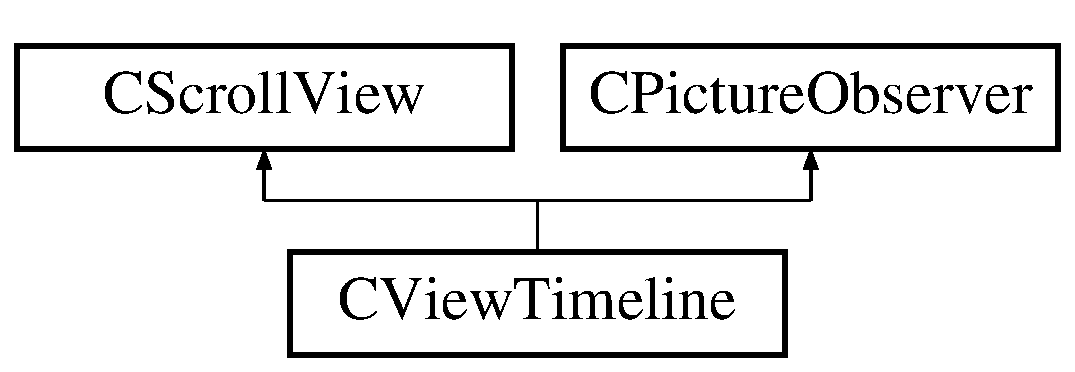
\includegraphics[height=2.000000cm]{class_c_view_timeline}
\end{center}
\end{figure}
\subsection*{Public Member Functions}
\begin{DoxyCompactItemize}
\item 
virtual void \hyperlink{class_c_view_timeline_a21388abd4726fd3dbe02b6e2ea313369}{Update\+Observer} () override
\item 
afx\+\_\+msg B\+O\+O\+L \hyperlink{class_c_view_timeline_a8328ae76e5f95d36b3ab7e8bbd8ef72f}{On\+Erase\+Bkgnd} (C\+D\+C $\ast$p\+D\+C)
\item 
afx\+\_\+msg void \hyperlink{class_c_view_timeline_acb22f2662a21152e607d17dbc293351c}{On\+Edit\+Setkeyframe} ()
\item 
afx\+\_\+msg void \hyperlink{class_c_view_timeline_ab3eccb4a5bcd5ffa60442359b86e0597}{On\+Edit\+Deletekeyframe} ()
\item 
void \hyperlink{class_c_view_timeline_aba069993dd75712f340999345e791327}{Set\+Main\+Frame} (\hyperlink{class_c_main_frame}{C\+Main\+Frame} $\ast$main\+Frame)
\end{DoxyCompactItemize}
\subsection*{Static Public Attributes}
\begin{DoxyCompactItemize}
\item 
\hypertarget{class_c_view_timeline_a6634479092090825e8c392902cf6c685}{static const int \hyperlink{class_c_view_timeline_a6634479092090825e8c392902cf6c685}{Height} = 90}\label{class_c_view_timeline_a6634479092090825e8c392902cf6c685}

\begin{DoxyCompactList}\small\item\em Height to make this window. \end{DoxyCompactList}\end{DoxyCompactItemize}
\subsection*{Protected Member Functions}
\begin{DoxyCompactItemize}
\item 
\hyperlink{class_c_view_timeline_aee8b6ebfaa9e299c65d6be0fc27b79f1}{C\+View\+Timeline} ()
\item 
virtual \hyperlink{class_c_view_timeline_afec58a7cb0dfafd6c64c19e9e8a57842}{$\sim$\+C\+View\+Timeline} ()
\item 
virtual void \hyperlink{class_c_view_timeline_a32f2ff1b162abc49f841e5dd6ddcb7df}{On\+Draw} (C\+D\+C $\ast$p\+D\+C)
\item 
virtual void \hyperlink{class_c_view_timeline_a7996d31301f034cf9fa59e3d846c5fb5}{On\+Initial\+Update} ()
\end{DoxyCompactItemize}


\subsection{Detailed Description}
View window for the animation timeline 

\subsection{Constructor \& Destructor Documentation}
\hypertarget{class_c_view_timeline_aee8b6ebfaa9e299c65d6be0fc27b79f1}{\index{C\+View\+Timeline@{C\+View\+Timeline}!C\+View\+Timeline@{C\+View\+Timeline}}
\index{C\+View\+Timeline@{C\+View\+Timeline}!C\+View\+Timeline@{C\+View\+Timeline}}
\subsubsection[{C\+View\+Timeline}]{\setlength{\rightskip}{0pt plus 5cm}C\+View\+Timeline\+::\+C\+View\+Timeline (
\begin{DoxyParamCaption}
{}
\end{DoxyParamCaption}
)\hspace{0.3cm}{\ttfamily [protected]}}}\label{class_c_view_timeline_aee8b6ebfaa9e299c65d6be0fc27b79f1}
Constructor \hypertarget{class_c_view_timeline_afec58a7cb0dfafd6c64c19e9e8a57842}{\index{C\+View\+Timeline@{C\+View\+Timeline}!````~C\+View\+Timeline@{$\sim$\+C\+View\+Timeline}}
\index{````~C\+View\+Timeline@{$\sim$\+C\+View\+Timeline}!C\+View\+Timeline@{C\+View\+Timeline}}
\subsubsection[{$\sim$\+C\+View\+Timeline}]{\setlength{\rightskip}{0pt plus 5cm}C\+View\+Timeline\+::$\sim$\+C\+View\+Timeline (
\begin{DoxyParamCaption}
{}
\end{DoxyParamCaption}
)\hspace{0.3cm}{\ttfamily [protected]}, {\ttfamily [virtual]}}}\label{class_c_view_timeline_afec58a7cb0dfafd6c64c19e9e8a57842}
Destructor 

\subsection{Member Function Documentation}
\hypertarget{class_c_view_timeline_a32f2ff1b162abc49f841e5dd6ddcb7df}{\index{C\+View\+Timeline@{C\+View\+Timeline}!On\+Draw@{On\+Draw}}
\index{On\+Draw@{On\+Draw}!C\+View\+Timeline@{C\+View\+Timeline}}
\subsubsection[{On\+Draw}]{\setlength{\rightskip}{0pt plus 5cm}void C\+View\+Timeline\+::\+On\+Draw (
\begin{DoxyParamCaption}
\item[{C\+D\+C $\ast$}]{p\+D\+C}
\end{DoxyParamCaption}
)\hspace{0.3cm}{\ttfamily [protected]}, {\ttfamily [virtual]}}}\label{class_c_view_timeline_a32f2ff1b162abc49f841e5dd6ddcb7df}
Draw this window 
\begin{DoxyParams}{Parameters}
{\em p\+D\+C} & Device context \\
\hline
\end{DoxyParams}
\hypertarget{class_c_view_timeline_ab3eccb4a5bcd5ffa60442359b86e0597}{\index{C\+View\+Timeline@{C\+View\+Timeline}!On\+Edit\+Deletekeyframe@{On\+Edit\+Deletekeyframe}}
\index{On\+Edit\+Deletekeyframe@{On\+Edit\+Deletekeyframe}!C\+View\+Timeline@{C\+View\+Timeline}}
\subsubsection[{On\+Edit\+Deletekeyframe}]{\setlength{\rightskip}{0pt plus 5cm}void C\+View\+Timeline\+::\+On\+Edit\+Deletekeyframe (
\begin{DoxyParamCaption}
{}
\end{DoxyParamCaption}
)}}\label{class_c_view_timeline_ab3eccb4a5bcd5ffa60442359b86e0597}
Handle the Edit$>$Delete Keyframe menu option \hypertarget{class_c_view_timeline_acb22f2662a21152e607d17dbc293351c}{\index{C\+View\+Timeline@{C\+View\+Timeline}!On\+Edit\+Setkeyframe@{On\+Edit\+Setkeyframe}}
\index{On\+Edit\+Setkeyframe@{On\+Edit\+Setkeyframe}!C\+View\+Timeline@{C\+View\+Timeline}}
\subsubsection[{On\+Edit\+Setkeyframe}]{\setlength{\rightskip}{0pt plus 5cm}void C\+View\+Timeline\+::\+On\+Edit\+Setkeyframe (
\begin{DoxyParamCaption}
{}
\end{DoxyParamCaption}
)}}\label{class_c_view_timeline_acb22f2662a21152e607d17dbc293351c}
Handle the Edit$>$Set Keyframe menu option \hypertarget{class_c_view_timeline_a8328ae76e5f95d36b3ab7e8bbd8ef72f}{\index{C\+View\+Timeline@{C\+View\+Timeline}!On\+Erase\+Bkgnd@{On\+Erase\+Bkgnd}}
\index{On\+Erase\+Bkgnd@{On\+Erase\+Bkgnd}!C\+View\+Timeline@{C\+View\+Timeline}}
\subsubsection[{On\+Erase\+Bkgnd}]{\setlength{\rightskip}{0pt plus 5cm}B\+O\+O\+L C\+View\+Timeline\+::\+On\+Erase\+Bkgnd (
\begin{DoxyParamCaption}
\item[{C\+D\+C $\ast$}]{p\+D\+C}
\end{DoxyParamCaption}
)}}\label{class_c_view_timeline_a8328ae76e5f95d36b3ab7e8bbd8ef72f}
Erase the background

This is disabled to eliminate flicker 
\begin{DoxyParams}{Parameters}
{\em p\+D\+C} & Device context \\
\hline
\end{DoxyParams}
\begin{DoxyReturn}{Returns}
F\+A\+L\+S\+E 
\end{DoxyReturn}
\hypertarget{class_c_view_timeline_a7996d31301f034cf9fa59e3d846c5fb5}{\index{C\+View\+Timeline@{C\+View\+Timeline}!On\+Initial\+Update@{On\+Initial\+Update}}
\index{On\+Initial\+Update@{On\+Initial\+Update}!C\+View\+Timeline@{C\+View\+Timeline}}
\subsubsection[{On\+Initial\+Update}]{\setlength{\rightskip}{0pt plus 5cm}void C\+View\+Timeline\+::\+On\+Initial\+Update (
\begin{DoxyParamCaption}
{}
\end{DoxyParamCaption}
)\hspace{0.3cm}{\ttfamily [protected]}, {\ttfamily [virtual]}}}\label{class_c_view_timeline_a7996d31301f034cf9fa59e3d846c5fb5}
Handle the initial update for this window \hypertarget{class_c_view_timeline_aba069993dd75712f340999345e791327}{\index{C\+View\+Timeline@{C\+View\+Timeline}!Set\+Main\+Frame@{Set\+Main\+Frame}}
\index{Set\+Main\+Frame@{Set\+Main\+Frame}!C\+View\+Timeline@{C\+View\+Timeline}}
\subsubsection[{Set\+Main\+Frame}]{\setlength{\rightskip}{0pt plus 5cm}void C\+View\+Timeline\+::\+Set\+Main\+Frame (
\begin{DoxyParamCaption}
\item[{{\bf C\+Main\+Frame} $\ast$}]{main\+Frame}
\end{DoxyParamCaption}
)\hspace{0.3cm}{\ttfamily [inline]}}}\label{class_c_view_timeline_aba069993dd75712f340999345e791327}
Set the main\+Frame pointer 
\begin{DoxyParams}{Parameters}
{\em main\+Frame} & Pointer to the \hyperlink{class_c_main_frame}{C\+Main\+Frame} window \\
\hline
\end{DoxyParams}
\hypertarget{class_c_view_timeline_a21388abd4726fd3dbe02b6e2ea313369}{\index{C\+View\+Timeline@{C\+View\+Timeline}!Update\+Observer@{Update\+Observer}}
\index{Update\+Observer@{Update\+Observer}!C\+View\+Timeline@{C\+View\+Timeline}}
\subsubsection[{Update\+Observer}]{\setlength{\rightskip}{0pt plus 5cm}void C\+View\+Timeline\+::\+Update\+Observer (
\begin{DoxyParamCaption}
{}
\end{DoxyParamCaption}
)\hspace{0.3cm}{\ttfamily [override]}, {\ttfamily [virtual]}}}\label{class_c_view_timeline_a21388abd4726fd3dbe02b6e2ea313369}
Force an update of this window when the picture changes. 

Implements \hyperlink{class_c_picture_observer_a0dce27216a8cb8a2490f0efc83a5994a}{C\+Picture\+Observer}.



The documentation for this class was generated from the following files\+:\begin{DoxyCompactItemize}
\item 
\hyperlink{_view_timeline_8h}{View\+Timeline.\+h}\item 
\hyperlink{_view_timeline_8cpp}{View\+Timeline.\+cpp}\end{DoxyCompactItemize}

\hypertarget{class_c_view_top}{\section{C\+View\+Top Class Reference}
\label{class_c_view_top}\index{C\+View\+Top@{C\+View\+Top}}
}


{\ttfamily \#include $<$View\+Top.\+h$>$}

Inheritance diagram for C\+View\+Top\+:\begin{figure}[H]
\begin{center}
\leavevmode
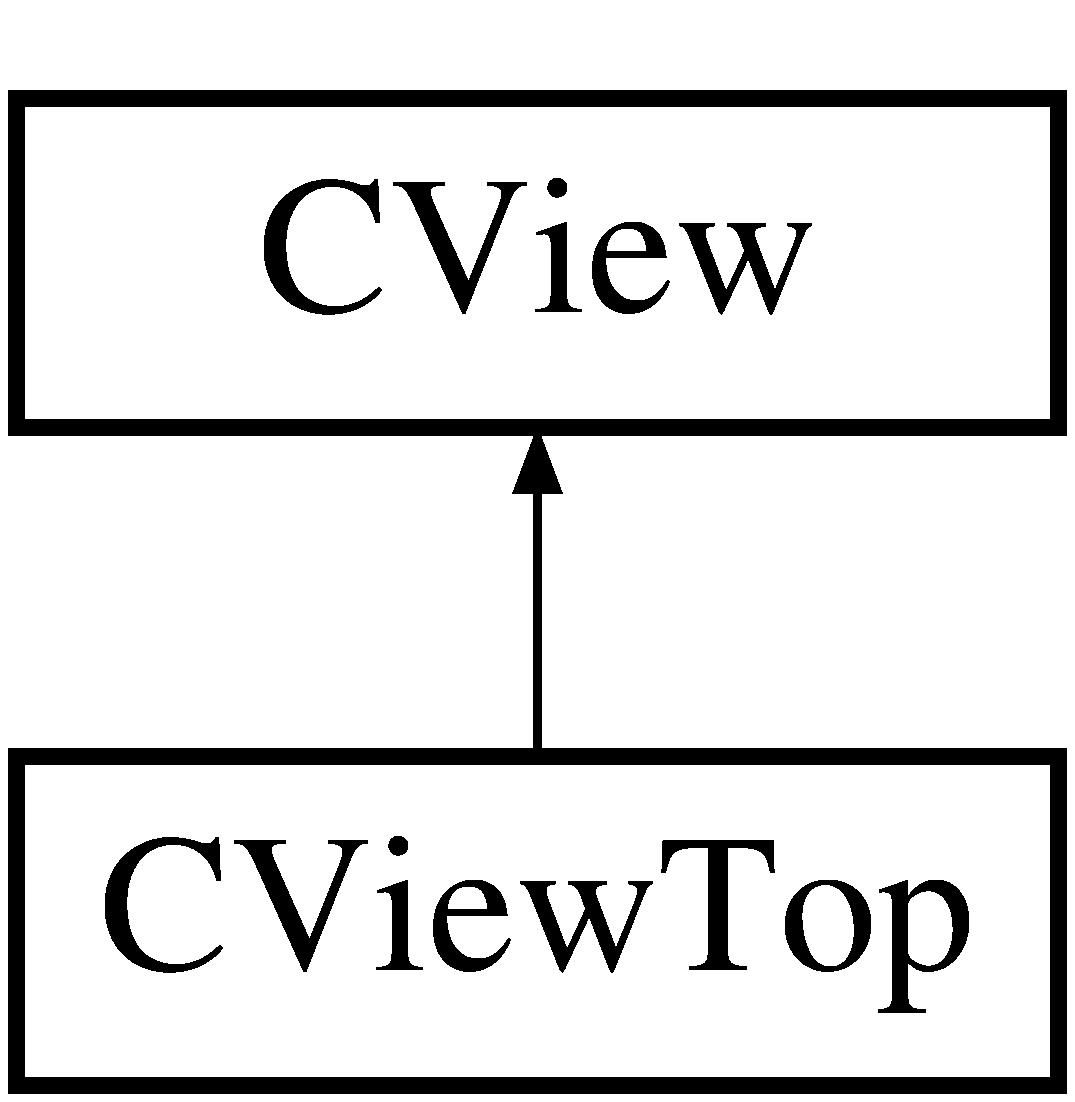
\includegraphics[height=2.000000cm]{class_c_view_top}
\end{center}
\end{figure}
\subsection*{Public Member Functions}
\begin{DoxyCompactItemize}
\item 
virtual void \hyperlink{class_c_view_top_ac4b8af93a75df56478f39feff289f6a6}{On\+Draw} (C\+D\+C $\ast$p\+D\+C)
\item 
\hyperlink{class_c_view_edit}{C\+View\+Edit} $\ast$ \hyperlink{class_c_view_top_a775f50213ecac76ac57016bc402de42a}{Get\+View\+Edit} ()
\item 
\hyperlink{class_c_view_actors}{C\+View\+Actors} $\ast$ \hyperlink{class_c_view_top_a2057cf44f1f7a789b33e2ef8444b6db8}{Get\+View\+Actors} ()
\item 
afx\+\_\+msg int \hyperlink{class_c_view_top_a7e4cad13135855a66719ecb49a8ad3fc}{On\+Create} (L\+P\+C\+R\+E\+A\+T\+E\+S\+T\+R\+U\+C\+T lp\+Create\+Struct)
\item 
afx\+\_\+msg void \hyperlink{class_c_view_top_a171e02fdf1bef80245bbc37d77819f14}{On\+Size} (U\+I\+N\+T n\+Type, int cx, int cy)
\end{DoxyCompactItemize}
\subsection*{Protected Member Functions}
\begin{DoxyCompactItemize}
\item 
\hyperlink{class_c_view_top_a4cee9890cf66890c3cd79efdedf92d1b}{C\+View\+Top} ()
\item 
virtual \hyperlink{class_c_view_top_ad08e0ef0c01e33bb0278dc595467ad8c}{$\sim$\+C\+View\+Top} ()
\end{DoxyCompactItemize}


\subsection{Detailed Description}
Top of the screen view.

This class creates a view that contains a splitter so we can split the top window horizontally. 

\subsection{Constructor \& Destructor Documentation}
\hypertarget{class_c_view_top_a4cee9890cf66890c3cd79efdedf92d1b}{\index{C\+View\+Top@{C\+View\+Top}!C\+View\+Top@{C\+View\+Top}}
\index{C\+View\+Top@{C\+View\+Top}!C\+View\+Top@{C\+View\+Top}}
\subsubsection[{C\+View\+Top}]{\setlength{\rightskip}{0pt plus 5cm}C\+View\+Top\+::\+C\+View\+Top (
\begin{DoxyParamCaption}
{}
\end{DoxyParamCaption}
)\hspace{0.3cm}{\ttfamily [protected]}}}\label{class_c_view_top_a4cee9890cf66890c3cd79efdedf92d1b}
Constructor \hypertarget{class_c_view_top_ad08e0ef0c01e33bb0278dc595467ad8c}{\index{C\+View\+Top@{C\+View\+Top}!````~C\+View\+Top@{$\sim$\+C\+View\+Top}}
\index{````~C\+View\+Top@{$\sim$\+C\+View\+Top}!C\+View\+Top@{C\+View\+Top}}
\subsubsection[{$\sim$\+C\+View\+Top}]{\setlength{\rightskip}{0pt plus 5cm}C\+View\+Top\+::$\sim$\+C\+View\+Top (
\begin{DoxyParamCaption}
{}
\end{DoxyParamCaption}
)\hspace{0.3cm}{\ttfamily [protected]}, {\ttfamily [virtual]}}}\label{class_c_view_top_ad08e0ef0c01e33bb0278dc595467ad8c}
Destructor 

\subsection{Member Function Documentation}
\hypertarget{class_c_view_top_a2057cf44f1f7a789b33e2ef8444b6db8}{\index{C\+View\+Top@{C\+View\+Top}!Get\+View\+Actors@{Get\+View\+Actors}}
\index{Get\+View\+Actors@{Get\+View\+Actors}!C\+View\+Top@{C\+View\+Top}}
\subsubsection[{Get\+View\+Actors}]{\setlength{\rightskip}{0pt plus 5cm}{\bf C\+View\+Actors}$\ast$ C\+View\+Top\+::\+Get\+View\+Actors (
\begin{DoxyParamCaption}
{}
\end{DoxyParamCaption}
)\hspace{0.3cm}{\ttfamily [inline]}}}\label{class_c_view_top_a2057cf44f1f7a789b33e2ef8444b6db8}
Get the View\+Actors window \begin{DoxyReturn}{Returns}
Pointer to View\+Actors window 
\end{DoxyReturn}
\hypertarget{class_c_view_top_a775f50213ecac76ac57016bc402de42a}{\index{C\+View\+Top@{C\+View\+Top}!Get\+View\+Edit@{Get\+View\+Edit}}
\index{Get\+View\+Edit@{Get\+View\+Edit}!C\+View\+Top@{C\+View\+Top}}
\subsubsection[{Get\+View\+Edit}]{\setlength{\rightskip}{0pt plus 5cm}{\bf C\+View\+Edit}$\ast$ C\+View\+Top\+::\+Get\+View\+Edit (
\begin{DoxyParamCaption}
{}
\end{DoxyParamCaption}
)\hspace{0.3cm}{\ttfamily [inline]}}}\label{class_c_view_top_a775f50213ecac76ac57016bc402de42a}
Get the View\+Edit window \begin{DoxyReturn}{Returns}
Pointer to View\+Edit window 
\end{DoxyReturn}
\hypertarget{class_c_view_top_a7e4cad13135855a66719ecb49a8ad3fc}{\index{C\+View\+Top@{C\+View\+Top}!On\+Create@{On\+Create}}
\index{On\+Create@{On\+Create}!C\+View\+Top@{C\+View\+Top}}
\subsubsection[{On\+Create}]{\setlength{\rightskip}{0pt plus 5cm}int C\+View\+Top\+::\+On\+Create (
\begin{DoxyParamCaption}
\item[{L\+P\+C\+R\+E\+A\+T\+E\+S\+T\+R\+U\+C\+T}]{lp\+Create\+Struct}
\end{DoxyParamCaption}
)}}\label{class_c_view_top_a7e4cad13135855a66719ecb49a8ad3fc}
Handle a C\+R\+E\+A\+T\+E message for this window 
\begin{DoxyParams}{Parameters}
{\em lp\+Create\+Struct} & The creation parameter structure \\
\hline
\end{DoxyParams}
\begin{DoxyReturn}{Returns}
0 if successful 
\end{DoxyReturn}
\hypertarget{class_c_view_top_ac4b8af93a75df56478f39feff289f6a6}{\index{C\+View\+Top@{C\+View\+Top}!On\+Draw@{On\+Draw}}
\index{On\+Draw@{On\+Draw}!C\+View\+Top@{C\+View\+Top}}
\subsubsection[{On\+Draw}]{\setlength{\rightskip}{0pt plus 5cm}void C\+View\+Top\+::\+On\+Draw (
\begin{DoxyParamCaption}
\item[{C\+D\+C $\ast$}]{p\+D\+C}
\end{DoxyParamCaption}
)\hspace{0.3cm}{\ttfamily [virtual]}}}\label{class_c_view_top_ac4b8af93a75df56478f39feff289f6a6}
Drawing for this view 
\begin{DoxyParams}{Parameters}
{\em p\+D\+C} & The device context \\
\hline
\end{DoxyParams}
\hypertarget{class_c_view_top_a171e02fdf1bef80245bbc37d77819f14}{\index{C\+View\+Top@{C\+View\+Top}!On\+Size@{On\+Size}}
\index{On\+Size@{On\+Size}!C\+View\+Top@{C\+View\+Top}}
\subsubsection[{On\+Size}]{\setlength{\rightskip}{0pt plus 5cm}void C\+View\+Top\+::\+On\+Size (
\begin{DoxyParamCaption}
\item[{U\+I\+N\+T}]{n\+Type, }
\item[{int}]{cx, }
\item[{int}]{cy}
\end{DoxyParamCaption}
)}}\label{class_c_view_top_a171e02fdf1bef80245bbc37d77819f14}
Handle a new size message 
\begin{DoxyParams}{Parameters}
{\em n\+Type} & Type of size message \\
\hline
{\em cx} & New width \\
\hline
{\em cy} & New height \\
\hline
\end{DoxyParams}


The documentation for this class was generated from the following files\+:\begin{DoxyCompactItemize}
\item 
\hyperlink{_view_top_8h}{View\+Top.\+h}\item 
\hyperlink{_view_top_8cpp}{View\+Top.\+cpp}\end{DoxyCompactItemize}

\chapter{File Documentation}
\hypertarget{_actor_8cpp}{\section{Actor.\+cpp File Reference}
\label{_actor_8cpp}\index{Actor.\+cpp@{Actor.\+cpp}}
}
{\ttfamily \#include \char`\"{}stdafx.\+h\char`\"{}}\\*
{\ttfamily \#include \char`\"{}Actor.\+h\char`\"{}}\\*


\subsection{Detailed Description}
\begin{DoxyAuthor}{Author}
Alexandria Marone 
\end{DoxyAuthor}

\hypertarget{_actor_8h}{\section{Actor.\+h File Reference}
\label{_actor_8h}\index{Actor.\+h@{Actor.\+h}}
}
{\ttfamily \#include $<$string$>$}\\*
{\ttfamily \#include $<$memory$>$}\\*
{\ttfamily \#include $<$vector$>$}\\*
{\ttfamily \#include \char`\"{}Drawable.\+h\char`\"{}}\\*
\subsection*{Classes}
\begin{DoxyCompactItemize}
\item 
class \hyperlink{class_c_actor}{C\+Actor}
\end{DoxyCompactItemize}


\subsection{Detailed Description}
\begin{DoxyAuthor}{Author}
Alexandria Marone
\end{DoxyAuthor}
Class for actors in our drawings 
\hypertarget{_actor_factory_8h}{\section{Actor\+Factory.\+h File Reference}
\label{_actor_factory_8h}\index{Actor\+Factory.\+h@{Actor\+Factory.\+h}}
}
\subsection*{Classes}
\begin{DoxyCompactItemize}
\item 
class \hyperlink{class_c_actor_factory}{C\+Actor\+Factory}
\end{DoxyCompactItemize}


\subsection{Detailed Description}
\begin{DoxyAuthor}{Author}
A marone
\end{DoxyAuthor}
Factory for actors. 
\hypertarget{_canadian_experience_8cpp}{\section{Canadian\+Experience.\+cpp File Reference}
\label{_canadian_experience_8cpp}\index{Canadian\+Experience.\+cpp@{Canadian\+Experience.\+cpp}}
}
{\ttfamily \#include \char`\"{}stdafx.\+h\char`\"{}}\\*
{\ttfamily \#include \char`\"{}afxwinappex.\+h\char`\"{}}\\*
{\ttfamily \#include \char`\"{}afxdialogex.\+h\char`\"{}}\\*
{\ttfamily \#include \char`\"{}Canadian\+Experience.\+h\char`\"{}}\\*
{\ttfamily \#include \char`\"{}Main\+Frm.\+h\char`\"{}}\\*
\subsection*{Classes}
\begin{DoxyCompactItemize}
\item 
class \hyperlink{class_c_about_dlg}{C\+About\+Dlg}
\end{DoxyCompactItemize}
\subsection*{Variables}
\begin{DoxyCompactItemize}
\item 
\hypertarget{_canadian_experience_8cpp_a67124bfb0809a8ff695444fd678f7a94}{\hyperlink{class_c_canadian_experience_app}{C\+Canadian\+Experience\+App} \hyperlink{_canadian_experience_8cpp_a67124bfb0809a8ff695444fd678f7a94}{the\+App}}\label{_canadian_experience_8cpp_a67124bfb0809a8ff695444fd678f7a94}

\begin{DoxyCompactList}\small\item\em The one and only \hyperlink{class_c_canadian_experience_app}{C\+Canadian\+Experience\+App} object. \end{DoxyCompactList}\end{DoxyCompactItemize}


\subsection{Detailed Description}
\begin{DoxyAuthor}{Author}

\end{DoxyAuthor}

\hypertarget{_canadian_experience_8h}{\section{Canadian\+Experience.\+h File Reference}
\label{_canadian_experience_8h}\index{Canadian\+Experience.\+h@{Canadian\+Experience.\+h}}
}
{\ttfamily \#include \char`\"{}resource.\+h\char`\"{}}\\*
\subsection*{Classes}
\begin{DoxyCompactItemize}
\item 
class \hyperlink{class_c_canadian_experience_app}{C\+Canadian\+Experience\+App}
\end{DoxyCompactItemize}
\subsection*{Variables}
\begin{DoxyCompactItemize}
\item 
\hypertarget{_canadian_experience_8h_a67124bfb0809a8ff695444fd678f7a94}{\hyperlink{class_c_canadian_experience_app}{C\+Canadian\+Experience\+App} \hyperlink{_canadian_experience_8h_a67124bfb0809a8ff695444fd678f7a94}{the\+App}}\label{_canadian_experience_8h_a67124bfb0809a8ff695444fd678f7a94}

\begin{DoxyCompactList}\small\item\em The one and only \hyperlink{class_c_canadian_experience_app}{C\+Canadian\+Experience\+App} object. \end{DoxyCompactList}\end{DoxyCompactItemize}


\subsection{Detailed Description}
\begin{DoxyAuthor}{Author}

\end{DoxyAuthor}
Program application class 
\hypertarget{_double_buffer_d_c_8h}{\section{Double\+Buffer\+D\+C.\+h File Reference}
\label{_double_buffer_d_c_8h}\index{Double\+Buffer\+D\+C.\+h@{Double\+Buffer\+D\+C.\+h}}
}


\subsection{Detailed Description}
Customer device context that supports double buffering 
\hypertarget{_drawable_8cpp}{\section{Drawable.\+cpp File Reference}
\label{_drawable_8cpp}\index{Drawable.\+cpp@{Drawable.\+cpp}}
}
{\ttfamily \#include \char`\"{}stdafx.\+h\char`\"{}}\\*
{\ttfamily \#include \char`\"{}Drawable.\+h\char`\"{}}\\*
{\ttfamily \#include $<$cmath$>$}\\*


\subsection{Detailed Description}
\begin{DoxyAuthor}{Author}
A marone 
\end{DoxyAuthor}

\hypertarget{_drawable_8h}{\section{Drawable.\+h File Reference}
\label{_drawable_8h}\index{Drawable.\+h@{Drawable.\+h}}
}
{\ttfamily \#include $<$memory$>$}\\*
{\ttfamily \#include $<$vector$>$}\\*
{\ttfamily \#include $<$string$>$}\\*
\subsection*{Classes}
\begin{DoxyCompactItemize}
\item 
class \hyperlink{class_c_drawable}{C\+Drawable}
\end{DoxyCompactItemize}


\subsection{Detailed Description}
\begin{DoxyAuthor}{Author}
A marone
\end{DoxyAuthor}
Abstract base class for drawable elements of our picture 
\hypertarget{_harold_factory_8h}{\section{Harold\+Factory.\+h File Reference}
\label{_harold_factory_8h}\index{Harold\+Factory.\+h@{Harold\+Factory.\+h}}
}
{\ttfamily \#include $<$memory$>$}\\*
{\ttfamily \#include \char`\"{}Actor.\+h\char`\"{}}\\*
{\ttfamily \#include \char`\"{}Actor\+Factory.\+h\char`\"{}}\\*
\subsection*{Classes}
\begin{DoxyCompactItemize}
\item 
class \hyperlink{class_c_harold_factory}{C\+Harold\+Factory}
\end{DoxyCompactItemize}


\subsection{Detailed Description}
\begin{DoxyAuthor}{Author}
Alexandria Marone
\end{DoxyAuthor}
Class that creates harold char 
\hypertarget{_head_top_8h}{\section{Head\+Top.\+h File Reference}
\label{_head_top_8h}\index{Head\+Top.\+h@{Head\+Top.\+h}}
}
{\ttfamily \#include $<$string$>$}\\*
{\ttfamily \#include \char`\"{}Image\+Drawable.\+h\char`\"{}}\\*
\subsection*{Classes}
\begin{DoxyCompactItemize}
\item 
class \hyperlink{class_c_head_top}{C\+Head\+Top}
\end{DoxyCompactItemize}


\subsection{Detailed Description}
\begin{DoxyAuthor}{Author}
A marone
\end{DoxyAuthor}
Head top class. 
\hypertarget{_image_drawable_8h}{\section{Image\+Drawable.\+h File Reference}
\label{_image_drawable_8h}\index{Image\+Drawable.\+h@{Image\+Drawable.\+h}}
}
{\ttfamily \#include $<$memory$>$}\\*
{\ttfamily \#include \char`\"{}Drawable.\+h\char`\"{}}\\*
\subsection*{Classes}
\begin{DoxyCompactItemize}
\item 
class \hyperlink{class_c_image_drawable}{C\+Image\+Drawable}
\end{DoxyCompactItemize}


\subsection{Detailed Description}
\begin{DoxyAuthor}{Author}
A marone
\end{DoxyAuthor}
Abstract base class for images 
\hypertarget{_main_frm_8cpp}{\section{Main\+Frm.\+cpp File Reference}
\label{_main_frm_8cpp}\index{Main\+Frm.\+cpp@{Main\+Frm.\+cpp}}
}
{\ttfamily \#include \char`\"{}stdafx.\+h\char`\"{}}\\*
{\ttfamily \#include $<$memory$>$}\\*
{\ttfamily \#include \char`\"{}Canadian\+Experience.\+h\char`\"{}}\\*
{\ttfamily \#include \char`\"{}Picture\+Factory.\+h\char`\"{}}\\*
{\ttfamily \#include \char`\"{}Picture.\+h\char`\"{}}\\*
{\ttfamily \#include \char`\"{}Main\+Frm.\+h\char`\"{}}\\*
{\ttfamily \#include \char`\"{}View\+Top.\+h\char`\"{}}\\*


\subsection{Detailed Description}
Implementation of the \hyperlink{class_c_main_frame}{C\+Main\+Frame} class \begin{DoxyAuthor}{Author}
Alexandria Marone 
\end{DoxyAuthor}

\hypertarget{_main_frm_8h}{\section{Main\+Frm.\+h File Reference}
\label{_main_frm_8h}\index{Main\+Frm.\+h@{Main\+Frm.\+h}}
}
{\ttfamily \#include $<$memory$>$}\\*
{\ttfamily \#include \char`\"{}View\+Edit.\+h\char`\"{}}\\*
{\ttfamily \#include \char`\"{}View\+Timeline.\+h\char`\"{}}\\*
{\ttfamily \#include \char`\"{}View\+Actors.\+h\char`\"{}}\\*
\subsection*{Classes}
\begin{DoxyCompactItemize}
\item 
class \hyperlink{class_c_main_frame}{C\+Main\+Frame}
\end{DoxyCompactItemize}


\subsection{Detailed Description}
\begin{DoxyAuthor}{Author}
Alexandria Maarone
\end{DoxyAuthor}
The program main frame. 
\hypertarget{_picture_8cpp}{\section{Picture.\+cpp File Reference}
\label{_picture_8cpp}\index{Picture.\+cpp@{Picture.\+cpp}}
}
{\ttfamily \#include \char`\"{}stdafx.\+h\char`\"{}}\\*
{\ttfamily \#include \char`\"{}Picture.\+h\char`\"{}}\\*
{\ttfamily \#include \char`\"{}Picture\+Observer.\+h\char`\"{}}\\*


\subsection{Detailed Description}
Implementation of the \hyperlink{class_c_main_frame}{C\+Main\+Frame} class \begin{DoxyAuthor}{Author}
Alexandria Marone 
\end{DoxyAuthor}

\hypertarget{_picture_8h}{\section{Picture.\+h File Reference}
\label{_picture_8h}\index{Picture.\+h@{Picture.\+h}}
}
{\ttfamily \#include $<$vector$>$}\\*
{\ttfamily \#include \char`\"{}Actor.\+h\char`\"{}}\\*
\subsection*{Classes}
\begin{DoxyCompactItemize}
\item 
class \hyperlink{class_c_picture}{C\+Picture}
\item 
class \hyperlink{class_c_picture_1_1_actor_iter}{C\+Picture\+::\+Actor\+Iter}
\end{DoxyCompactItemize}


\subsection{Detailed Description}
\begin{DoxyAuthor}{Author}
Alexandria M\+Arone
\end{DoxyAuthor}
Class that provides a view windows for actors. 
\hypertarget{_picture_factory_8cpp}{\section{Picture\+Factory.\+cpp File Reference}
\label{_picture_factory_8cpp}\index{Picture\+Factory.\+cpp@{Picture\+Factory.\+cpp}}
}
{\ttfamily \#include \char`\"{}stdafx.\+h\char`\"{}}\\*
{\ttfamily \#include $<$memory$>$}\\*
{\ttfamily \#include \char`\"{}Picture\+Factory.\+h\char`\"{}}\\*
{\ttfamily \#include \char`\"{}Harold\+Factory.\+h\char`\"{}}\\*
{\ttfamily \#include \char`\"{}Picture.\+h\char`\"{}}\\*
{\ttfamily \#include \char`\"{}Image\+Drawable.\+h\char`\"{}}\\*
{\ttfamily \#include \char`\"{}Quinn\+Factory.\+h\char`\"{}}\\*


\subsection{Detailed Description}
\begin{DoxyAuthor}{Author}
Alexandria Marone 
\end{DoxyAuthor}

\hypertarget{_picture_observer_8cpp}{\section{Picture\+Observer.\+cpp File Reference}
\label{_picture_observer_8cpp}\index{Picture\+Observer.\+cpp@{Picture\+Observer.\+cpp}}
}
{\ttfamily \#include \char`\"{}stdafx.\+h\char`\"{}}\\*
{\ttfamily \#include \char`\"{}Picture\+Observer.\+h\char`\"{}}\\*
{\ttfamily \#include \char`\"{}Picture.\+h\char`\"{}}\\*


\subsection{Detailed Description}
\begin{DoxyAuthor}{Author}
Alexandria Marone
\end{DoxyAuthor}
Class that provides a view windows for actors. 
\hypertarget{_picture_observer_8h}{\section{Picture\+Observer.\+h File Reference}
\label{_picture_observer_8h}\index{Picture\+Observer.\+h@{Picture\+Observer.\+h}}
}
{\ttfamily \#include $<$memory$>$}\\*
{\ttfamily \#include \char`\"{}Picture.\+h\char`\"{}}\\*
\subsection*{Classes}
\begin{DoxyCompactItemize}
\item 
class \hyperlink{class_c_picture_observer}{C\+Picture\+Observer}
\end{DoxyCompactItemize}


\subsection{Detailed Description}
\begin{DoxyAuthor}{Author}
Alexandria Marone
\end{DoxyAuthor}
Class that provides a view windows for actors. 
\hypertarget{_poly_drawable_8h}{\section{Poly\+Drawable.\+h File Reference}
\label{_poly_drawable_8h}\index{Poly\+Drawable.\+h@{Poly\+Drawable.\+h}}
}
{\ttfamily \#include $<$vector$>$}\\*
{\ttfamily \#include \char`\"{}Drawable.\+h\char`\"{}}\\*
\subsection*{Classes}
\begin{DoxyCompactItemize}
\item 
class \hyperlink{class_c_poly_drawable}{C\+Poly\+Drawable}
\end{DoxyCompactItemize}


\subsection{Detailed Description}
\begin{DoxyAuthor}{Author}
A marone
\end{DoxyAuthor}
Abstract base class for drawable elements of our picture 
\hypertarget{_quinn_factory_8cpp}{\section{Quinn\+Factory.\+cpp File Reference}
\label{_quinn_factory_8cpp}\index{Quinn\+Factory.\+cpp@{Quinn\+Factory.\+cpp}}
}
{\ttfamily \#include \char`\"{}stdafx.\+h\char`\"{}}\\*
{\ttfamily \#include $<$memory$>$}\\*
{\ttfamily \#include \char`\"{}Actor.\+h\char`\"{}}\\*
{\ttfamily \#include \char`\"{}Poly\+Drawable.\+h\char`\"{}}\\*
{\ttfamily \#include \char`\"{}Quinn\+Factory.\+h\char`\"{}}\\*
{\ttfamily \#include \char`\"{}Image\+Drawable.\+h\char`\"{}}\\*
{\ttfamily \#include \char`\"{}Head\+Top.\+h\char`\"{}}\\*


\subsection{Detailed Description}
\begin{DoxyAuthor}{Author}
Alexandria Marone 
\end{DoxyAuthor}

\hypertarget{_quinn_factory_8h}{\section{Quinn\+Factory.\+h File Reference}
\label{_quinn_factory_8h}\index{Quinn\+Factory.\+h@{Quinn\+Factory.\+h}}
}
{\ttfamily \#include $<$memory$>$}\\*
{\ttfamily \#include \char`\"{}Actor.\+h\char`\"{}}\\*
{\ttfamily \#include \char`\"{}Actor\+Factory.\+h\char`\"{}}\\*
\subsection*{Classes}
\begin{DoxyCompactItemize}
\item 
class \hyperlink{class_c_quinn_factory}{C\+Quinn\+Factory}
\end{DoxyCompactItemize}


\subsection{Detailed Description}
\begin{DoxyAuthor}{Author}
Alexandria Marone
\end{DoxyAuthor}
Class that creates Quinn char 
\hypertarget{_view_actors_8cpp}{\section{View\+Actors.\+cpp File Reference}
\label{_view_actors_8cpp}\index{View\+Actors.\+cpp@{View\+Actors.\+cpp}}
}
{\ttfamily \#include \char`\"{}stdafx.\+h\char`\"{}}\\*
{\ttfamily \#include \char`\"{}Canadian\+Experience.\+h\char`\"{}}\\*
{\ttfamily \#include \char`\"{}View\+Actors.\+h\char`\"{}}\\*
{\ttfamily \#include \char`\"{}Double\+Buffer\+D\+C.\+h\char`\"{}}\\*


\subsection{Detailed Description}
\begin{DoxyAuthor}{Author}

\end{DoxyAuthor}

\hypertarget{_view_actors_8h}{\section{View\+Actors.\+h File Reference}
\label{_view_actors_8h}\index{View\+Actors.\+h@{View\+Actors.\+h}}
}
{\ttfamily \#include \char`\"{}Picture\+Observer.\+h\char`\"{}}\\*
\subsection*{Classes}
\begin{DoxyCompactItemize}
\item 
class \hyperlink{class_c_view_actors}{C\+View\+Actors}
\end{DoxyCompactItemize}


\subsection{Detailed Description}
\begin{DoxyAuthor}{Author}
Alexandria Marone
\end{DoxyAuthor}
Class that provides a view windows for actors. 
\hypertarget{_view_edit_8cpp}{\section{View\+Edit.\+cpp File Reference}
\label{_view_edit_8cpp}\index{View\+Edit.\+cpp@{View\+Edit.\+cpp}}
}
{\ttfamily \#include \char`\"{}stdafx.\+h\char`\"{}}\\*
{\ttfamily \#include \char`\"{}Picture.\+h\char`\"{}}\\*
{\ttfamily \#include \char`\"{}Canadian\+Experience.\+h\char`\"{}}\\*
{\ttfamily \#include \char`\"{}View\+Edit.\+h\char`\"{}}\\*
{\ttfamily \#include \char`\"{}Double\+Buffer\+D\+C.\+h\char`\"{}}\\*
{\ttfamily \#include \char`\"{}Main\+Frm.\+h\char`\"{}}\\*
\subsection*{Variables}
\begin{DoxyCompactItemize}
\item 
\hypertarget{_view_edit_8cpp_a5aad50df163545659b29dc0f88c8a2d4}{const double \hyperlink{_view_edit_8cpp_a5aad50df163545659b29dc0f88c8a2d4}{Rotation\+Scaling} = 0.\+02}\label{_view_edit_8cpp_a5aad50df163545659b29dc0f88c8a2d4}

\begin{DoxyCompactList}\small\item\em A scaling factor, converts mouse motion to rotation in radians. \end{DoxyCompactList}\end{DoxyCompactItemize}


\subsection{Detailed Description}
\begin{DoxyAuthor}{Author}
Alexandria Marone 
\end{DoxyAuthor}

\hypertarget{_view_edit_8h}{\section{View\+Edit.\+h File Reference}
\label{_view_edit_8h}\index{View\+Edit.\+h@{View\+Edit.\+h}}
}
{\ttfamily \#include \char`\"{}Picture\+Observer.\+h\char`\"{}}\\*
\subsection*{Classes}
\begin{DoxyCompactItemize}
\item 
class \hyperlink{class_c_view_edit}{C\+View\+Edit}
\end{DoxyCompactItemize}


\subsection{Detailed Description}
\begin{DoxyAuthor}{Author}
Alexandria Marone
\end{DoxyAuthor}
View class the provides a window for editing our pixture 
\hypertarget{_view_timeline_8cpp}{\section{View\+Timeline.\+cpp File Reference}
\label{_view_timeline_8cpp}\index{View\+Timeline.\+cpp@{View\+Timeline.\+cpp}}
}
{\ttfamily \#include \char`\"{}stdafx.\+h\char`\"{}}\\*
{\ttfamily \#include \char`\"{}Canadian\+Experience.\+h\char`\"{}}\\*
{\ttfamily \#include \char`\"{}View\+Timeline.\+h\char`\"{}}\\*
{\ttfamily \#include \char`\"{}Double\+Buffer\+D\+C.\+h\char`\"{}}\\*
{\ttfamily \#include \char`\"{}Main\+Frm.\+h\char`\"{}}\\*


\subsection{Detailed Description}
\begin{DoxyAuthor}{Author}

\end{DoxyAuthor}

\hypertarget{_view_timeline_8h}{\section{View\+Timeline.\+h File Reference}
\label{_view_timeline_8h}\index{View\+Timeline.\+h@{View\+Timeline.\+h}}
}
{\ttfamily \#include \char`\"{}Picture\+Observer.\+h\char`\"{}}\\*
\subsection*{Classes}
\begin{DoxyCompactItemize}
\item 
class \hyperlink{class_c_view_timeline}{C\+View\+Timeline}
\end{DoxyCompactItemize}


\subsection{Detailed Description}
\begin{DoxyAuthor}{Author}
Alexandria Marone
\end{DoxyAuthor}
View window for the animation timeline 
\hypertarget{_view_top_8cpp}{\section{View\+Top.\+cpp File Reference}
\label{_view_top_8cpp}\index{View\+Top.\+cpp@{View\+Top.\+cpp}}
}
{\ttfamily \#include \char`\"{}stdafx.\+h\char`\"{}}\\*
{\ttfamily \#include \char`\"{}Canadian\+Experience.\+h\char`\"{}}\\*
{\ttfamily \#include \char`\"{}View\+Top.\+h\char`\"{}}\\*
{\ttfamily \#include \char`\"{}View\+Actors.\+h\char`\"{}}\\*
{\ttfamily \#include \char`\"{}View\+Edit.\+h\char`\"{}}\\*
{\ttfamily \#include \char`\"{}View\+Timeline.\+h\char`\"{}}\\*


\subsection{Detailed Description}
\begin{DoxyAuthor}{Author}
Charles B. Owen 
\end{DoxyAuthor}

\hypertarget{_view_top_8h}{\section{View\+Top.\+h File Reference}
\label{_view_top_8h}\index{View\+Top.\+h@{View\+Top.\+h}}
}
{\ttfamily \#include \char`\"{}View\+Edit.\+h\char`\"{}}\\*
{\ttfamily \#include \char`\"{}View\+Actors.\+h\char`\"{}}\\*
\subsection*{Classes}
\begin{DoxyCompactItemize}
\item 
class \hyperlink{class_c_view_top}{C\+View\+Top}
\end{DoxyCompactItemize}


\subsection{Detailed Description}
\begin{DoxyAuthor}{Author}
Charles B. Owen
\end{DoxyAuthor}
Class for the top of the screen view.

You should not have to change this file. 
%--- End generated contents ---

% Index
\newpage
\phantomsection
\addcontentsline{toc}{chapter}{Index}
\printindex

\end{document}
